\documentclass{book}
\usepackage[a4paper,top=2.5cm,bottom=2.5cm,left=2.5cm,right=2.5cm]{geometry}
\usepackage{makeidx}
\usepackage{natbib}
\usepackage{graphicx}
\usepackage{multicol}
\usepackage{float}
\usepackage{listings}
\usepackage{color}
\usepackage{ifthen}
\usepackage[table]{xcolor}
\usepackage{textcomp}
\usepackage{alltt}
\usepackage{ifpdf}
\ifpdf
\usepackage[pdftex,
            pagebackref=true,
            colorlinks=true,
            linkcolor=blue,
            unicode
           ]{hyperref}
\else
\usepackage[ps2pdf,
            pagebackref=true,
            colorlinks=true,
            linkcolor=blue,
            unicode
           ]{hyperref}
\usepackage{pspicture}
\fi
\usepackage[utf8]{inputenc}
\usepackage{mathptmx}
\usepackage[scaled=.90]{helvet}
\usepackage{courier}
\usepackage{sectsty}
\usepackage[titles]{tocloft}
\usepackage{doxygen}
\lstset{language=C++,inputencoding=utf8,basicstyle=\footnotesize,breaklines=true,breakatwhitespace=true,tabsize=4,numbers=left }
\makeindex
\setcounter{tocdepth}{3}
\renewcommand{\footrulewidth}{0.4pt}
\renewcommand{\familydefault}{\sfdefault}
\hfuzz=15pt
\setlength{\emergencystretch}{15pt}
\hbadness=750
\tolerance=750
\begin{document}
\hypersetup{pageanchor=false,citecolor=blue}
\begin{titlepage}
\vspace*{7cm}
\begin{center}
{\Large S\-Y\-M\-M\-E\-T\-R\-Y }\\
\vspace*{1cm}
{\large Generated by Doxygen 1.8.1.1}\\
\vspace*{0.5cm}
{\small Mon Dec 24 2012 14:51:04}\\
\end{center}
\end{titlepage}
\clearemptydoublepage
\pagenumbering{roman}
\tableofcontents
\clearemptydoublepage
\pagenumbering{arabic}
\hypersetup{pageanchor=true,citecolor=blue}
\chapter{S\-Y\-M\-M\-E\-T\-R\-Y}
\label{index}\hypertarget{index}{}\begin{DoxyAuthor}{Author}
A\-N\-D\-R\-E\-I M\-I\-L\-E\-A
\end{DoxyAuthor}
Computational library(numerical recipes, symbolic computation, etc). 
\chapter{Class Index}
\section{Class Hierarchy}
This inheritance list is sorted roughly, but not completely, alphabetically\-:\begin{DoxyCompactList}
\item \contentsline{section}{Addition}{\pageref{classAddition}}{}
\item \contentsline{section}{tree\-:\-:btree\-\_\-iterator$<$ T, N $>$}{\pageref{classtree_1_1btree__iterator}}{}
\begin{DoxyCompactList}
\item \contentsline{section}{tree\-:\-:btree\-\_\-inorder\-\_\-iterator$<$ T, N $>$}{\pageref{classtree_1_1btree__inorder__iterator}}{}
\item \contentsline{section}{tree\-:\-:btree\-\_\-postorder\-\_\-iterator$<$ T, N $>$}{\pageref{classtree_1_1btree__postorder__iterator}}{}
\item \contentsline{section}{tree\-:\-:btree\-\_\-preorder\-\_\-iterator$<$ T, N $>$}{\pageref{classtree_1_1btree__preorder__iterator}}{}
\end{DoxyCompactList}
\item \contentsline{section}{tree\-:\-:btree\-\_\-iterator$<$ T, btree\-\_\-threaded\-\_\-node$<$ T $>$ $>$}{\pageref{classtree_1_1btree__iterator_3_01T_00_01btree__threaded__node_3_01T_01_4_01_4}}{}
\begin{DoxyCompactList}
\item \contentsline{section}{tree\-:\-:btree\-\_\-inorder\-\_\-iterator$<$ T, btree\-\_\-threaded\-\_\-node$<$ T $>$ $>$}{\pageref{classtree_1_1btree__inorder__iterator_3_01T_00_01btree__threaded__node_3_01T_01_4_01_4}}{}
\end{DoxyCompactList}
\item \contentsline{section}{tree\-:\-:btree\-\_\-node$<$ T $>$}{\pageref{structtree_1_1btree__node}}{}
\item \contentsline{section}{tree\-:\-:btree\-\_\-threaded\-\_\-node$<$ T $>$}{\pageref{structtree_1_1btree__threaded__node}}{}
\item \contentsline{section}{tree\-:\-:c\-Binary\-Rep$<$ T $>$}{\pageref{classtree_1_1cBinaryRep}}{}
\item \contentsline{section}{tree\-:\-:c\-Binary\-Tree$<$ T, R\-E\-P $>$}{\pageref{classtree_1_1cBinaryTree}}{}
\item \contentsline{section}{c\-Cayley\-Grf$<$ G $>$}{\pageref{classcCayleyGrf}}{}
\item \contentsline{section}{c\-Cayley\-Grf$<$ G $>$\-:\-:c\-Colour\-Edges\-Vis$<$ E, Grf $>$}{\pageref{classcCayleyGrf_1_1cColourEdgesVis}}{}
\item \contentsline{section}{c\-Gen\-Rep$<$ T $>$}{\pageref{classcGenRep}}{}
\item \contentsline{section}{c\-Group$<$ T, group\-\_\-rep $>$}{\pageref{classcGroup}}{}
\item \contentsline{section}{c\-Group\-Elem$<$ T, Binary\-Op $>$}{\pageref{classcGroupElem}}{}
\item \contentsline{section}{c\-Group\-Relation}{\pageref{classcGroupRelation}}{}
\item \contentsline{section}{c\-Grp\-Lattice$<$ G $>$}{\pageref{classcGrpLattice}}{}
\item \contentsline{section}{c\-Homomorphism$<$ G1, G2 $>$}{\pageref{classcHomomorphism}}{}
\item \contentsline{section}{c\-Int\-Mod\-N\-Elem$<$ N $>$}{\pageref{classcIntModNElem}}{}
\item \contentsline{section}{Composition}{\pageref{classComposition}}{}
\item \contentsline{section}{c\-Perm\-Elem}{\pageref{classcPermElem}}{}
\item \contentsline{section}{c\-S\-L\-P\-Rep$<$ T $>$}{\pageref{classcSLPRep}}{}
\item \contentsline{section}{c\-Subgroup$<$ G $>$}{\pageref{classcSubgroup}}{}
\item \contentsline{section}{c\-Symmetric\-Rep$<$ T $>$}{\pageref{classcSymmetricRep}}{}
\item \contentsline{section}{tree\-:\-:c\-Threaded\-Rep$<$ T $>$}{\pageref{classtree_1_1cThreadedRep}}{}
\item \contentsline{section}{Factorial$<$ V\-A\-L $>$}{\pageref{structFactorial}}{}
\item \contentsline{section}{Factorial$<$ 0 $>$}{\pageref{structFactorial_3_010_01_4}}{}
\item \contentsline{section}{Multiplication}{\pageref{classMultiplication}}{}
\end{DoxyCompactList}

\chapter{Class Index}
\section{\-Class \-List}
\-Here are the classes, structs, unions and interfaces with brief descriptions\-:\begin{DoxyCompactList}
\item\contentsline{section}{\hyperlink{classengine_1_1cGroupGenCommand_1_1AddGrpGen}{engine\-::c\-Group\-Gen\-Command\-::\-Add\-Grp\-Gen} }{\pageref{classengine_1_1cGroupGenCommand_1_1AddGrpGen}}{}
\item\contentsline{section}{\hyperlink{classengine_1_1cCommand}{engine\-::c\-Command} }{\pageref{classengine_1_1cCommand}}{}
\item\contentsline{section}{\hyperlink{classengine_1_1cCommandCreator}{engine\-::c\-Command\-Creator$<$ C\-R\-E\-A\-T\-O\-R $>$} }{\pageref{classengine_1_1cCommandCreator}}{}
\item\contentsline{section}{\hyperlink{classengine_1_1cCommandQueue}{engine\-::c\-Command\-Queue} }{\pageref{classengine_1_1cCommandQueue}}{}
\item\contentsline{section}{\hyperlink{classengine_1_1cCreator}{engine\-::c\-Creator} }{\pageref{classengine_1_1cCreator}}{}
\item\contentsline{section}{\hyperlink{classengine_1_1cEstimator}{engine\-::c\-Estimator} }{\pageref{classengine_1_1cEstimator}}{}
\item\contentsline{section}{\hyperlink{classengine_1_1cGetElemCommand}{engine\-::c\-Get\-Elem\-Command} }{\pageref{classengine_1_1cGetElemCommand}}{}
\item\contentsline{section}{\hyperlink{classengine_1_1cGetSubgrpCommand}{engine\-::c\-Get\-Subgrp\-Command} }{\pageref{classengine_1_1cGetSubgrpCommand}}{}
\item\contentsline{section}{\hyperlink{classcGroupFactory}{c\-Group\-Factory} }{\pageref{classcGroupFactory}}{}
\item\contentsline{section}{\hyperlink{classengine_1_1cGroupGenCommand}{engine\-::c\-Group\-Gen\-Command} }{\pageref{classengine_1_1cGroupGenCommand}}{}
\item\contentsline{section}{\hyperlink{classcInterpreter}{c\-Interpreter} }{\pageref{classcInterpreter}}{}
\item\contentsline{section}{\hyperlink{classengine_1_1cLogger}{engine\-::c\-Logger} }{\pageref{classengine_1_1cLogger}}{}
\item\contentsline{section}{\hyperlink{classengine_1_1cResult}{engine\-::c\-Result} }{\pageref{classengine_1_1cResult}}{}
\item\contentsline{section}{\hyperlink{classcSerializer_3_01SymmGrpElem_00_01CONT_01_4}{c\-Serializer$<$ Symm\-Grp\-Elem, C\-O\-N\-T $>$} }{\pageref{classcSerializer_3_01SymmGrpElem_00_01CONT_01_4}}{}
\item\contentsline{section}{\hyperlink{classengine_1_1cSession}{engine\-::c\-Session} }{\pageref{classengine_1_1cSession}}{}
\item\contentsline{section}{\hyperlink{classengine_1_1cThreadPool}{engine\-::c\-Thread\-Pool} }{\pageref{classengine_1_1cThreadPool}}{}
\item\contentsline{section}{\hyperlink{classengine_1_1cVariantVisitor}{engine\-::c\-Variant\-Visitor} }{\pageref{classengine_1_1cVariantVisitor}}{}
\item\contentsline{section}{\hyperlink{structengine_1_1cGroupGenCommand_1_1group__type__}{engine\-::c\-Group\-Gen\-Command\-::group\-\_\-type\-\_\-} }{\pageref{structengine_1_1cGroupGenCommand_1_1group__type__}}{}
\end{DoxyCompactList}

\chapter{Class Documentation}
\hypertarget{classAddition}{\section{Addition Class Reference}
\label{classAddition}\index{Addition@{Addition}}
}


{\ttfamily \#include $<$binary\-\_\-op.\-h$>$}



Collaboration diagram for Addition\-:
\subsection*{Public Member Functions}
\begin{DoxyCompactItemize}
\item 
\hypertarget{classAddition_a0cd0e60cd506c9e640d89422303d77b7}{{\footnotesize template$<$typename T $>$ }\\T {\bfseries operator()} (const T \&ob1, const T \&ob2) const }\label{classAddition_a0cd0e60cd506c9e640d89422303d77b7}

\end{DoxyCompactItemize}
\subsection*{Static Public Attributes}
\begin{DoxyCompactItemize}
\item 
\hypertarget{classAddition_a24b52cf787fbb2997cca7fabd26feb9b}{static const bool {\bfseries is\-Additive} = true}\label{classAddition_a24b52cf787fbb2997cca7fabd26feb9b}

\item 
\hypertarget{classAddition_a5e060aac1855b53aa87849ea9e439cd9}{static const bool {\bfseries is\-Multiplicative} = false}\label{classAddition_a5e060aac1855b53aa87849ea9e439cd9}

\item 
\hypertarget{classAddition_a7fce2d48cdd7335298e138775b9fde7b}{static const bool {\bfseries is\-Composition} = false}\label{classAddition_a7fce2d48cdd7335298e138775b9fde7b}

\end{DoxyCompactItemize}


\subsection{Detailed Description}
class that represents the addition binary operation used also as a template policy 

The documentation for this class was generated from the following file\-:\begin{DoxyCompactItemize}
\item 
binary\-\_\-op.\-h\end{DoxyCompactItemize}

\hypertarget{classtree_1_1btree__inorder__iterator}{\section{tree\-:\-:btree\-\_\-inorder\-\_\-iterator$<$ T, N $>$ Class Template Reference}
\label{classtree_1_1btree__inorder__iterator}\index{tree\-::btree\-\_\-inorder\-\_\-iterator$<$ T, N $>$@{tree\-::btree\-\_\-inorder\-\_\-iterator$<$ T, N $>$}}
}


{\ttfamily \#include $<$binary\-\_\-tree\-\_\-iter.\-h$>$}



Inheritance diagram for tree\-:\-:btree\-\_\-inorder\-\_\-iterator$<$ T, N $>$\-:
\nopagebreak
\begin{figure}[H]
\begin{center}
\leavevmode
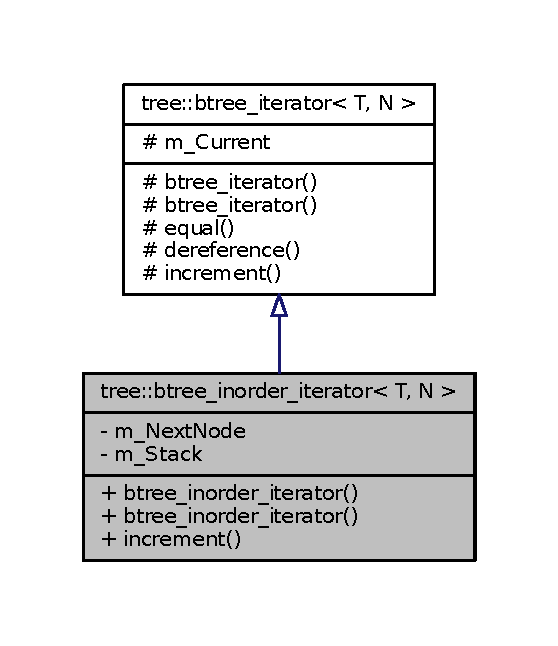
\includegraphics[width=264pt]{classtree_1_1btree__inorder__iterator__inherit__graph}
\end{center}
\end{figure}


Collaboration diagram for tree\-:\-:btree\-\_\-inorder\-\_\-iterator$<$ T, N $>$\-:
\nopagebreak
\begin{figure}[H]
\begin{center}
\leavevmode
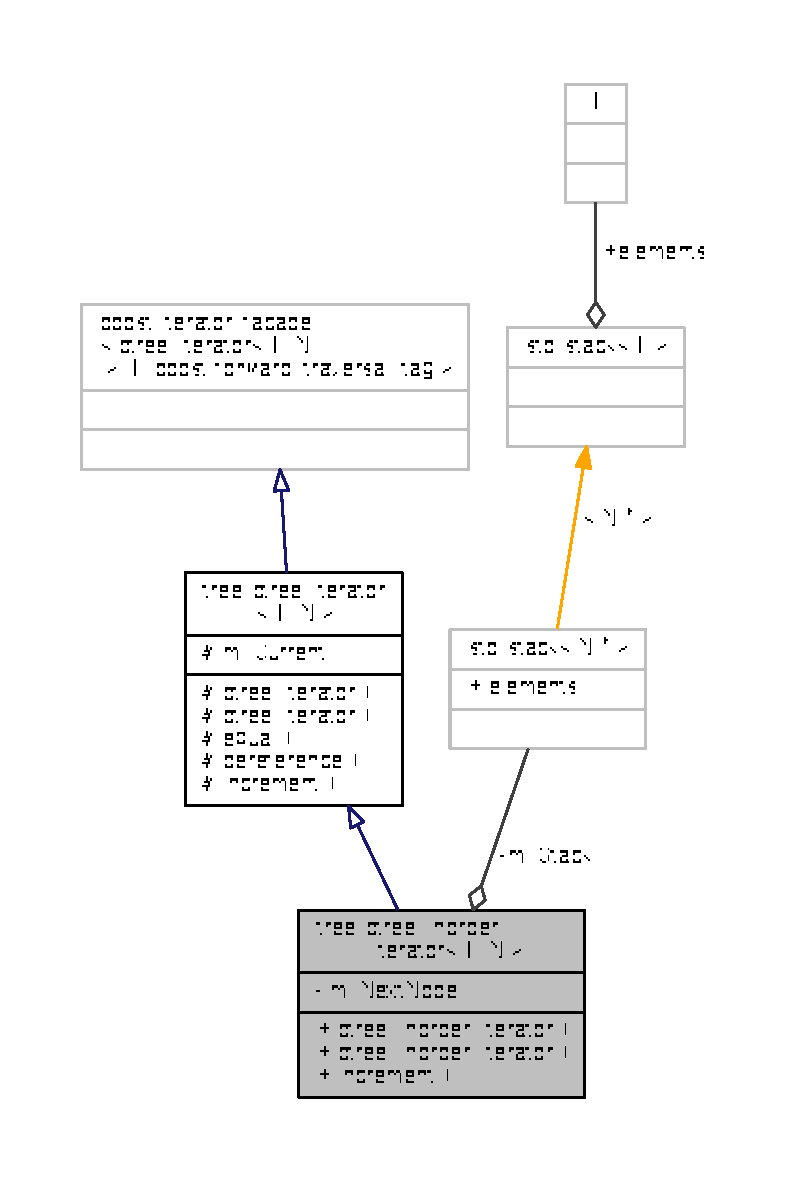
\includegraphics[width=350pt]{classtree_1_1btree__inorder__iterator__coll__graph}
\end{center}
\end{figure}
\subsection*{Public Member Functions}
\begin{DoxyCompactItemize}
\item 
\hypertarget{classtree_1_1btree__inorder__iterator_abb3121aadd921041e0af5a28d527eaf2}{{\bfseries btree\-\_\-inorder\-\_\-iterator} (N $\ast$node)}\label{classtree_1_1btree__inorder__iterator_abb3121aadd921041e0af5a28d527eaf2}

\item 
\hypertarget{classtree_1_1btree__inorder__iterator_ae42f42822641ec3d55e2e570f9e0d897}{void {\bfseries increment} ()}\label{classtree_1_1btree__inorder__iterator_ae42f42822641ec3d55e2e570f9e0d897}

\end{DoxyCompactItemize}
\subsection*{Private Attributes}
\begin{DoxyCompactItemize}
\item 
\hypertarget{classtree_1_1btree__inorder__iterator_aa2586ca852a9b462b0774af427a7a10f}{N $\ast$ {\bfseries m\-\_\-\-Next\-Node}}\label{classtree_1_1btree__inorder__iterator_aa2586ca852a9b462b0774af427a7a10f}

\item 
\hypertarget{classtree_1_1btree__inorder__iterator_a35c2412b7ad6f89a8ca7eeb2eef3f413}{std\-::stack$<$ N $\ast$ $>$ {\bfseries m\-\_\-\-Stack}}\label{classtree_1_1btree__inorder__iterator_a35c2412b7ad6f89a8ca7eeb2eef3f413}

\end{DoxyCompactItemize}
\subsection*{Additional Inherited Members}


\subsection{Detailed Description}
\subsubsection*{template$<$typename T, typename N$>$class tree\-::btree\-\_\-inorder\-\_\-iterator$<$ T, N $>$}

traverses the tree in inorder(symmetric order -- left, root, right) using a stack 

The documentation for this class was generated from the following file\-:\begin{DoxyCompactItemize}
\item 
tree/binary\-\_\-tree\-\_\-iter.\-h\end{DoxyCompactItemize}

\hypertarget{classtree_1_1btree__inorder__iterator_3_01T_00_01btree__threaded__node_3_01T_01_4_01_4}{\section{tree\-:\-:btree\-\_\-inorder\-\_\-iterator$<$ T, btree\-\_\-threaded\-\_\-node$<$ T $>$ $>$ Class Template Reference}
\label{classtree_1_1btree__inorder__iterator_3_01T_00_01btree__threaded__node_3_01T_01_4_01_4}\index{tree\-::btree\-\_\-inorder\-\_\-iterator$<$ T, btree\-\_\-threaded\-\_\-node$<$ T $>$ $>$@{tree\-::btree\-\_\-inorder\-\_\-iterator$<$ T, btree\-\_\-threaded\-\_\-node$<$ T $>$ $>$}}
}


{\ttfamily \#include $<$binary\-\_\-tree\-\_\-iter.\-h$>$}



Inheritance diagram for tree\-:\-:btree\-\_\-inorder\-\_\-iterator$<$ T, btree\-\_\-threaded\-\_\-node$<$ T $>$ $>$\-:
\nopagebreak
\begin{figure}[H]
\begin{center}
\leavevmode
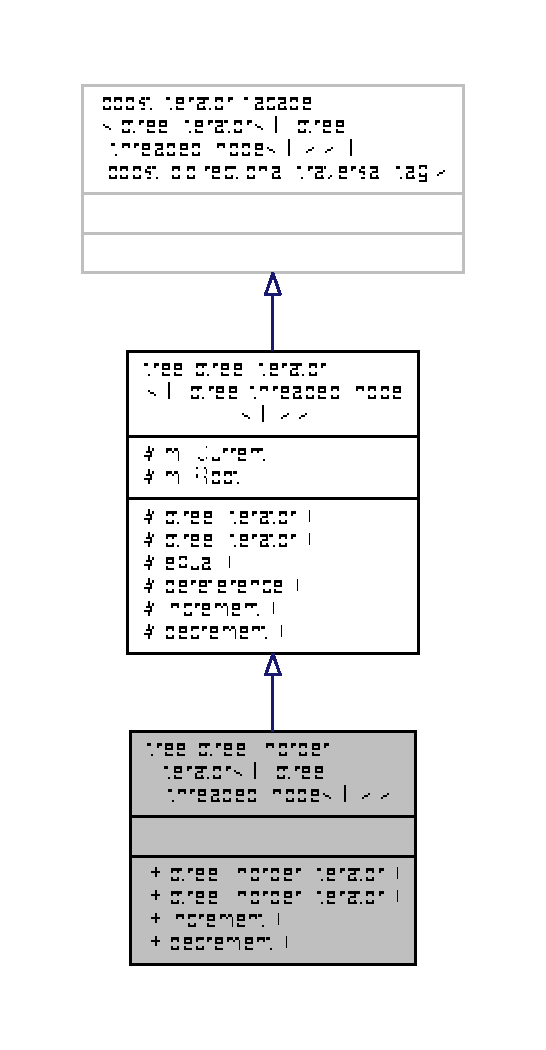
\includegraphics[width=262pt]{classtree_1_1btree__inorder__iterator_3_01T_00_01btree__threaded__node_3_01T_01_4_01_4__inherit__graph}
\end{center}
\end{figure}


Collaboration diagram for tree\-:\-:btree\-\_\-inorder\-\_\-iterator$<$ T, btree\-\_\-threaded\-\_\-node$<$ T $>$ $>$\-:
\nopagebreak
\begin{figure}[H]
\begin{center}
\leavevmode
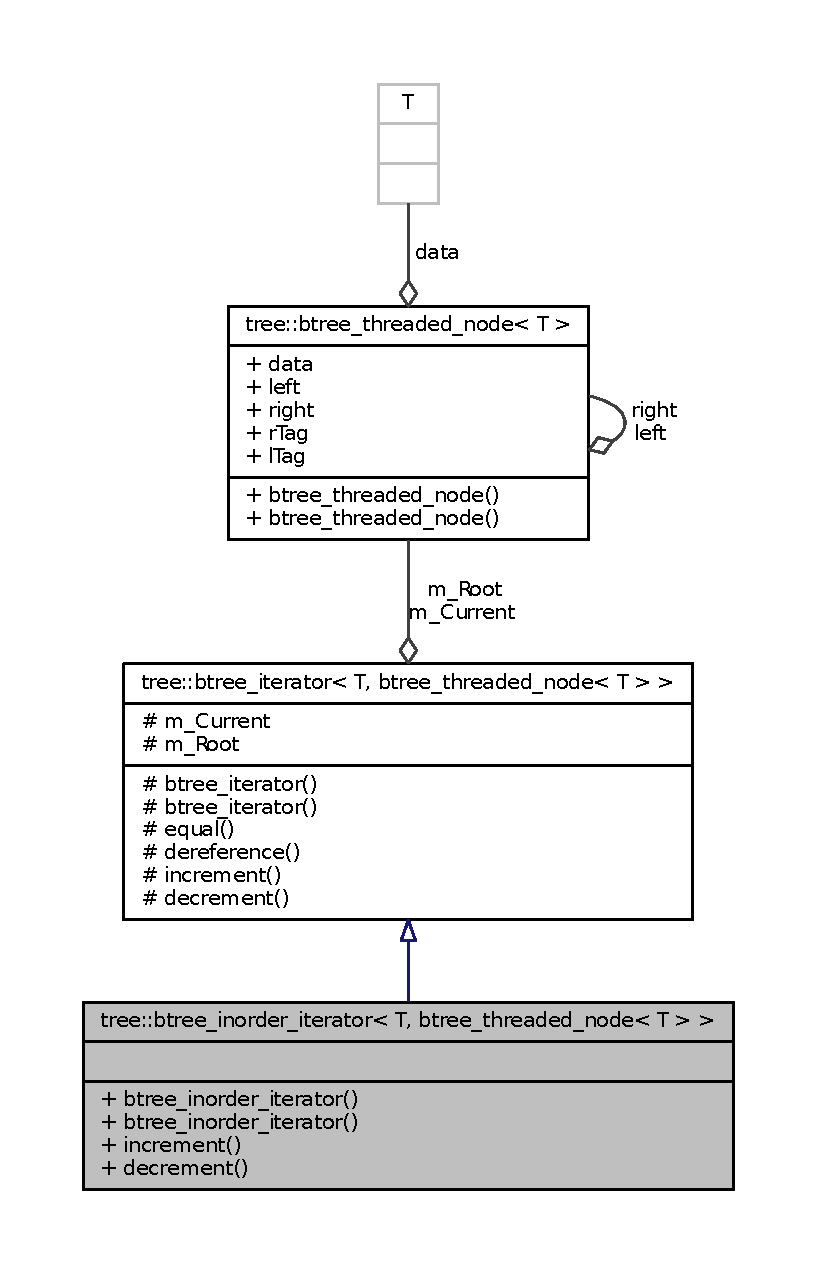
\includegraphics[width=350pt]{classtree_1_1btree__inorder__iterator_3_01T_00_01btree__threaded__node_3_01T_01_4_01_4__coll__graph}
\end{center}
\end{figure}
\subsection*{Public Member Functions}
\begin{DoxyCompactItemize}
\item 
\hypertarget{classtree_1_1btree__inorder__iterator_3_01T_00_01btree__threaded__node_3_01T_01_4_01_4_afd6683f0b4f5a8336d41497ed5d442d9}{{\bfseries btree\-\_\-inorder\-\_\-iterator} (\hyperlink{structtree_1_1btree__threaded__node}{N} $\ast$node, \hyperlink{structtree_1_1btree__threaded__node}{N} $\ast$root)}\label{classtree_1_1btree__inorder__iterator_3_01T_00_01btree__threaded__node_3_01T_01_4_01_4_afd6683f0b4f5a8336d41497ed5d442d9}

\item 
\hypertarget{classtree_1_1btree__inorder__iterator_3_01T_00_01btree__threaded__node_3_01T_01_4_01_4_ad7bab9e59be6a764fd33a2aa7b938217}{void {\bfseries increment} ()}\label{classtree_1_1btree__inorder__iterator_3_01T_00_01btree__threaded__node_3_01T_01_4_01_4_ad7bab9e59be6a764fd33a2aa7b938217}

\item 
\hypertarget{classtree_1_1btree__inorder__iterator_3_01T_00_01btree__threaded__node_3_01T_01_4_01_4_aa1c7f49bf110199f92d201bebbd475f9}{void {\bfseries decrement} ()}\label{classtree_1_1btree__inorder__iterator_3_01T_00_01btree__threaded__node_3_01T_01_4_01_4_aa1c7f49bf110199f92d201bebbd475f9}

\end{DoxyCompactItemize}
\subsection*{Private Types}
\begin{DoxyCompactItemize}
\item 
\hypertarget{classtree_1_1btree__inorder__iterator_3_01T_00_01btree__threaded__node_3_01T_01_4_01_4_a5c79484a07c883063ddbf6a545880231}{typedef \hyperlink{structtree_1_1btree__threaded__node}{btree\-\_\-threaded\-\_\-node}$<$ T $>$ {\bfseries N}}\label{classtree_1_1btree__inorder__iterator_3_01T_00_01btree__threaded__node_3_01T_01_4_01_4_a5c79484a07c883063ddbf6a545880231}

\end{DoxyCompactItemize}
\subsection*{Additional Inherited Members}


\subsection{Detailed Description}
\subsubsection*{template$<$typename T$>$class tree\-::btree\-\_\-inorder\-\_\-iterator$<$ T, btree\-\_\-threaded\-\_\-node$<$ T $>$ $>$}

traverses the tree in inorder(symmetric order -- left, root, right) without using an auxiliary stack 

The documentation for this class was generated from the following file\-:\begin{DoxyCompactItemize}
\item 
tree/binary\-\_\-tree\-\_\-iter.\-h\end{DoxyCompactItemize}

\hypertarget{classtree_1_1btree__iterator}{\section{tree\-:\-:btree\-\_\-iterator$<$ \-T, \-N $>$ \-Class \-Template \-Reference}
\label{classtree_1_1btree__iterator}\index{tree\-::btree\-\_\-iterator$<$ T, N $>$@{tree\-::btree\-\_\-iterator$<$ T, N $>$}}
}


{\ttfamily \#include $<$binary\-\_\-tree\-\_\-iter.\-h$>$}



\-Inheritance diagram for tree\-:\-:btree\-\_\-iterator$<$ \-T, \-N $>$\-:
\nopagebreak
\begin{figure}[H]
\begin{center}
\leavevmode
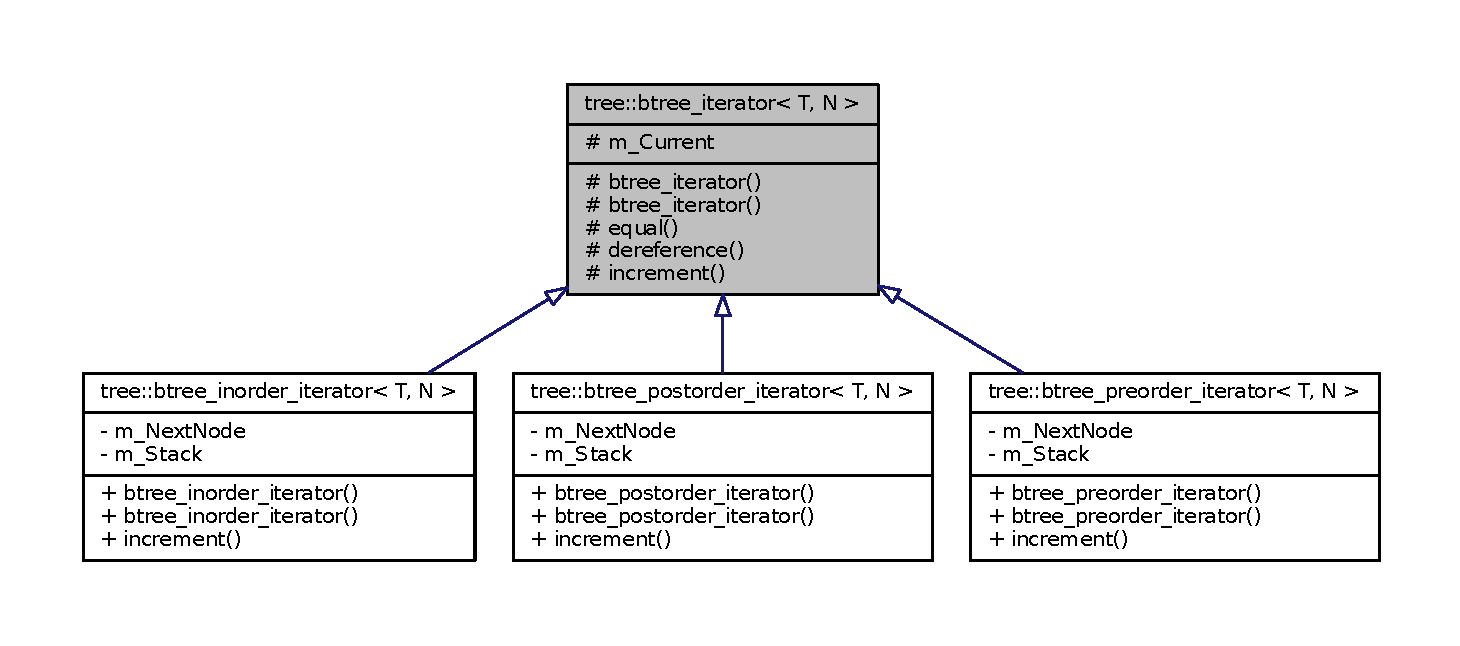
\includegraphics[width=350pt]{classtree_1_1btree__iterator__inherit__graph}
\end{center}
\end{figure}
\subsection*{\-Protected \-Member \-Functions}
\begin{DoxyCompactItemize}
\item 
\hypertarget{classtree_1_1btree__iterator_a9d7d63a542d5ed607bc93363080b247f}{{\bfseries btree\-\_\-iterator} (\-N $\ast$node)}\label{classtree_1_1btree__iterator_a9d7d63a542d5ed607bc93363080b247f}

\item 
\hypertarget{classtree_1_1btree__iterator_adaa03d21cddbb44f64abdfcfc92a15b4}{bool {\bfseries equal} (const \hyperlink{classtree_1_1btree__iterator}{btree\-\_\-iterator}$<$ \-T, \-N $>$ \&other) const }\label{classtree_1_1btree__iterator_adaa03d21cddbb44f64abdfcfc92a15b4}

\item 
\hypertarget{classtree_1_1btree__iterator_a2614a710559163bd7f8b8b9ea2998073}{\-T \& {\bfseries dereference} () const }\label{classtree_1_1btree__iterator_a2614a710559163bd7f8b8b9ea2998073}

\item 
\hypertarget{classtree_1_1btree__iterator_ac226882e50211134cae92e2d3a70a05a}{virtual void {\bfseries increment} ()}\label{classtree_1_1btree__iterator_ac226882e50211134cae92e2d3a70a05a}

\end{DoxyCompactItemize}
\subsection*{\-Protected \-Attributes}
\begin{DoxyCompactItemize}
\item 
\hypertarget{classtree_1_1btree__iterator_a3fe0a773310404a612dc9a46abfd5471}{\-N $\ast$ {\bfseries m\-\_\-\-Current}}\label{classtree_1_1btree__iterator_a3fe0a773310404a612dc9a46abfd5471}

\end{DoxyCompactItemize}
\subsection*{\-Friends}
\begin{DoxyCompactItemize}
\item 
\hypertarget{classtree_1_1btree__iterator_ac09f73e325921cc50ebcd96bed0f8096}{class {\bfseries boost\-::iterator\-\_\-core\-\_\-access}}\label{classtree_1_1btree__iterator_ac09f73e325921cc50ebcd96bed0f8096}

\item 
\hypertarget{classtree_1_1btree__iterator_a3bb2150f15bc37d06135e1e488e81e77}{class {\bfseries c\-Binary\-Rep}}\label{classtree_1_1btree__iterator_a3bb2150f15bc37d06135e1e488e81e77}

\end{DoxyCompactItemize}


\subsection{\-Detailed \-Description}
\subsubsection*{template$<$typename \-T, typename \-N$>$class tree\-::btree\-\_\-iterator$<$ T, N $>$}

binary tree iterator base class uses boost\-::iterator\-\_\-facade to implement the iterator 

\-The documentation for this class was generated from the following file\-:\begin{DoxyCompactItemize}
\item 
tree/binary\-\_\-tree\-\_\-iter.\-h\end{DoxyCompactItemize}

\hypertarget{classtree_1_1btree__iterator_3_01T_00_01btree__threaded__node_3_01T_01_4_01_4}{\section{tree\-:\-:btree\-\_\-iterator$<$ T, btree\-\_\-threaded\-\_\-node$<$ T $>$ $>$ Class Template Reference}
\label{classtree_1_1btree__iterator_3_01T_00_01btree__threaded__node_3_01T_01_4_01_4}\index{tree\-::btree\-\_\-iterator$<$ T, btree\-\_\-threaded\-\_\-node$<$ T $>$ $>$@{tree\-::btree\-\_\-iterator$<$ T, btree\-\_\-threaded\-\_\-node$<$ T $>$ $>$}}
}


partial specialization for iterators in a threaded binary tree representation///  




{\ttfamily \#include $<$binary\-\_\-tree\-\_\-iter.\-h$>$}



Inheritance diagram for tree\-:\-:btree\-\_\-iterator$<$ T, btree\-\_\-threaded\-\_\-node$<$ T $>$ $>$\-:
\nopagebreak
\begin{figure}[H]
\begin{center}
\leavevmode
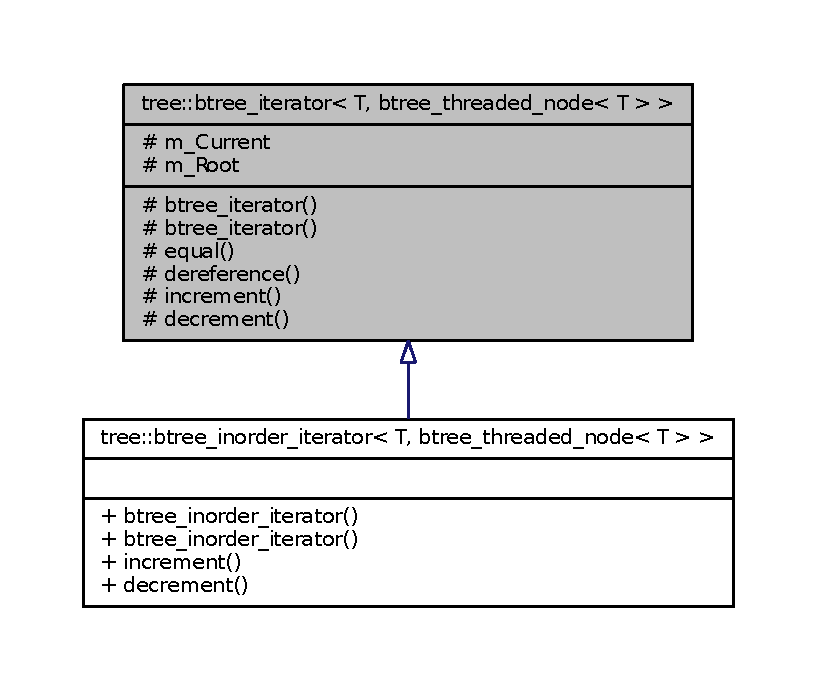
\includegraphics[width=262pt]{classtree_1_1btree__iterator_3_01T_00_01btree__threaded__node_3_01T_01_4_01_4__inherit__graph}
\end{center}
\end{figure}


Collaboration diagram for tree\-:\-:btree\-\_\-iterator$<$ T, btree\-\_\-threaded\-\_\-node$<$ T $>$ $>$\-:
\nopagebreak
\begin{figure}[H]
\begin{center}
\leavevmode
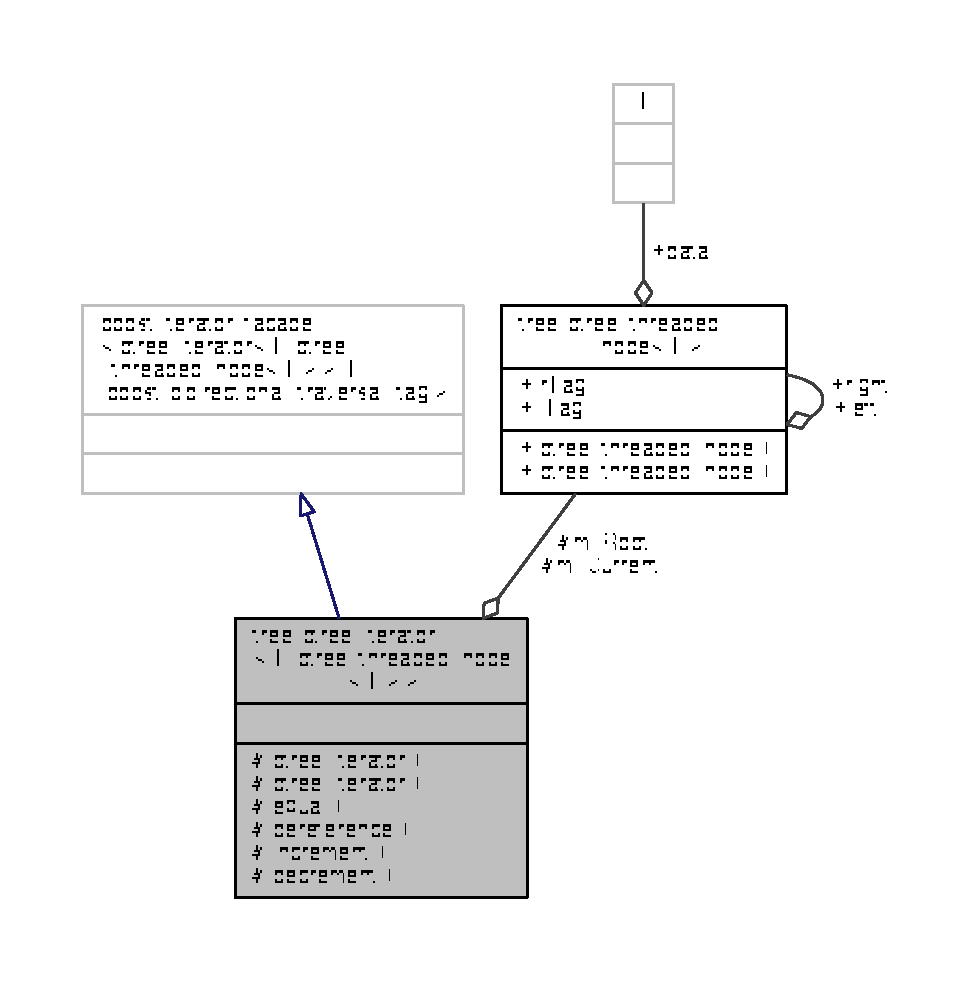
\includegraphics[width=350pt]{classtree_1_1btree__iterator_3_01T_00_01btree__threaded__node_3_01T_01_4_01_4__coll__graph}
\end{center}
\end{figure}
\subsection*{Protected Types}
\begin{DoxyCompactItemize}
\item 
\hypertarget{classtree_1_1btree__iterator_3_01T_00_01btree__threaded__node_3_01T_01_4_01_4_a4648c4864eba8e9052872c7d992a1114}{typedef \hyperlink{structtree_1_1btree__threaded__node}{btree\-\_\-threaded\-\_\-node}$<$ T $>$ {\bfseries N}}\label{classtree_1_1btree__iterator_3_01T_00_01btree__threaded__node_3_01T_01_4_01_4_a4648c4864eba8e9052872c7d992a1114}

\end{DoxyCompactItemize}
\subsection*{Protected Member Functions}
\begin{DoxyCompactItemize}
\item 
\hypertarget{classtree_1_1btree__iterator_3_01T_00_01btree__threaded__node_3_01T_01_4_01_4_a640a000899f88eeb630efd72d094e9a7}{{\bfseries btree\-\_\-iterator} (\hyperlink{structtree_1_1btree__threaded__node}{N} $\ast$node, \hyperlink{structtree_1_1btree__threaded__node}{N} $\ast$root)}\label{classtree_1_1btree__iterator_3_01T_00_01btree__threaded__node_3_01T_01_4_01_4_a640a000899f88eeb630efd72d094e9a7}

\item 
\hypertarget{classtree_1_1btree__iterator_3_01T_00_01btree__threaded__node_3_01T_01_4_01_4_a58d5ff373ab261c2e19b61356c959aa3}{bool {\bfseries equal} (const \hyperlink{classtree_1_1btree__iterator}{btree\-\_\-iterator}$<$ T, \hyperlink{structtree_1_1btree__threaded__node}{N} $>$ \&other) const }\label{classtree_1_1btree__iterator_3_01T_00_01btree__threaded__node_3_01T_01_4_01_4_a58d5ff373ab261c2e19b61356c959aa3}

\item 
\hypertarget{classtree_1_1btree__iterator_3_01T_00_01btree__threaded__node_3_01T_01_4_01_4_a79f975e8236e6bc9f5567897da84b874}{T \& {\bfseries dereference} () const }\label{classtree_1_1btree__iterator_3_01T_00_01btree__threaded__node_3_01T_01_4_01_4_a79f975e8236e6bc9f5567897da84b874}

\item 
\hypertarget{classtree_1_1btree__iterator_3_01T_00_01btree__threaded__node_3_01T_01_4_01_4_a05c30c85486c0429b543b1de8353b784}{virtual void {\bfseries increment} ()}\label{classtree_1_1btree__iterator_3_01T_00_01btree__threaded__node_3_01T_01_4_01_4_a05c30c85486c0429b543b1de8353b784}

\item 
\hypertarget{classtree_1_1btree__iterator_3_01T_00_01btree__threaded__node_3_01T_01_4_01_4_aea618d827646c2dc88f6aaed6076485c}{virtual void {\bfseries decrement} ()}\label{classtree_1_1btree__iterator_3_01T_00_01btree__threaded__node_3_01T_01_4_01_4_aea618d827646c2dc88f6aaed6076485c}

\end{DoxyCompactItemize}
\subsection*{Protected Attributes}
\begin{DoxyCompactItemize}
\item 
\hypertarget{classtree_1_1btree__iterator_3_01T_00_01btree__threaded__node_3_01T_01_4_01_4_a95443920e3a32b37c162c69cd41e6c96}{\hyperlink{structtree_1_1btree__threaded__node}{N} $\ast$ {\bfseries m\-\_\-\-Current}}\label{classtree_1_1btree__iterator_3_01T_00_01btree__threaded__node_3_01T_01_4_01_4_a95443920e3a32b37c162c69cd41e6c96}

\item 
\hypertarget{classtree_1_1btree__iterator_3_01T_00_01btree__threaded__node_3_01T_01_4_01_4_a8be171dbc88d3daf451dee7d7b969bf3}{\hyperlink{structtree_1_1btree__threaded__node}{N} $\ast$ {\bfseries m\-\_\-\-Root}}\label{classtree_1_1btree__iterator_3_01T_00_01btree__threaded__node_3_01T_01_4_01_4_a8be171dbc88d3daf451dee7d7b969bf3}

\end{DoxyCompactItemize}
\subsection*{Friends}
\begin{DoxyCompactItemize}
\item 
\hypertarget{classtree_1_1btree__iterator_3_01T_00_01btree__threaded__node_3_01T_01_4_01_4_ac09f73e325921cc50ebcd96bed0f8096}{class {\bfseries boost\-::iterator\-\_\-core\-\_\-access}}\label{classtree_1_1btree__iterator_3_01T_00_01btree__threaded__node_3_01T_01_4_01_4_ac09f73e325921cc50ebcd96bed0f8096}

\item 
\hypertarget{classtree_1_1btree__iterator_3_01T_00_01btree__threaded__node_3_01T_01_4_01_4_aaa5ba4484341fef93d9f0f42304b1290}{{\footnotesize template$<$typename $>$ }\\class {\bfseries c\-Threaded\-Rep}}\label{classtree_1_1btree__iterator_3_01T_00_01btree__threaded__node_3_01T_01_4_01_4_aaa5ba4484341fef93d9f0f42304b1290}

\end{DoxyCompactItemize}


\subsection{Detailed Description}
\subsubsection*{template$<$typename T$>$class tree\-::btree\-\_\-iterator$<$ T, btree\-\_\-threaded\-\_\-node$<$ T $>$ $>$}

partial specialization for iterators in a threaded binary tree representation/// 

binary tree iterator base class uses boost\-::iterator\-\_\-facade to implement the iterator !the threaded tree iterators are bidirectional 

The documentation for this class was generated from the following file\-:\begin{DoxyCompactItemize}
\item 
tree/binary\-\_\-tree\-\_\-iter.\-h\end{DoxyCompactItemize}

\hypertarget{structtree_1_1btree__node}{\section{tree\-:\-:btree\-\_\-node$<$ T $>$ Struct Template Reference}
\label{structtree_1_1btree__node}\index{tree\-::btree\-\_\-node$<$ T $>$@{tree\-::btree\-\_\-node$<$ T $>$}}
}


{\ttfamily \#include $<$tree\-\_\-common.\-h$>$}



Collaboration diagram for tree\-:\-:btree\-\_\-node$<$ T $>$\-:
\nopagebreak
\begin{figure}[H]
\begin{center}
\leavevmode
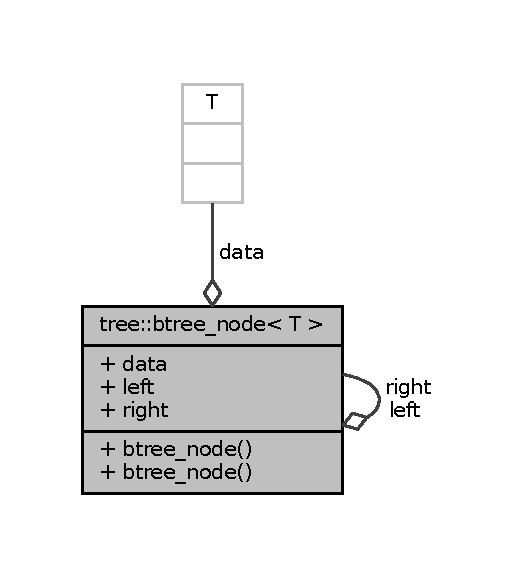
\includegraphics[width=247pt]{structtree_1_1btree__node__coll__graph}
\end{center}
\end{figure}
\subsection*{Public Member Functions}
\begin{DoxyCompactItemize}
\item 
\hypertarget{structtree_1_1btree__node_a6f97b71a8cb5cf273cf3a1635a1b8551}{{\bfseries btree\-\_\-node} (const T \&\-\_\-data)}\label{structtree_1_1btree__node_a6f97b71a8cb5cf273cf3a1635a1b8551}

\end{DoxyCompactItemize}
\subsection*{Public Attributes}
\begin{DoxyCompactItemize}
\item 
\hypertarget{structtree_1_1btree__node_a1f44c7c53c16a4f8827b0f4b468d4531}{T {\bfseries data}}\label{structtree_1_1btree__node_a1f44c7c53c16a4f8827b0f4b468d4531}

\item 
\hypertarget{structtree_1_1btree__node_aed5a80dfa830209910c13f7a55b91b83}{\hyperlink{structtree_1_1btree__node}{btree\-\_\-node} $\ast$ {\bfseries left}}\label{structtree_1_1btree__node_aed5a80dfa830209910c13f7a55b91b83}

\item 
\hypertarget{structtree_1_1btree__node_a82e9a7410832850bc4c05a5eb63fab21}{\hyperlink{structtree_1_1btree__node}{btree\-\_\-node} $\ast$ {\bfseries right}}\label{structtree_1_1btree__node_a82e9a7410832850bc4c05a5eb63fab21}

\end{DoxyCompactItemize}


\subsection{Detailed Description}
\subsubsection*{template$<$typename T$>$struct tree\-::btree\-\_\-node$<$ T $>$}

node type used by the binary tree internally 

The documentation for this struct was generated from the following file\-:\begin{DoxyCompactItemize}
\item 
tree/tree\-\_\-common.\-h\end{DoxyCompactItemize}

\hypertarget{classtree_1_1btree__postorder__iterator}{\section{tree\-:\-:btree\-\_\-postorder\-\_\-iterator$<$ \-T, \-N $>$ \-Class \-Template \-Reference}
\label{classtree_1_1btree__postorder__iterator}\index{tree\-::btree\-\_\-postorder\-\_\-iterator$<$ T, N $>$@{tree\-::btree\-\_\-postorder\-\_\-iterator$<$ T, N $>$}}
}


{\ttfamily \#include $<$binary\-\_\-tree\-\_\-iter.\-h$>$}



\-Inheritance diagram for tree\-:\-:btree\-\_\-postorder\-\_\-iterator$<$ \-T, \-N $>$\-:
\nopagebreak
\begin{figure}[H]
\begin{center}
\leavevmode
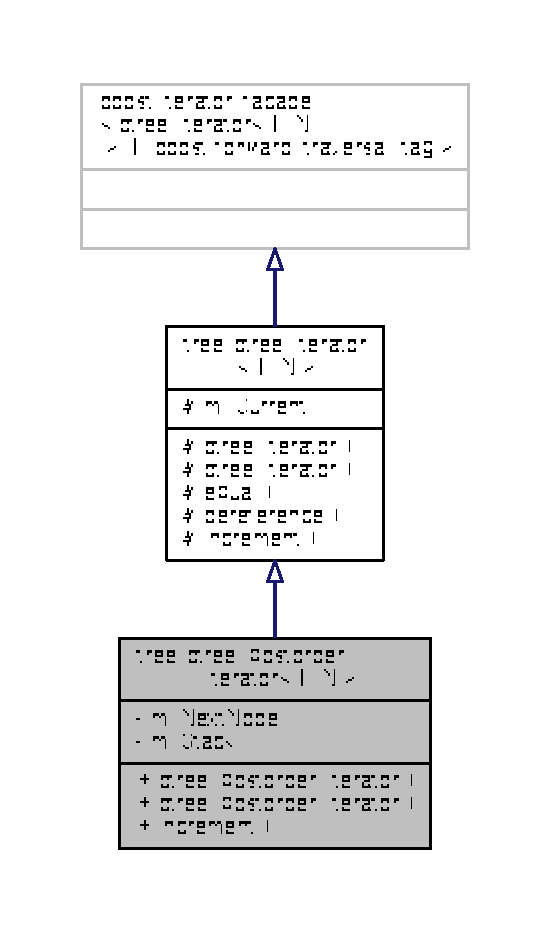
\includegraphics[width=280pt]{classtree_1_1btree__postorder__iterator__inherit__graph}
\end{center}
\end{figure}


\-Collaboration diagram for tree\-:\-:btree\-\_\-postorder\-\_\-iterator$<$ \-T, \-N $>$\-:
\nopagebreak
\begin{figure}[H]
\begin{center}
\leavevmode
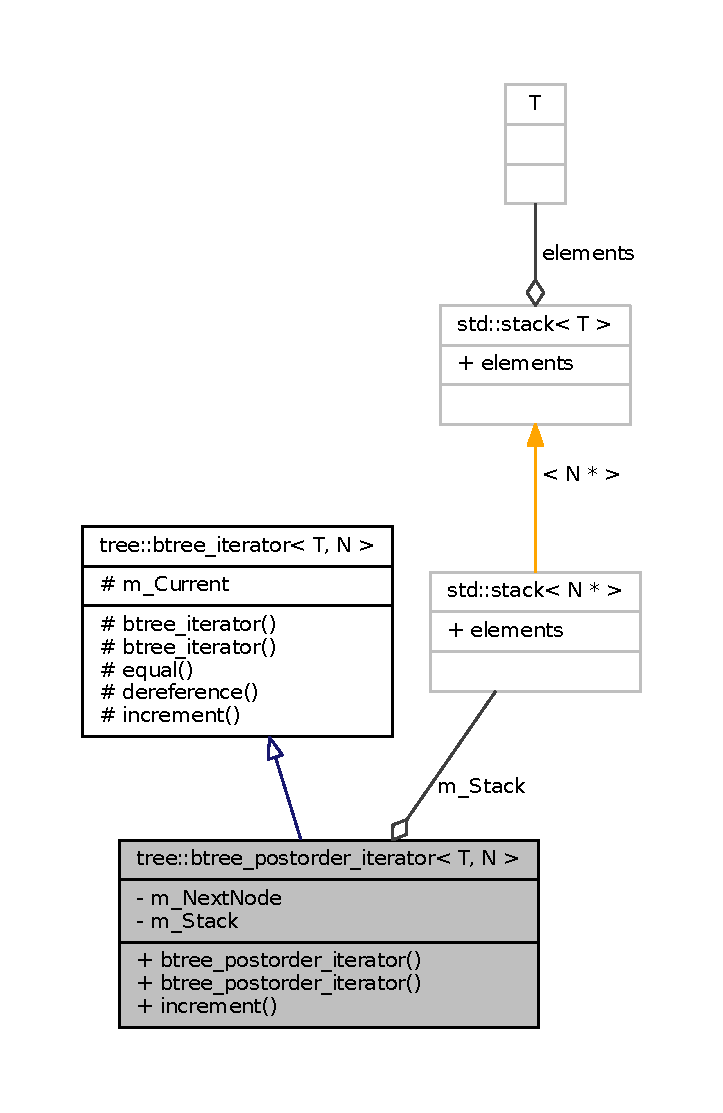
\includegraphics[width=347pt]{classtree_1_1btree__postorder__iterator__coll__graph}
\end{center}
\end{figure}
\subsection*{\-Public \-Member \-Functions}
\begin{DoxyCompactItemize}
\item 
\hypertarget{classtree_1_1btree__postorder__iterator_a9dec1c88cc657e81f3579058beda85b1}{{\bfseries btree\-\_\-postorder\-\_\-iterator} (\-N $\ast$node)}\label{classtree_1_1btree__postorder__iterator_a9dec1c88cc657e81f3579058beda85b1}

\item 
\hypertarget{classtree_1_1btree__postorder__iterator_ab4fb98322432ec53accacd76d17d520e}{void {\bfseries increment} ()}\label{classtree_1_1btree__postorder__iterator_ab4fb98322432ec53accacd76d17d520e}

\end{DoxyCompactItemize}
\subsection*{\-Private \-Attributes}
\begin{DoxyCompactItemize}
\item 
\hypertarget{classtree_1_1btree__postorder__iterator_afdbf2d545eae73723f0d93caa427cb85}{\-N $\ast$ {\bfseries m\-\_\-\-Next\-Node}}\label{classtree_1_1btree__postorder__iterator_afdbf2d545eae73723f0d93caa427cb85}

\item 
\hypertarget{classtree_1_1btree__postorder__iterator_a696bd97e9f2496b7a0ea95867fe87dc2}{std\-::stack$<$ \-N $\ast$ $>$ {\bfseries m\-\_\-\-Stack}}\label{classtree_1_1btree__postorder__iterator_a696bd97e9f2496b7a0ea95867fe87dc2}

\end{DoxyCompactItemize}


\subsection{\-Detailed \-Description}
\subsubsection*{template$<$typename T, typename N$>$class tree\-::btree\-\_\-postorder\-\_\-iterator$<$ T, N $>$}

traverses the tree in postorder(left, right, root) using a stack 

\-The documentation for this class was generated from the following file\-:\begin{DoxyCompactItemize}
\item 
tree/binary\-\_\-tree\-\_\-iter.\-h\end{DoxyCompactItemize}

\hypertarget{classtree_1_1btree__preorder__iterator}{\section{tree\-:\-:btree\-\_\-preorder\-\_\-iterator$<$ T, N $>$ Class Template Reference}
\label{classtree_1_1btree__preorder__iterator}\index{tree\-::btree\-\_\-preorder\-\_\-iterator$<$ T, N $>$@{tree\-::btree\-\_\-preorder\-\_\-iterator$<$ T, N $>$}}
}


{\ttfamily \#include $<$binary\-\_\-tree\-\_\-iter.\-h$>$}



Inheritance diagram for tree\-:\-:btree\-\_\-preorder\-\_\-iterator$<$ T, N $>$\-:


Collaboration diagram for tree\-:\-:btree\-\_\-preorder\-\_\-iterator$<$ T, N $>$\-:
\subsection*{Public Member Functions}
\begin{DoxyCompactItemize}
\item 
\hypertarget{classtree_1_1btree__preorder__iterator_a2d2e4be80bd9f420f209465b595fb146}{{\bfseries btree\-\_\-preorder\-\_\-iterator} (N $\ast$node)}\label{classtree_1_1btree__preorder__iterator_a2d2e4be80bd9f420f209465b595fb146}

\item 
\hypertarget{classtree_1_1btree__preorder__iterator_afa601bda88a4be48f38d6438260f0001}{void {\bfseries increment} ()}\label{classtree_1_1btree__preorder__iterator_afa601bda88a4be48f38d6438260f0001}

\end{DoxyCompactItemize}
\subsection*{Private Attributes}
\begin{DoxyCompactItemize}
\item 
\hypertarget{classtree_1_1btree__preorder__iterator_a142dc25e4c41f10c96cc738182d2eb18}{N $\ast$ {\bfseries m\-\_\-\-Next\-Node}}\label{classtree_1_1btree__preorder__iterator_a142dc25e4c41f10c96cc738182d2eb18}

\item 
\hypertarget{classtree_1_1btree__preorder__iterator_a790df750993384cb0c3056c0dd780cc0}{std\-::stack$<$ N $\ast$ $>$ {\bfseries m\-\_\-\-Stack}}\label{classtree_1_1btree__preorder__iterator_a790df750993384cb0c3056c0dd780cc0}

\end{DoxyCompactItemize}
\subsection*{Additional Inherited Members}


\subsection{Detailed Description}
\subsubsection*{template$<$typename T, typename N$>$class tree\-::btree\-\_\-preorder\-\_\-iterator$<$ T, N $>$}

traverses the tree in preorder(root, left, right) using a stack 

The documentation for this class was generated from the following file\-:\begin{DoxyCompactItemize}
\item 
tree/binary\-\_\-tree\-\_\-iter.\-h\end{DoxyCompactItemize}

\hypertarget{structtree_1_1btree__threaded__node}{\section{tree\-:\-:btree\-\_\-threaded\-\_\-node$<$ \-T $>$ \-Struct \-Template \-Reference}
\label{structtree_1_1btree__threaded__node}\index{tree\-::btree\-\_\-threaded\-\_\-node$<$ T $>$@{tree\-::btree\-\_\-threaded\-\_\-node$<$ T $>$}}
}


{\ttfamily \#include $<$tree\-\_\-common.\-h$>$}



\-Collaboration diagram for tree\-:\-:btree\-\_\-threaded\-\_\-node$<$ \-T $>$\-:
\nopagebreak
\begin{figure}[H]
\begin{center}
\leavevmode
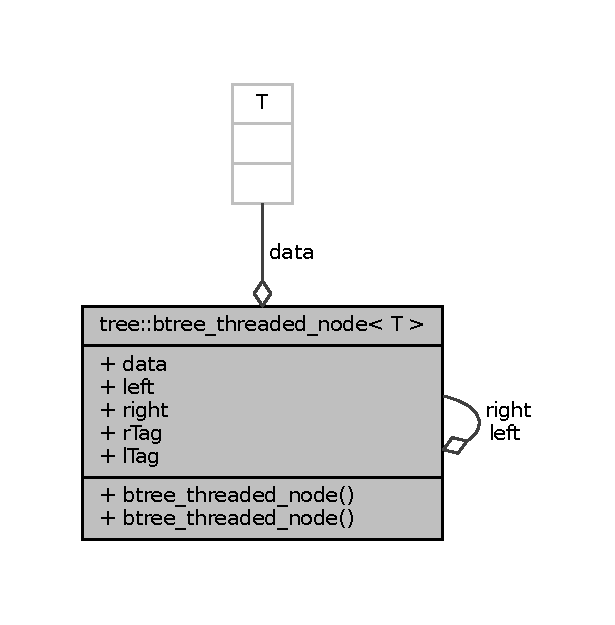
\includegraphics[width=295pt]{structtree_1_1btree__threaded__node__coll__graph}
\end{center}
\end{figure}
\subsection*{\-Public \-Member \-Functions}
\begin{DoxyCompactItemize}
\item 
\hypertarget{structtree_1_1btree__threaded__node_a2752127b5320f35b87cd1e347db586f5}{{\bfseries btree\-\_\-threaded\-\_\-node} (const \-T \&\-\_\-data)}\label{structtree_1_1btree__threaded__node_a2752127b5320f35b87cd1e347db586f5}

\end{DoxyCompactItemize}
\subsection*{\-Public \-Attributes}
\begin{DoxyCompactItemize}
\item 
\hypertarget{structtree_1_1btree__threaded__node_a4eedf9c4f0d905ca2163d37ddcb855be}{\-T {\bfseries data}}\label{structtree_1_1btree__threaded__node_a4eedf9c4f0d905ca2163d37ddcb855be}

\item 
\hypertarget{structtree_1_1btree__threaded__node_ae2f6a8e3479fc61c5cd635a649a2b0f0}{\hyperlink{structtree_1_1btree__threaded__node}{btree\-\_\-threaded\-\_\-node} $\ast$ {\bfseries left}}\label{structtree_1_1btree__threaded__node_ae2f6a8e3479fc61c5cd635a649a2b0f0}

\item 
\hypertarget{structtree_1_1btree__threaded__node_ad2ffcfc42ad38e941223e32995013b21}{\hyperlink{structtree_1_1btree__threaded__node}{btree\-\_\-threaded\-\_\-node} $\ast$ {\bfseries right}}\label{structtree_1_1btree__threaded__node_ad2ffcfc42ad38e941223e32995013b21}

\item 
\hypertarget{structtree_1_1btree__threaded__node_a06b2ebcf5e85dd9feb184872af4a6e30}{bool {\bfseries r\-Tag}}\label{structtree_1_1btree__threaded__node_a06b2ebcf5e85dd9feb184872af4a6e30}

\item 
\hypertarget{structtree_1_1btree__threaded__node_a1179a89253389e3c964653739394fbbd}{bool {\bfseries l\-Tag}}\label{structtree_1_1btree__threaded__node_a1179a89253389e3c964653739394fbbd}

\end{DoxyCompactItemize}


\subsection{\-Detailed \-Description}
\subsubsection*{template$<$typename T$>$struct tree\-::btree\-\_\-threaded\-\_\-node$<$ T $>$}

node type used by the binary tree threaded representation r\-Tag = false -\/$>$ right points to child r\-Tag = true -\/$>$ right points to the inorder predecesor l\-Tag = false -\/$>$ left points to a child l\-Tag = true -\/$>$ left points to the inorder successor 

\-The documentation for this struct was generated from the following file\-:\begin{DoxyCompactItemize}
\item 
tree/tree\-\_\-common.\-h\end{DoxyCompactItemize}

\hypertarget{classtree_1_1cBinaryRep}{\section{tree\-:\-:c\-Binary\-Rep$<$ T $>$ Class Template Reference}
\label{classtree_1_1cBinaryRep}\index{tree\-::c\-Binary\-Rep$<$ T $>$@{tree\-::c\-Binary\-Rep$<$ T $>$}}
}


{\ttfamily \#include $<$binary\-\_\-rep.\-h$>$}



Collaboration diagram for tree\-:\-:c\-Binary\-Rep$<$ T $>$\-:
\nopagebreak
\begin{figure}[H]
\begin{center}
\leavevmode
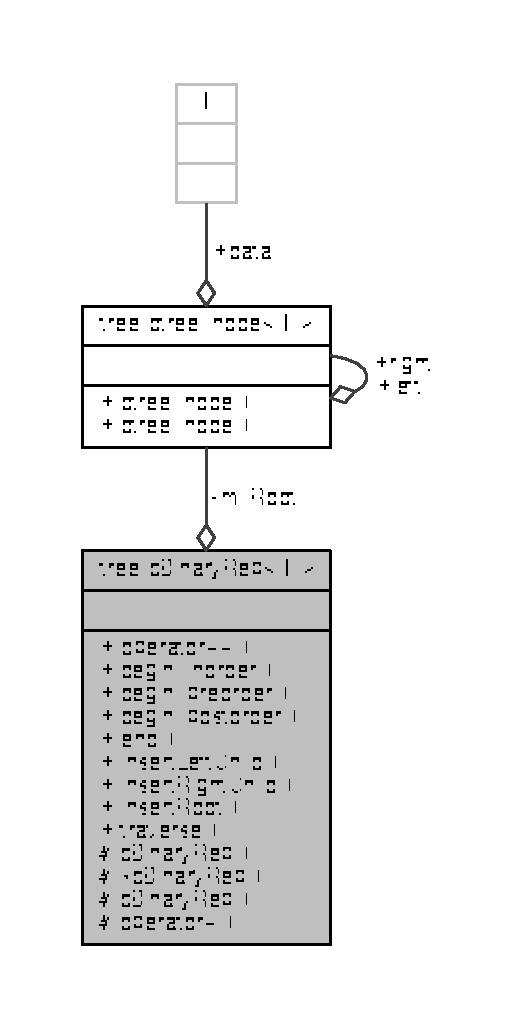
\includegraphics[width=247pt]{classtree_1_1cBinaryRep__coll__graph}
\end{center}
\end{figure}
\subsection*{Public Types}
\begin{DoxyCompactItemize}
\item 
\hypertarget{classtree_1_1cBinaryRep_a4218118406b4b792f771f2cffab1fe67}{typedef \hyperlink{structtree_1_1btree__node}{btree\-\_\-node}$<$ T $>$ {\bfseries node\-\_\-type}}\label{classtree_1_1cBinaryRep_a4218118406b4b792f771f2cffab1fe67}

\item 
\hypertarget{classtree_1_1cBinaryRep_af8646ca9dd6c8e2abc30f0a24eea2785}{typedef \hyperlink{classtree_1_1btree__iterator}{btree\-\_\-iterator}$<$ T, \\*
\hyperlink{structtree_1_1btree__node}{node\-\_\-type} $>$ {\bfseries iterator}}\label{classtree_1_1cBinaryRep_af8646ca9dd6c8e2abc30f0a24eea2785}

\item 
\hypertarget{classtree_1_1cBinaryRep_a80d54fe0461119770e3be144672dcbc6}{typedef \\*
\hyperlink{classtree_1_1btree__preorder__iterator}{btree\-\_\-preorder\-\_\-iterator}$<$ T, \\*
\hyperlink{structtree_1_1btree__node}{node\-\_\-type} $>$ {\bfseries preorder\-\_\-iterator}}\label{classtree_1_1cBinaryRep_a80d54fe0461119770e3be144672dcbc6}

\item 
\hypertarget{classtree_1_1cBinaryRep_ad1bba7a7672ee7bdf7ef4979a1b00879}{typedef \hyperlink{classtree_1_1btree__inorder__iterator}{btree\-\_\-inorder\-\_\-iterator}\\*
$<$ T, \hyperlink{structtree_1_1btree__node}{node\-\_\-type} $>$ {\bfseries inorder\-\_\-iterator}}\label{classtree_1_1cBinaryRep_ad1bba7a7672ee7bdf7ef4979a1b00879}

\item 
\hypertarget{classtree_1_1cBinaryRep_a7bef52fb6be8078a9d082c22f9054dd0}{typedef \\*
\hyperlink{classtree_1_1btree__postorder__iterator}{btree\-\_\-postorder\-\_\-iterator}$<$ T, \\*
\hyperlink{structtree_1_1btree__node}{node\-\_\-type} $>$ {\bfseries postorder\-\_\-iterator}}\label{classtree_1_1cBinaryRep_a7bef52fb6be8078a9d082c22f9054dd0}

\end{DoxyCompactItemize}
\subsection*{Public Member Functions}
\begin{DoxyCompactItemize}
\item 
bool \hyperlink{classtree_1_1cBinaryRep_a7a8f861470cb8538aa03ddbb9cbac6af}{operator==} (const \hyperlink{classtree_1_1cBinaryRep}{c\-Binary\-Rep} \&bin\-\_\-rep)
\item 
\hyperlink{classtree_1_1btree__inorder__iterator}{inorder\-\_\-iterator} \hyperlink{classtree_1_1cBinaryRep_a5701848a04cd825236bc125b33e376d8}{begin\-\_\-inorder} ()
\item 
\hyperlink{classtree_1_1btree__preorder__iterator}{preorder\-\_\-iterator} \hyperlink{classtree_1_1cBinaryRep_a6e912be346d3626156df92eabecee012}{begin\-\_\-preorder} ()
\item 
\hyperlink{classtree_1_1btree__postorder__iterator}{postorder\-\_\-iterator} \hyperlink{classtree_1_1cBinaryRep_a99f4029023bc6b07fade450aceb2f17d}{begin\-\_\-postorder} ()
\item 
\hyperlink{classtree_1_1btree__preorder__iterator}{preorder\-\_\-iterator} \hyperlink{classtree_1_1cBinaryRep_acf645e7e2447eb801c71ac752ecede22}{end} ()
\item 
\hyperlink{classtree_1_1btree__iterator}{iterator} \hyperlink{classtree_1_1cBinaryRep_a1bd7a582b25b1f7a4ff76ea936377458}{insert\-Left\-Child} (\hyperlink{classtree_1_1btree__iterator}{iterator} iter, const T \&data)
\item 
\hyperlink{classtree_1_1btree__iterator}{iterator} \hyperlink{classtree_1_1cBinaryRep_a593596cea8e60e85a0f66fb3354617a8}{insert\-Right\-Child} (\hyperlink{classtree_1_1btree__iterator}{iterator} iter, const T \&data)
\item 
\hypertarget{classtree_1_1cBinaryRep_aae971b4e02baaa0c4d51ce1416ca2178}{\hyperlink{classtree_1_1btree__iterator}{iterator} {\bfseries insert\-Root} (const T \&data)}\label{classtree_1_1cBinaryRep_aae971b4e02baaa0c4d51ce1416ca2178}

\item 
{\footnotesize template$<$typename F\-U\-N\-C $>$ }\\void \hyperlink{classtree_1_1cBinaryRep_aebf973eb7334a5cf2134a51ebc519d33}{traverse} (tree\-\_\-traversal traversal, F\-U\-N\-C \&visit)
\end{DoxyCompactItemize}
\subsection*{Protected Member Functions}
\begin{DoxyCompactItemize}
\item 
\hypertarget{classtree_1_1cBinaryRep_a2b7e8d490a1e5f4b5c58fb58e29330ef}{{\bfseries c\-Binary\-Rep} (const \hyperlink{classtree_1_1cBinaryRep}{c\-Binary\-Rep} \&bin\-\_\-rep)}\label{classtree_1_1cBinaryRep_a2b7e8d490a1e5f4b5c58fb58e29330ef}

\item 
\hypertarget{classtree_1_1cBinaryRep_a4c6eb53e4805dcb0ac0032289bb7d0d8}{\hyperlink{classtree_1_1cBinaryRep}{c\-Binary\-Rep} \& {\bfseries operator=} (const \hyperlink{classtree_1_1cBinaryRep}{c\-Binary\-Rep} \&bin\-\_\-rep)}\label{classtree_1_1cBinaryRep_a4c6eb53e4805dcb0ac0032289bb7d0d8}

\end{DoxyCompactItemize}
\subsection*{Private Attributes}
\begin{DoxyCompactItemize}
\item 
\hypertarget{classtree_1_1cBinaryRep_acc04e77d74d4c7be7aceb048d512965a}{\hyperlink{structtree_1_1btree__node}{node\-\_\-type} $\ast$ {\bfseries m\-\_\-\-Root}}\label{classtree_1_1cBinaryRep_acc04e77d74d4c7be7aceb048d512965a}

\end{DoxyCompactItemize}


\subsection{Detailed Description}
\subsubsection*{template$<$typename T$>$class tree\-::c\-Binary\-Rep$<$ T $>$}

binary tree usual representation(left node pointing to the left subtree, right node pointing to the right subtree) 

\subsection{Member Function Documentation}
\hypertarget{classtree_1_1cBinaryRep_a5701848a04cd825236bc125b33e376d8}{\index{tree\-::c\-Binary\-Rep@{tree\-::c\-Binary\-Rep}!begin\-\_\-inorder@{begin\-\_\-inorder}}
\index{begin\-\_\-inorder@{begin\-\_\-inorder}!tree::cBinaryRep@{tree\-::c\-Binary\-Rep}}
\subsubsection[{begin\-\_\-inorder}]{\setlength{\rightskip}{0pt plus 5cm}template$<$typename T $>$ {\bf inorder\-\_\-iterator} {\bf tree\-::c\-Binary\-Rep}$<$ T $>$\-::begin\-\_\-inorder (
\begin{DoxyParamCaption}
{}
\end{DoxyParamCaption}
)\hspace{0.3cm}{\ttfamily [inline]}}}\label{classtree_1_1cBinaryRep_a5701848a04cd825236bc125b33e376d8}
returns an iterator to the beginning of the tree for inorder traversal \hypertarget{classtree_1_1cBinaryRep_a99f4029023bc6b07fade450aceb2f17d}{\index{tree\-::c\-Binary\-Rep@{tree\-::c\-Binary\-Rep}!begin\-\_\-postorder@{begin\-\_\-postorder}}
\index{begin\-\_\-postorder@{begin\-\_\-postorder}!tree::cBinaryRep@{tree\-::c\-Binary\-Rep}}
\subsubsection[{begin\-\_\-postorder}]{\setlength{\rightskip}{0pt plus 5cm}template$<$typename T $>$ {\bf postorder\-\_\-iterator} {\bf tree\-::c\-Binary\-Rep}$<$ T $>$\-::begin\-\_\-postorder (
\begin{DoxyParamCaption}
{}
\end{DoxyParamCaption}
)\hspace{0.3cm}{\ttfamily [inline]}}}\label{classtree_1_1cBinaryRep_a99f4029023bc6b07fade450aceb2f17d}
returns an iterator to the beginning of the tree for postorder traversal \hypertarget{classtree_1_1cBinaryRep_a6e912be346d3626156df92eabecee012}{\index{tree\-::c\-Binary\-Rep@{tree\-::c\-Binary\-Rep}!begin\-\_\-preorder@{begin\-\_\-preorder}}
\index{begin\-\_\-preorder@{begin\-\_\-preorder}!tree::cBinaryRep@{tree\-::c\-Binary\-Rep}}
\subsubsection[{begin\-\_\-preorder}]{\setlength{\rightskip}{0pt plus 5cm}template$<$typename T $>$ {\bf preorder\-\_\-iterator} {\bf tree\-::c\-Binary\-Rep}$<$ T $>$\-::begin\-\_\-preorder (
\begin{DoxyParamCaption}
{}
\end{DoxyParamCaption}
)\hspace{0.3cm}{\ttfamily [inline]}}}\label{classtree_1_1cBinaryRep_a6e912be346d3626156df92eabecee012}
returns an iterator to the beginning of the tree for preorder traversal \hypertarget{classtree_1_1cBinaryRep_acf645e7e2447eb801c71ac752ecede22}{\index{tree\-::c\-Binary\-Rep@{tree\-::c\-Binary\-Rep}!end@{end}}
\index{end@{end}!tree::cBinaryRep@{tree\-::c\-Binary\-Rep}}
\subsubsection[{end}]{\setlength{\rightskip}{0pt plus 5cm}template$<$typename T $>$ {\bf preorder\-\_\-iterator} {\bf tree\-::c\-Binary\-Rep}$<$ T $>$\-::end (
\begin{DoxyParamCaption}
{}
\end{DoxyParamCaption}
)\hspace{0.3cm}{\ttfamily [inline]}}}\label{classtree_1_1cBinaryRep_acf645e7e2447eb801c71ac752ecede22}
returns an empty iterator signifying the end of the tree ! used in constructs like for(iterator it = tree.\-begin(); it != tree.\-end(); it++) \hypertarget{classtree_1_1cBinaryRep_a1bd7a582b25b1f7a4ff76ea936377458}{\index{tree\-::c\-Binary\-Rep@{tree\-::c\-Binary\-Rep}!insert\-Left\-Child@{insert\-Left\-Child}}
\index{insert\-Left\-Child@{insert\-Left\-Child}!tree::cBinaryRep@{tree\-::c\-Binary\-Rep}}
\subsubsection[{insert\-Left\-Child}]{\setlength{\rightskip}{0pt plus 5cm}template$<$typename T $>$ {\bf iterator} {\bf tree\-::c\-Binary\-Rep}$<$ T $>$\-::insert\-Left\-Child (
\begin{DoxyParamCaption}
\item[{{\bf iterator}}]{iter, }
\item[{const T \&}]{data}
\end{DoxyParamCaption}
)\hspace{0.3cm}{\ttfamily [inline]}}}\label{classtree_1_1cBinaryRep_a1bd7a582b25b1f7a4ff76ea936377458}
inserts data as a left child of the node indicated by the iterator \hypertarget{classtree_1_1cBinaryRep_a593596cea8e60e85a0f66fb3354617a8}{\index{tree\-::c\-Binary\-Rep@{tree\-::c\-Binary\-Rep}!insert\-Right\-Child@{insert\-Right\-Child}}
\index{insert\-Right\-Child@{insert\-Right\-Child}!tree::cBinaryRep@{tree\-::c\-Binary\-Rep}}
\subsubsection[{insert\-Right\-Child}]{\setlength{\rightskip}{0pt plus 5cm}template$<$typename T $>$ {\bf iterator} {\bf tree\-::c\-Binary\-Rep}$<$ T $>$\-::insert\-Right\-Child (
\begin{DoxyParamCaption}
\item[{{\bf iterator}}]{iter, }
\item[{const T \&}]{data}
\end{DoxyParamCaption}
)\hspace{0.3cm}{\ttfamily [inline]}}}\label{classtree_1_1cBinaryRep_a593596cea8e60e85a0f66fb3354617a8}
inserts data as a right child of the node indicated by the iterator \hypertarget{classtree_1_1cBinaryRep_a7a8f861470cb8538aa03ddbb9cbac6af}{\index{tree\-::c\-Binary\-Rep@{tree\-::c\-Binary\-Rep}!operator==@{operator==}}
\index{operator==@{operator==}!tree::cBinaryRep@{tree\-::c\-Binary\-Rep}}
\subsubsection[{operator==}]{\setlength{\rightskip}{0pt plus 5cm}template$<$typename T $>$ bool {\bf tree\-::c\-Binary\-Rep}$<$ T $>$\-::operator== (
\begin{DoxyParamCaption}
\item[{const {\bf c\-Binary\-Rep}$<$ T $>$ \&}]{bin\-\_\-rep}
\end{DoxyParamCaption}
)\hspace{0.3cm}{\ttfamily [inline]}}}\label{classtree_1_1cBinaryRep_a7a8f861470cb8538aa03ddbb9cbac6af}
checks for equality -- !compares the data in every node of the tree for equality \hypertarget{classtree_1_1cBinaryRep_aebf973eb7334a5cf2134a51ebc519d33}{\index{tree\-::c\-Binary\-Rep@{tree\-::c\-Binary\-Rep}!traverse@{traverse}}
\index{traverse@{traverse}!tree::cBinaryRep@{tree\-::c\-Binary\-Rep}}
\subsubsection[{traverse}]{\setlength{\rightskip}{0pt plus 5cm}template$<$typename T $>$ template$<$typename F\-U\-N\-C $>$ void {\bf tree\-::c\-Binary\-Rep}$<$ T $>$\-::traverse (
\begin{DoxyParamCaption}
\item[{tree\-\_\-traversal}]{traversal, }
\item[{F\-U\-N\-C \&}]{visit}
\end{DoxyParamCaption}
)\hspace{0.3cm}{\ttfamily [inline]}}}\label{classtree_1_1cBinaryRep_aebf973eb7334a5cf2134a51ebc519d33}
traverse the binary tree in the given tree\-\_\-traversal order takes a function object as a parameter, which must implement operator(\-T) 

The documentation for this class was generated from the following file\-:\begin{DoxyCompactItemize}
\item 
tree/binary\-\_\-rep.\-h\end{DoxyCompactItemize}

\hypertarget{classtree_1_1cBinaryTree}{\section{tree\-:\-:c\-Binary\-Tree$<$ T, R\-E\-P $>$ Class Template Reference}
\label{classtree_1_1cBinaryTree}\index{tree\-::c\-Binary\-Tree$<$ T, R\-E\-P $>$@{tree\-::c\-Binary\-Tree$<$ T, R\-E\-P $>$}}
}


{\ttfamily \#include $<$binary\-\_\-tree.\-h$>$}



Collaboration diagram for tree\-:\-:c\-Binary\-Tree$<$ T, R\-E\-P $>$\-:


\subsection{Detailed Description}
\subsubsection*{template$<$typename T, template$<$ typename $>$ class R\-E\-P$>$class tree\-::c\-Binary\-Tree$<$ T, R\-E\-P $>$}

class that represents a binary tree (interface common to all binary tree representations\-: binary\-\_\-rep, threaded\-\_\-rep) 

The documentation for this class was generated from the following file\-:\begin{DoxyCompactItemize}
\item 
tree/binary\-\_\-tree.\-h\end{DoxyCompactItemize}

\hypertarget{classcCayleyGrf}{\section{c\-Cayley\-Grf$<$ \-G $>$ \-Class \-Template \-Reference}
\label{classcCayleyGrf}\index{c\-Cayley\-Grf$<$ G $>$@{c\-Cayley\-Grf$<$ G $>$}}
}


{\ttfamily \#include $<$cayley\-\_\-graph.\-h$>$}



\-Collaboration diagram for c\-Cayley\-Grf$<$ \-G $>$\-:\nopagebreak
\begin{figure}[H]
\begin{center}
\leavevmode
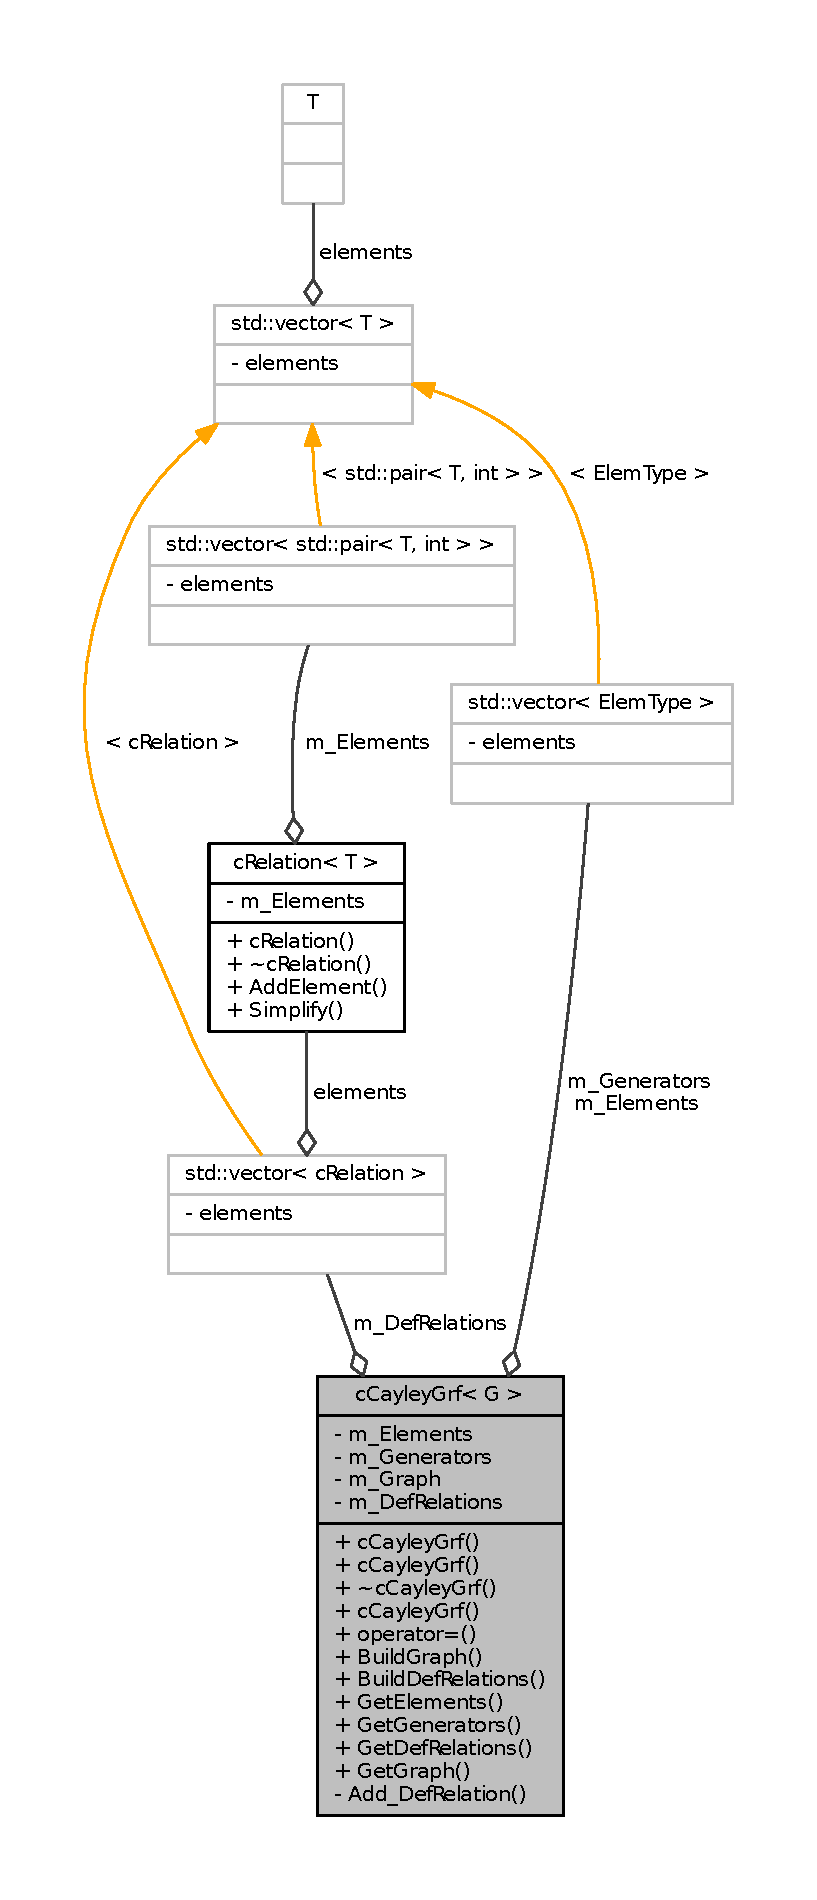
\includegraphics[height=550pt]{classcCayleyGrf__coll__graph}
\end{center}
\end{figure}
\subsection*{\-Classes}
\begin{DoxyCompactItemize}
\item 
class \hyperlink{classcCayleyGrf_1_1cColourEdgesVis}{c\-Colour\-Edges\-Vis}
\end{DoxyCompactItemize}
\subsection*{\-Public \-Types}
\begin{DoxyCompactItemize}
\item 
\hypertarget{classcCayleyGrf_a96e2347884f970817ad4f941ff85f478}{typedef \-G\-::\-Element\-Type {\bfseries \-Elem\-Type}}\label{classcCayleyGrf_a96e2347884f970817ad4f941ff85f478}

\item 
\hypertarget{classcCayleyGrf_aa6ec3ba98e73a5c244786d88e05dc380}{typedef boost\-::adjacency\-\_\-list\*
$<$ boost\-::list\-S, boost\-::vec\-S, \*
boost\-::directed\-S, \-Elem\-Type, \*
std\-::pair$<$ \-Elem\-Type, bool $>$ $>$ {\bfseries \-Graph}}\label{classcCayleyGrf_aa6ec3ba98e73a5c244786d88e05dc380}

\item 
\hypertarget{classcCayleyGrf_a1ef27f6e825137691b820322094745b3}{typedef boost\-::graph\-\_\-traits\*
$<$ \-Graph $>$\-::vertex\-\_\-descriptor {\bfseries \-Vertex}}\label{classcCayleyGrf_a1ef27f6e825137691b820322094745b3}

\item 
\hypertarget{classcCayleyGrf_abade7422415758e7d2699ccfa052accb}{typedef boost\-::graph\-\_\-traits\*
$<$ \-Graph $>$\-::edge\-\_\-descriptor {\bfseries \-Edge}}\label{classcCayleyGrf_abade7422415758e7d2699ccfa052accb}

\item 
\hypertarget{classcCayleyGrf_a8a2a9d7e45de509f97daf663b6827496}{typedef boost\-::graph\-\_\-traits\*
$<$ \-Graph $>$\-::vertex\-\_\-iterator {\bfseries \-Vertex\-Iterator}}\label{classcCayleyGrf_a8a2a9d7e45de509f97daf663b6827496}

\end{DoxyCompactItemize}
\subsection*{\-Public \-Member \-Functions}
\begin{DoxyCompactItemize}
\item 
\hypertarget{classcCayleyGrf_ac94c0ddf2262aab4ce17454fb10e7286}{{\bfseries c\-Cayley\-Grf} (std\-::vector$<$ \-Elem\-Type $>$ \&elements, std\-::vector$<$ \-Elem\-Type $>$ \&generators)}\label{classcCayleyGrf_ac94c0ddf2262aab4ce17454fb10e7286}

\item 
\hypertarget{classcCayleyGrf_a6f1bc787dd952aae0b5e5d4d6d39fe35}{{\bfseries c\-Cayley\-Grf} (\-G \&group)}\label{classcCayleyGrf_a6f1bc787dd952aae0b5e5d4d6d39fe35}

\item 
\hypertarget{classcCayleyGrf_ae597aa2fce821346c6f3976e70eb6a75}{{\bfseries c\-Cayley\-Grf} (const \hyperlink{classcCayleyGrf}{c\-Cayley\-Grf} \&graph)}\label{classcCayleyGrf_ae597aa2fce821346c6f3976e70eb6a75}

\item 
\hypertarget{classcCayleyGrf_a31a02f7a0e7702fe953409f7f82888be}{\hyperlink{classcCayleyGrf}{c\-Cayley\-Grf} \& {\bfseries operator=} (const \hyperlink{classcCayleyGrf}{c\-Cayley\-Grf} \&graph)}\label{classcCayleyGrf_a31a02f7a0e7702fe953409f7f82888be}

\item 
void \hyperlink{classcCayleyGrf_a4a0ff02aa7bb9d556456b34e9f66f3d9}{\-Build\-Graph} ()
\item 
void \hyperlink{classcCayleyGrf_a8517436f6101a294fa7f30355efaa196}{\-Build\-Def\-Relations} ()
\item 
\hypertarget{classcCayleyGrf_a77314418cd7c7e09f5ed92db3fb77b6f}{const std\-::vector\*
$<$ \hyperlink{classcGroupRelation}{c\-Group\-Relation}$<$ \-Elem\-Type $>$ $>$ \& {\bfseries \-Get\-Def\-Relations} () const }\label{classcCayleyGrf_a77314418cd7c7e09f5ed92db3fb77b6f}

\item 
\-Graph $\ast$ \hyperlink{classcCayleyGrf_aeb4d8533b65921ca63fdaaf4516f92f6}{\-Get\-Graph} () const 
\end{DoxyCompactItemize}
\subsection*{\-Private \-Member \-Functions}
\begin{DoxyCompactItemize}
\item 
void \hyperlink{classcCayleyGrf_a5aef2537b624f06052dc852890b37048}{\-Add\-\_\-\-Def\-Relation} (const \-Edge \&edge)
\end{DoxyCompactItemize}
\subsection*{\-Private \-Attributes}
\begin{DoxyCompactItemize}
\item 
\hypertarget{classcCayleyGrf_af4c3fa359332e9097ad511da6df21e01}{std\-::vector$<$ \-Elem\-Type $>$ {\bfseries m\-\_\-\-Elements}}\label{classcCayleyGrf_af4c3fa359332e9097ad511da6df21e01}

\item 
\hypertarget{classcCayleyGrf_aa0263f38d2605e8b1c43830af0dd7d9b}{std\-::vector$<$ \-Elem\-Type $>$ {\bfseries m\-\_\-\-Generators}}\label{classcCayleyGrf_aa0263f38d2605e8b1c43830af0dd7d9b}

\item 
\hypertarget{classcCayleyGrf_a8ac7f5226ca5868bfb9bbfbd10021981}{\-Graph $\ast$ {\bfseries m\-\_\-\-Graph}}\label{classcCayleyGrf_a8ac7f5226ca5868bfb9bbfbd10021981}

\item 
\hypertarget{classcCayleyGrf_add18aca50d8b803c016d9a8990472a57}{std\-::vector$<$ \hyperlink{classcGroupRelation}{c\-Group\-Relation}\*
$<$ \-Elem\-Type $>$ $>$ {\bfseries m\-\_\-\-Def\-Relations}}\label{classcCayleyGrf_add18aca50d8b803c016d9a8990472a57}

\end{DoxyCompactItemize}
\subsection*{\-Friends}
\begin{DoxyCompactItemize}
\item 
\hypertarget{classcCayleyGrf_a335728ff704ed565af614d4eadbc4609}{std\-::ostream \& {\bfseries operator$<$$<$} (std\-::ostream \&out, const \hyperlink{classcCayleyGrf}{c\-Cayley\-Grf} \&graph)}\label{classcCayleyGrf_a335728ff704ed565af614d4eadbc4609}

\end{DoxyCompactItemize}


\subsection{\-Detailed \-Description}
\subsubsection*{template$<$typename G$>$class c\-Cayley\-Grf$<$ G $>$}

implementation of a \-Cayley \-Graph(used to represent an abbreviated multiplication table) template must be instantiated with a group type uses \-Boost \-Graph \-Library for graph representation as an adjacency list 

\subsection{\-Member \-Function \-Documentation}
\hypertarget{classcCayleyGrf_a5aef2537b624f06052dc852890b37048}{\index{c\-Cayley\-Grf@{c\-Cayley\-Grf}!\-Add\-\_\-\-Def\-Relation@{\-Add\-\_\-\-Def\-Relation}}
\index{\-Add\-\_\-\-Def\-Relation@{\-Add\-\_\-\-Def\-Relation}!cCayleyGrf@{c\-Cayley\-Grf}}
\subsubsection[{\-Add\-\_\-\-Def\-Relation}]{\setlength{\rightskip}{0pt plus 5cm}template$<$typename G $>$ void {\bf c\-Cayley\-Grf}$<$ \-G $>$\-::{\bf \-Add\-\_\-\-Def\-Relation} (
\begin{DoxyParamCaption}
\item[{const \-Edge \&}]{edge}
\end{DoxyParamCaption}
)\hspace{0.3cm}{\ttfamily  \mbox{[}inline, private\mbox{]}}}}\label{classcCayleyGrf_a5aef2537b624f06052dc852890b37048}
add the defining relation corresponding to the given vertex to the set of defining relations \-T\-O\-D\-O -\/-\/ finish this method \hypertarget{classcCayleyGrf_a8517436f6101a294fa7f30355efaa196}{\index{c\-Cayley\-Grf@{c\-Cayley\-Grf}!\-Build\-Def\-Relations@{\-Build\-Def\-Relations}}
\index{\-Build\-Def\-Relations@{\-Build\-Def\-Relations}!cCayleyGrf@{c\-Cayley\-Grf}}
\subsubsection[{\-Build\-Def\-Relations}]{\setlength{\rightskip}{0pt plus 5cm}template$<$typename G $>$ void {\bf c\-Cayley\-Grf}$<$ \-G $>$\-::{\bf \-Build\-Def\-Relations} (
\begin{DoxyParamCaption}
{}
\end{DoxyParamCaption}
)\hspace{0.3cm}{\ttfamily  \mbox{[}inline\mbox{]}}}}\label{classcCayleyGrf_a8517436f6101a294fa7f30355efaa196}
extract the set of defining relations using \-Cannon's algorithm with one stage see \-Butler -\/ \char`\"{}\-Fundamental Algorithms for permutation groups\char`\"{} 

\-Here is the call graph for this function\-:\nopagebreak
\begin{figure}[H]
\begin{center}
\leavevmode
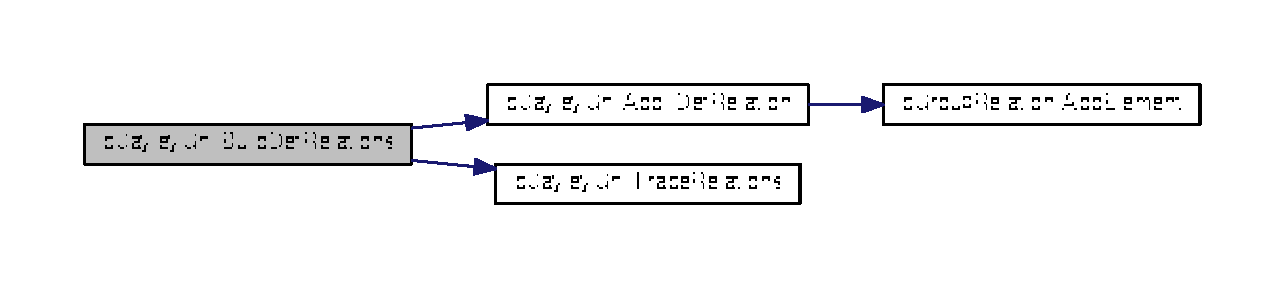
\includegraphics[width=350pt]{classcCayleyGrf_a8517436f6101a294fa7f30355efaa196_cgraph}
\end{center}
\end{figure}


\hypertarget{classcCayleyGrf_a4a0ff02aa7bb9d556456b34e9f66f3d9}{\index{c\-Cayley\-Grf@{c\-Cayley\-Grf}!\-Build\-Graph@{\-Build\-Graph}}
\index{\-Build\-Graph@{\-Build\-Graph}!cCayleyGrf@{c\-Cayley\-Grf}}
\subsubsection[{\-Build\-Graph}]{\setlength{\rightskip}{0pt plus 5cm}template$<$typename G $>$ void {\bf c\-Cayley\-Grf}$<$ \-G $>$\-::{\bf \-Build\-Graph} (
\begin{DoxyParamCaption}
{}
\end{DoxyParamCaption}
)\hspace{0.3cm}{\ttfamily  \mbox{[}inline\mbox{]}}}}\label{classcCayleyGrf_a4a0ff02aa7bb9d556456b34e9f66f3d9}
builds the \-Cayle graph as and adjacency list\-: the nodes are the indexes of the elements, the edges are the indexes of the generators \-Complexity\-: \-O(n$\ast$m), where n is the number of generators and m the number of elements \hypertarget{classcCayleyGrf_aeb4d8533b65921ca63fdaaf4516f92f6}{\index{c\-Cayley\-Grf@{c\-Cayley\-Grf}!\-Get\-Graph@{\-Get\-Graph}}
\index{\-Get\-Graph@{\-Get\-Graph}!cCayleyGrf@{c\-Cayley\-Grf}}
\subsubsection[{\-Get\-Graph}]{\setlength{\rightskip}{0pt plus 5cm}template$<$typename G $>$ \-Graph$\ast$ {\bf c\-Cayley\-Grf}$<$ \-G $>$\-::{\bf \-Get\-Graph} (
\begin{DoxyParamCaption}
{}
\end{DoxyParamCaption}
) const\hspace{0.3cm}{\ttfamily  \mbox{[}inline\mbox{]}}}}\label{classcCayleyGrf_aeb4d8533b65921ca63fdaaf4516f92f6}
returns the underlying graph representation (adjacency list) 

\-The documentation for this class was generated from the following file\-:\begin{DoxyCompactItemize}
\item 
cayley\-\_\-graph.\-h\end{DoxyCompactItemize}

\hypertarget{classcCayleyGrf_1_1cColourEdgesVis}{\section{c\-Cayley\-Grf$<$ \-G $>$\-:\-:c\-Colour\-Edges\-Vis$<$ \-E, \-Grf $>$ \-Class \-Template \-Reference}
\label{classcCayleyGrf_1_1cColourEdgesVis}\index{c\-Cayley\-Grf$<$ G $>$\-::c\-Colour\-Edges\-Vis$<$ E, Grf $>$@{c\-Cayley\-Grf$<$ G $>$\-::c\-Colour\-Edges\-Vis$<$ E, Grf $>$}}
}


\-Collaboration diagram for c\-Cayley\-Grf$<$ \-G $>$\-:\-:c\-Colour\-Edges\-Vis$<$ \-E, \-Grf $>$\-:
\nopagebreak
\begin{figure}[H]
\begin{center}
\leavevmode
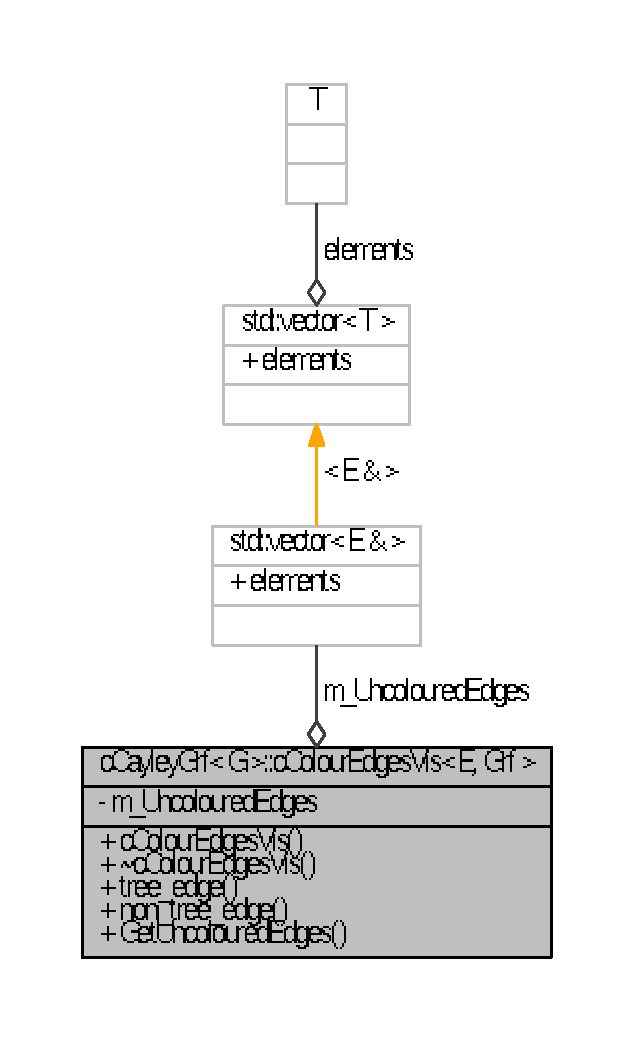
\includegraphics[width=310pt]{classcCayleyGrf_1_1cColourEdgesVis__coll__graph}
\end{center}
\end{figure}
\subsection*{\-Public \-Member \-Functions}
\begin{DoxyCompactItemize}
\item 
\hypertarget{classcCayleyGrf_1_1cColourEdgesVis_a6943930a8499e2dc40c1ff8d389e6aa2}{void {\bfseries tree\-\_\-edge} (\-E edge, const \-Grf \&graph)}\label{classcCayleyGrf_1_1cColourEdgesVis_a6943930a8499e2dc40c1ff8d389e6aa2}

\item 
\hypertarget{classcCayleyGrf_1_1cColourEdgesVis_a5e3642d81e1ae3e9bab5b063a9be440f}{void {\bfseries non\-\_\-tree\-\_\-edge} (\-E edge, const \-Grf \&graph)}\label{classcCayleyGrf_1_1cColourEdgesVis_a5e3642d81e1ae3e9bab5b063a9be440f}

\item 
std\-::vector$<$ \-E \& $>$ \& \hyperlink{classcCayleyGrf_1_1cColourEdgesVis_ab276cf1b92f16ca1aae832f0a1fdfdd9}{\-Get\-Uncoloured\-Edges} ()
\end{DoxyCompactItemize}
\subsection*{\-Private \-Attributes}
\begin{DoxyCompactItemize}
\item 
\hypertarget{classcCayleyGrf_1_1cColourEdgesVis_a5e243d1ea84763acd82dabb0faeadc62}{std\-::vector$<$ \-E \& $>$ {\bfseries m\-\_\-\-Uncoloured\-Edges}}\label{classcCayleyGrf_1_1cColourEdgesVis_a5e243d1ea84763acd82dabb0faeadc62}

\end{DoxyCompactItemize}
\subsubsection*{template$<$typename G$>$template$<$typename \-E, typename \-Grf$>$ class c\-Cayley\-Grf$<$ G $>$\-::c\-Colour\-Edges\-Vis$<$ E, Grf $>$}



\subsection{\-Member \-Function \-Documentation}
\hypertarget{classcCayleyGrf_1_1cColourEdgesVis_ab276cf1b92f16ca1aae832f0a1fdfdd9}{\index{c\-Cayley\-Grf\-::c\-Colour\-Edges\-Vis@{c\-Cayley\-Grf\-::c\-Colour\-Edges\-Vis}!\-Get\-Uncoloured\-Edges@{\-Get\-Uncoloured\-Edges}}
\index{\-Get\-Uncoloured\-Edges@{\-Get\-Uncoloured\-Edges}!cCayleyGrf::cColourEdgesVis@{c\-Cayley\-Grf\-::c\-Colour\-Edges\-Vis}}
\subsubsection[{\-Get\-Uncoloured\-Edges}]{\setlength{\rightskip}{0pt plus 5cm}template$<$typename G $>$ template$<$typename \-E, typename \-Grf$>$ std\-::vector$<$\-E\&$>$\& {\bf c\-Cayley\-Grf}$<$ \-G $>$\-::{\bf c\-Colour\-Edges\-Vis}$<$ \-E, \-Grf $>$\-::{\bf \-Get\-Uncoloured\-Edges} (
\begin{DoxyParamCaption}
{}
\end{DoxyParamCaption}
)\hspace{0.3cm}{\ttfamily  \mbox{[}inline\mbox{]}}}}\label{classcCayleyGrf_1_1cColourEdgesVis_ab276cf1b92f16ca1aae832f0a1fdfdd9}
returns the edges that are not contained in the spanning tree (that are not coloured) 

\-The documentation for this class was generated from the following file\-:\begin{DoxyCompactItemize}
\item 
cayley\-\_\-graph.\-h\end{DoxyCompactItemize}

\hypertarget{classcGenRep}{\section{c\-Gen\-Rep$<$ T $>$ Class Template Reference}
\label{classcGenRep}\index{c\-Gen\-Rep$<$ T $>$@{c\-Gen\-Rep$<$ T $>$}}
}


Collaboration diagram for c\-Gen\-Rep$<$ T $>$\-:
\subsection*{Public Member Functions}
\begin{DoxyCompactItemize}
\item 
\hypertarget{classcGenRep_afc45eb5aac4afa26288e4ef1b6dc3c52}{{\bfseries c\-Gen\-Rep} (tr1\-::unordered\-\_\-set$<$ T $>$ \&set)}\label{classcGenRep_afc45eb5aac4afa26288e4ef1b6dc3c52}

\item 
\hypertarget{classcGenRep_afb8d7535bcd9e4fda83eceb2a2633c2c}{tr1\-::unordered\-\_\-set$<$ T $>$\\*
\-::const\-\_\-iterator {\bfseries Get\-Random\-Iterator} () const }\label{classcGenRep_afb8d7535bcd9e4fda83eceb2a2633c2c}

\item 
\hypertarget{classcGenRep_aa94ce954bd3a2aabaa54d46642141df9}{tr1\-::unordered\-\_\-set$<$ T $>$ \& {\bfseries Get\-Group\-Set} () const }\label{classcGenRep_aa94ce954bd3a2aabaa54d46642141df9}

\item 
\hypertarget{classcGenRep_a38819c49300c51669a631399302ea130}{void {\bfseries Set\-Group\-Set} (tr1\-::unordered\-\_\-set$<$ T $>$ \&set)}\label{classcGenRep_a38819c49300c51669a631399302ea130}

\end{DoxyCompactItemize}
\subsection*{Public Attributes}
\begin{DoxyCompactItemize}
\item 
\hypertarget{classcGenRep_a94b066c9b99401b112085195c278b827}{tr1\-::unordered\-\_\-set$<$ T $>$\-::iterator {\bfseries Iterator\-Type}}\label{classcGenRep_a94b066c9b99401b112085195c278b827}

\end{DoxyCompactItemize}
\subsection*{Private Attributes}
\begin{DoxyCompactItemize}
\item 
\hypertarget{classcGenRep_af17e2ed953897003c229919293f6ecad}{tr1\-::unordered\-\_\-set$<$ T $>$ {\bfseries m\-\_\-\-Set}}\label{classcGenRep_af17e2ed953897003c229919293f6ecad}

\item 
\hypertarget{classcGenRep_aa7a645384a9a6036b4d860404557b88f}{std\-::size\-\_\-t {\bfseries m\-\_\-\-Group\-Order}}\label{classcGenRep_aa7a645384a9a6036b4d860404557b88f}

\end{DoxyCompactItemize}


The documentation for this class was generated from the following file\-:\begin{DoxyCompactItemize}
\item 
gen\-\_\-rep.\-h\end{DoxyCompactItemize}

\hypertarget{classcGroup}{\section{c\-Group$<$ \-T, group\-\_\-rep $>$ \-Class \-Template \-Reference}
\label{classcGroup}\index{c\-Group$<$ T, group\-\_\-rep $>$@{c\-Group$<$ T, group\-\_\-rep $>$}}
}


{\ttfamily \#include $<$group.\-h$>$}

\subsection*{\-Public \-Types}
\begin{DoxyCompactItemize}
\item 
\hypertarget{classcGroup_abf5ed8f308bc05dbbb75b1f2ccb3bf18}{typedef \-T {\bfseries \-Element\-Type}}\label{classcGroup_abf5ed8f308bc05dbbb75b1f2ccb3bf18}

\item 
\hypertarget{classcGroup_a8c16d6d9eb0d68d286505528c1e94d3a}{typedef \hyperlink{classcGroup}{c\-Group}$<$ \-T, group\-\_\-rep $>$ {\bfseries \-Self\-Type}}\label{classcGroup_a8c16d6d9eb0d68d286505528c1e94d3a}

\item 
\hypertarget{classcGroup_a8752843a8e5c6d23411de90d4e1a1f51}{typedef group\-\_\-rep$<$ \-T $>$ {\bfseries \-Rep\-Type}}\label{classcGroup_a8752843a8e5c6d23411de90d4e1a1f51}

\item 
\hypertarget{classcGroup_aa233178cfb06c6c59df798ff40fce156}{typedef std\-::vector$<$ \-Element\-Type $>$ {\bfseries \-Grp\-Vec}}\label{classcGroup_aa233178cfb06c6c59df798ff40fce156}

\end{DoxyCompactItemize}
\subsection*{\-Public \-Member \-Functions}
\begin{DoxyCompactItemize}
\item 
\hypertarget{classcGroup_a28f87c232c9d07ba9f9b0ec159e8243a}{{\bfseries c\-Group} (std\-::vector$<$ \-Element\-Type $>$ \&gr\-\_\-vec)}\label{classcGroup_a28f87c232c9d07ba9f9b0ec159e8243a}

\item 
\hypertarget{classcGroup_a38b515a0db10fa1fcebe7b635fc0d481}{{\bfseries c\-Group} (std\-::initializer\-\_\-list$<$ \-T $>$ ini\-\_\-list)}\label{classcGroup_a38b515a0db10fa1fcebe7b635fc0d481}

\item 
bool \hyperlink{classcGroup_acb69bf5f56805920d414a80ac5e54f36}{is\-Soluble} () const 
\item 
\hyperlink{classcSubgroup}{c\-Subgroup}$<$ \hyperlink{classcGroup}{\-Self\-Type} $>$ \hyperlink{classcGroup_a5177b0cd3b5a1c6d1dc7673c28fa14f0}{\-Get\-Centralizer} (const \hyperlink{classcSubgroup}{c\-Subgroup}$<$ \hyperlink{classcGroup}{\-Self\-Type} $>$ \&\-\_\-subgrp, \-Grp\-Vec \&grp\-\_\-el) const 
\item 
\hyperlink{classcSubgroup}{c\-Subgroup}$<$ \hyperlink{classcGroup}{\-Self\-Type} $>$ \hyperlink{classcGroup_ade523d25a78970fffa70f17d68643d15}{\-Get\-Center} (\-Grp\-Vec \&grp\-\_\-el) const 
\item 
\hyperlink{classcSubgroup}{c\-Subgroup}$<$ \hyperlink{classcGroup}{\-Self\-Type} $>$ \hyperlink{classcGroup_a1bcc2cdb6db5251b23cd099b25ffa057}{\-Get\-Normalizer} (const \hyperlink{classcSubgroup}{c\-Subgroup}$<$ \hyperlink{classcGroup}{\-Self\-Type} $>$ \&\-\_\-subgrp) const 
\item 
std\-::vector$<$ \-Element\-Type $>$ \hyperlink{classcGroup_ac0b8279834b59139afeb562be03937de}{\-Get\-Centralizer\-El} (\-Element\-Type \&element, \-Grp\-Vec \&grp\-\_\-el) const 
\item 
std\-::vector$<$ \-Element\-Type $>$ \hyperlink{classcGroup_aa0946d645c3ae06c56dc16f13a9f7ef2}{\-Get\-Center\-El} (\-Grp\-Vec \&grp\-\_\-el) const 
\item 
std\-::vector$<$ \-Element\-Type $>$ \hyperlink{classcGroup_a442a90478046593d38f5d131eb22b9a9}{\-Get\-Normalizer\-El} (const \hyperlink{classcSubgroup}{c\-Subgroup}$<$ \hyperlink{classcGroup}{\-Self\-Type} $>$ \&\-\_\-subgrp) const 
\end{DoxyCompactItemize}


\subsection{\-Detailed \-Description}
\subsubsection*{template$<$typename T, template$<$ typename $>$ class group\-\_\-rep = c\-Gen\-Rep$>$class c\-Group$<$ T, group\-\_\-rep $>$}

this class represents a group given by a set of generators it uses an internal representation given by the group\-\_\-rep template parameter and the type element \-T 

\subsection{\-Member \-Function \-Documentation}
\hypertarget{classcGroup_ade523d25a78970fffa70f17d68643d15}{\index{c\-Group@{c\-Group}!\-Get\-Center@{\-Get\-Center}}
\index{\-Get\-Center@{\-Get\-Center}!cGroup@{c\-Group}}
\subsubsection[{\-Get\-Center}]{\setlength{\rightskip}{0pt plus 5cm}template$<$typename T , template$<$ typename $>$ class group\-\_\-rep = c\-Gen\-Rep$>$ {\bf c\-Subgroup}$<${\bf \-Self\-Type}$>$ {\bf c\-Group}$<$ \-T, group\-\_\-rep $>$\-::{\bf \-Get\-Center} (
\begin{DoxyParamCaption}
\item[{\-Grp\-Vec \&}]{grp\-\_\-el}
\end{DoxyParamCaption}
) const\hspace{0.3cm}{\ttfamily  \mbox{[}inline\mbox{]}}}}\label{classcGroup_ade523d25a78970fffa70f17d68643d15}
returns the center subgroup of the group \-Z(\-G), the elements that comute with all the elements of the group 

\-Here is the call graph for this function\-:
\nopagebreak
\begin{figure}[H]
\begin{center}
\leavevmode
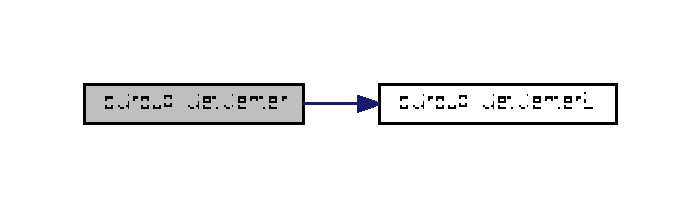
\includegraphics[width=340pt]{classcGroup_ade523d25a78970fffa70f17d68643d15_cgraph}
\end{center}
\end{figure}


\hypertarget{classcGroup_aa0946d645c3ae06c56dc16f13a9f7ef2}{\index{c\-Group@{c\-Group}!\-Get\-Center\-El@{\-Get\-Center\-El}}
\index{\-Get\-Center\-El@{\-Get\-Center\-El}!cGroup@{c\-Group}}
\subsubsection[{\-Get\-Center\-El}]{\setlength{\rightskip}{0pt plus 5cm}template$<$typename T , template$<$ typename $>$ class group\-\_\-rep = c\-Gen\-Rep$>$ std\-::vector$<$\-Element\-Type$>$ {\bf c\-Group}$<$ \-T, group\-\_\-rep $>$\-::{\bf \-Get\-Center\-El} (
\begin{DoxyParamCaption}
\item[{\-Grp\-Vec \&}]{grp\-\_\-el}
\end{DoxyParamCaption}
) const\hspace{0.3cm}{\ttfamily  \mbox{[}inline\mbox{]}}}}\label{classcGroup_aa0946d645c3ae06c56dc16f13a9f7ef2}
returns the centralizer subgroup of the group as a list of elements \hypertarget{classcGroup_a5177b0cd3b5a1c6d1dc7673c28fa14f0}{\index{c\-Group@{c\-Group}!\-Get\-Centralizer@{\-Get\-Centralizer}}
\index{\-Get\-Centralizer@{\-Get\-Centralizer}!cGroup@{c\-Group}}
\subsubsection[{\-Get\-Centralizer}]{\setlength{\rightskip}{0pt plus 5cm}template$<$typename T , template$<$ typename $>$ class group\-\_\-rep = c\-Gen\-Rep$>$ {\bf c\-Subgroup}$<${\bf \-Self\-Type}$>$ {\bf c\-Group}$<$ \-T, group\-\_\-rep $>$\-::{\bf \-Get\-Centralizer} (
\begin{DoxyParamCaption}
\item[{const {\bf c\-Subgroup}$<$ {\bf \-Self\-Type} $>$ \&}]{\-\_\-subgrp, }
\item[{\-Grp\-Vec \&}]{grp\-\_\-el}
\end{DoxyParamCaption}
) const\hspace{0.3cm}{\ttfamily  \mbox{[}inline\mbox{]}}}}\label{classcGroup_a5177b0cd3b5a1c6d1dc7673c28fa14f0}
returns the centralizer subgroup of the group using the given subgroup 

\-Here is the call graph for this function\-:
\nopagebreak
\begin{figure}[H]
\begin{center}
\leavevmode
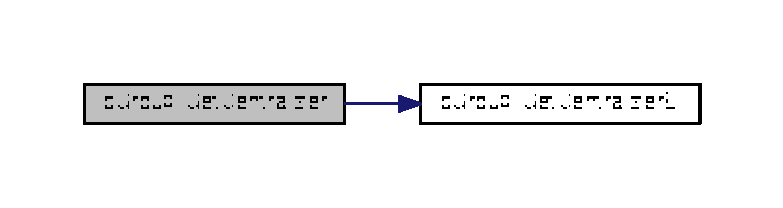
\includegraphics[width=350pt]{classcGroup_a5177b0cd3b5a1c6d1dc7673c28fa14f0_cgraph}
\end{center}
\end{figure}


\hypertarget{classcGroup_ac0b8279834b59139afeb562be03937de}{\index{c\-Group@{c\-Group}!\-Get\-Centralizer\-El@{\-Get\-Centralizer\-El}}
\index{\-Get\-Centralizer\-El@{\-Get\-Centralizer\-El}!cGroup@{c\-Group}}
\subsubsection[{\-Get\-Centralizer\-El}]{\setlength{\rightskip}{0pt plus 5cm}template$<$typename T , template$<$ typename $>$ class group\-\_\-rep = c\-Gen\-Rep$>$ std\-::vector$<$\-Element\-Type$>$ {\bf c\-Group}$<$ \-T, group\-\_\-rep $>$\-::{\bf \-Get\-Centralizer\-El} (
\begin{DoxyParamCaption}
\item[{\-Element\-Type \&}]{element, }
\item[{\-Grp\-Vec \&}]{grp\-\_\-el}
\end{DoxyParamCaption}
) const\hspace{0.3cm}{\ttfamily  \mbox{[}inline\mbox{]}}}}\label{classcGroup_ac0b8279834b59139afeb562be03937de}
returns the centralizer subgroup of a given element \hypertarget{classcGroup_a1bcc2cdb6db5251b23cd099b25ffa057}{\index{c\-Group@{c\-Group}!\-Get\-Normalizer@{\-Get\-Normalizer}}
\index{\-Get\-Normalizer@{\-Get\-Normalizer}!cGroup@{c\-Group}}
\subsubsection[{\-Get\-Normalizer}]{\setlength{\rightskip}{0pt plus 5cm}template$<$typename T , template$<$ typename $>$ class group\-\_\-rep = c\-Gen\-Rep$>$ {\bf c\-Subgroup}$<${\bf \-Self\-Type}$>$ {\bf c\-Group}$<$ \-T, group\-\_\-rep $>$\-::{\bf \-Get\-Normalizer} (
\begin{DoxyParamCaption}
\item[{const {\bf c\-Subgroup}$<$ {\bf \-Self\-Type} $>$ \&}]{\-\_\-subgrp}
\end{DoxyParamCaption}
) const\hspace{0.3cm}{\ttfamily  \mbox{[}inline\mbox{]}}}}\label{classcGroup_a1bcc2cdb6db5251b23cd099b25ffa057}
returns the normalizer subgroup, given a subgroup 

\-Here is the call graph for this function\-:
\nopagebreak
\begin{figure}[H]
\begin{center}
\leavevmode
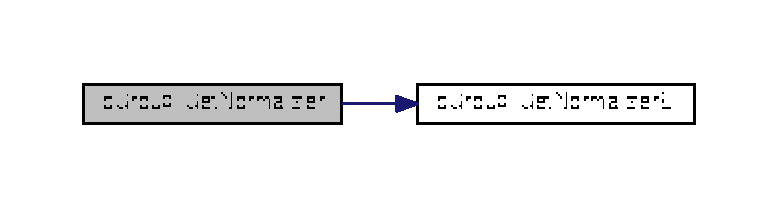
\includegraphics[width=350pt]{classcGroup_a1bcc2cdb6db5251b23cd099b25ffa057_cgraph}
\end{center}
\end{figure}


\hypertarget{classcGroup_a442a90478046593d38f5d131eb22b9a9}{\index{c\-Group@{c\-Group}!\-Get\-Normalizer\-El@{\-Get\-Normalizer\-El}}
\index{\-Get\-Normalizer\-El@{\-Get\-Normalizer\-El}!cGroup@{c\-Group}}
\subsubsection[{\-Get\-Normalizer\-El}]{\setlength{\rightskip}{0pt plus 5cm}template$<$typename T , template$<$ typename $>$ class group\-\_\-rep = c\-Gen\-Rep$>$ std\-::vector$<$\-Element\-Type$>$ {\bf c\-Group}$<$ \-T, group\-\_\-rep $>$\-::{\bf \-Get\-Normalizer\-El} (
\begin{DoxyParamCaption}
\item[{const {\bf c\-Subgroup}$<$ {\bf \-Self\-Type} $>$ \&}]{\-\_\-subgrp}
\end{DoxyParamCaption}
) const\hspace{0.3cm}{\ttfamily  \mbox{[}inline\mbox{]}}}}\label{classcGroup_a442a90478046593d38f5d131eb22b9a9}
\-T\-O\-D\-O -\/-\/ check for bugs returns the normalizer subgroup of the given subgroup as a list of elements \hypertarget{classcGroup_acb69bf5f56805920d414a80ac5e54f36}{\index{c\-Group@{c\-Group}!is\-Soluble@{is\-Soluble}}
\index{is\-Soluble@{is\-Soluble}!cGroup@{c\-Group}}
\subsubsection[{is\-Soluble}]{\setlength{\rightskip}{0pt plus 5cm}template$<$typename T , template$<$ typename $>$ class group\-\_\-rep = c\-Gen\-Rep$>$ bool {\bf c\-Group}$<$ \-T, group\-\_\-rep $>$\-::{\bf is\-Soluble} (
\begin{DoxyParamCaption}
{}
\end{DoxyParamCaption}
) const\hspace{0.3cm}{\ttfamily  \mbox{[}inline\mbox{]}}}}\label{classcGroup_acb69bf5f56805920d414a80ac5e54f36}
\-T\-O\-D\-O implement this ? returns true if the group is soluble 

\-The documentation for this class was generated from the following file\-:\begin{DoxyCompactItemize}
\item 
group.\-h\end{DoxyCompactItemize}

\hypertarget{classcGroupElem}{\section{c\-Group\-Elem$<$ \-T, \-Binary\-Op $>$ \-Class \-Template \-Reference}
\label{classcGroupElem}\index{c\-Group\-Elem$<$ T, Binary\-Op $>$@{c\-Group\-Elem$<$ T, Binary\-Op $>$}}
}


{\ttfamily \#include $<$group\-\_\-elem.\-h$>$}

\subsection*{\-Public \-Types}
\begin{DoxyCompactItemize}
\item 
\hypertarget{classcGroupElem_a59d8e25f570c976b3c7f13756ada8dc4}{typedef \hyperlink{classcGroupElem}{c\-Group\-Elem}$<$ \-T, \-Binary\-Op $>$ {\bfseries \-Self\-Type}}\label{classcGroupElem_a59d8e25f570c976b3c7f13756ada8dc4}

\item 
\hypertarget{classcGroupElem_a49af5748a3d451f2256fb82266338bca}{typedef \-T {\bfseries \-Concrete\-El\-Type}}\label{classcGroupElem_a49af5748a3d451f2256fb82266338bca}

\end{DoxyCompactItemize}
\subsection*{\-Public \-Member \-Functions}
\begin{DoxyCompactItemize}
\item 
\hypertarget{classcGroupElem_ac677380fd35b7307be8230e01c47d24a}{{\bfseries c\-Group\-Elem} (\-T \&concrete\-\_\-obj)}\label{classcGroupElem_ac677380fd35b7307be8230e01c47d24a}

\item 
\hypertarget{classcGroupElem_a7e61b42847fb382a00025af19baf2132}{{\bfseries c\-Group\-Elem} (const \-T \&concrete\-\_\-obj)}\label{classcGroupElem_a7e61b42847fb382a00025af19baf2132}

\item 
\hypertarget{classcGroupElem_a13a796803737218c08e3d6bb652732d1}{{\bfseries c\-Group\-Elem} (const std\-::initializer\-\_\-list$<$ std\-::size\-\_\-t $>$ \&perm\-\_\-sq)}\label{classcGroupElem_a13a796803737218c08e3d6bb652732d1}

\item 
\hypertarget{classcGroupElem_aaa558bbe798129dccc53712777e1bd4e}{{\bfseries c\-Group\-Elem} (std\-::size\-\_\-t size, const std\-::initializer\-\_\-list$<$ std\-::size\-\_\-t $>$ \&perm\-\_\-sq)}\label{classcGroupElem_aaa558bbe798129dccc53712777e1bd4e}

\item 
\hypertarget{classcGroupElem_af2fe12bf9a1291a5c30905449e2b3a2b}{{\bfseries c\-Group\-Elem} (const \hyperlink{classcGroupElem}{\-Self\-Type} \&group\-\_\-elem)}\label{classcGroupElem_af2fe12bf9a1291a5c30905449e2b3a2b}

\item 
\hypertarget{classcGroupElem_a75d7cd6508130c2632042fa42041b874}{\hyperlink{classcGroupElem}{\-Self\-Type} \& {\bfseries operator=} (const \hyperlink{classcGroupElem}{\-Self\-Type} \&elem)}\label{classcGroupElem_a75d7cd6508130c2632042fa42041b874}

\item 
std\-::size\-\_\-t \hyperlink{classcGroupElem_ac29fd7c4409752f596249999d87e64ca}{\-Get\-Order} () const 
\item 
std\-::size\-\_\-t \hyperlink{classcGroupElem_a6f563c99529cb747e414fc20a8915a20}{\-Get\-Order} (std\-::size\-\_\-t group\-\_\-order)
\item 
\hyperlink{classcGroupElem}{\-Self\-Type} \hyperlink{classcGroupElem_a17bf17389d7b17e8674ef33eabed9163}{\-Get\-Inverse} () const 
\item 
\hyperlink{classcGroupElem}{\-Self\-Type} \hyperlink{classcGroupElem_af58088ba8679e49a4b1a34b503a649e0}{\-Get\-Nth\-Power} (std\-::size\-\_\-t n) const 
\item 
bool \hyperlink{classcGroupElem_ab0e3d62bb8a37b59a371188f320bdbca}{\-Commutes\-With} (const \hyperlink{classcGroupElem}{\-Self\-Type} \&element) const 
\item 
bool \hyperlink{classcGroupElem_ab01a807aff26daecd39cea6837b01e8e}{\-Is\-Normalizer} (const std\-::vector$<$ \hyperlink{classcGroupElem}{\-Self\-Type} $>$ \&elements) const 
\item 
\hyperlink{classcGroupElem}{\-Self\-Type} \hyperlink{classcGroupElem_ae394d9b317db051ae804ae299f173e3d}{\-Get\-Identity} () const 
\item 
\hypertarget{classcGroupElem_ab715bd9431a5b66e0230f9477339cecb}{\-Binary\-Op {\bfseries \-Get\-Binary\-Op} () const }\label{classcGroupElem_ab715bd9431a5b66e0230f9477339cecb}

\end{DoxyCompactItemize}
\subsection*{\-Private \-Member \-Functions}
\begin{DoxyCompactItemize}
\item 
\hyperlink{classcGroupElem}{\-Self\-Type} \hyperlink{classcGroupElem_a369cfffe505951aed65696857b25319b}{\-Get\-Nth\-Power} (std\-::size\-\_\-t n, const \hyperlink{classcGroupElem}{\-Self\-Type} \&element) const 
\end{DoxyCompactItemize}
\subsection*{\-Private \-Attributes}
\begin{DoxyCompactItemize}
\item 
\hypertarget{classcGroupElem_a9a6f51b4a5ce6a3b9dc8bff7a4812fec}{\-Binary\-Op {\bfseries m\-\_\-\-Bin\-Op}}\label{classcGroupElem_a9a6f51b4a5ce6a3b9dc8bff7a4812fec}

\end{DoxyCompactItemize}


\subsection{\-Detailed \-Description}
\subsubsection*{template$<$typename \-T, typename \-Binary\-Op$>$class c\-Group\-Elem$<$ T, Binary\-Op $>$}

generic class that represents a group element must be instatiated with the concrete element type and the binary operation(used as a policy) that is going to used with the element 

\subsection{\-Member \-Function \-Documentation}
\hypertarget{classcGroupElem_ab0e3d62bb8a37b59a371188f320bdbca}{\index{c\-Group\-Elem@{c\-Group\-Elem}!\-Commutes\-With@{\-Commutes\-With}}
\index{\-Commutes\-With@{\-Commutes\-With}!cGroupElem@{c\-Group\-Elem}}
\subsubsection[{\-Commutes\-With}]{\setlength{\rightskip}{0pt plus 5cm}template$<$typename \-T, typename \-Binary\-Op$>$ bool {\bf c\-Group\-Elem}$<$ \-T, \-Binary\-Op $>$\-::{\bf \-Commutes\-With} (
\begin{DoxyParamCaption}
\item[{const {\bf \-Self\-Type} \&}]{element}
\end{DoxyParamCaption}
) const\hspace{0.3cm}{\ttfamily  \mbox{[}inline\mbox{]}}}}\label{classcGroupElem_ab0e3d62bb8a37b59a371188f320bdbca}
return true if the element commutes with the element given as parameter \hypertarget{classcGroupElem_ae394d9b317db051ae804ae299f173e3d}{\index{c\-Group\-Elem@{c\-Group\-Elem}!\-Get\-Identity@{\-Get\-Identity}}
\index{\-Get\-Identity@{\-Get\-Identity}!cGroupElem@{c\-Group\-Elem}}
\subsubsection[{\-Get\-Identity}]{\setlength{\rightskip}{0pt plus 5cm}template$<$typename \-T, typename \-Binary\-Op$>$ {\bf \-Self\-Type} {\bf c\-Group\-Elem}$<$ \-T, \-Binary\-Op $>$\-::{\bf \-Get\-Identity} (
\begin{DoxyParamCaption}
{}
\end{DoxyParamCaption}
) const\hspace{0.3cm}{\ttfamily  \mbox{[}inline\mbox{]}}}}\label{classcGroupElem_ae394d9b317db051ae804ae299f173e3d}
returns the identity of the element type according to the binary operation \hypertarget{classcGroupElem_a17bf17389d7b17e8674ef33eabed9163}{\index{c\-Group\-Elem@{c\-Group\-Elem}!\-Get\-Inverse@{\-Get\-Inverse}}
\index{\-Get\-Inverse@{\-Get\-Inverse}!cGroupElem@{c\-Group\-Elem}}
\subsubsection[{\-Get\-Inverse}]{\setlength{\rightskip}{0pt plus 5cm}template$<$typename \-T, typename \-Binary\-Op$>$ {\bf \-Self\-Type} {\bf c\-Group\-Elem}$<$ \-T, \-Binary\-Op $>$\-::{\bf \-Get\-Inverse} (
\begin{DoxyParamCaption}
{}
\end{DoxyParamCaption}
) const\hspace{0.3cm}{\ttfamily  \mbox{[}inline\mbox{]}}}}\label{classcGroupElem_a17bf17389d7b17e8674ef33eabed9163}
returns the inverse of the element according to the given binaryu operation \hypertarget{classcGroupElem_af58088ba8679e49a4b1a34b503a649e0}{\index{c\-Group\-Elem@{c\-Group\-Elem}!\-Get\-Nth\-Power@{\-Get\-Nth\-Power}}
\index{\-Get\-Nth\-Power@{\-Get\-Nth\-Power}!cGroupElem@{c\-Group\-Elem}}
\subsubsection[{\-Get\-Nth\-Power}]{\setlength{\rightskip}{0pt plus 5cm}template$<$typename \-T, typename \-Binary\-Op$>$ {\bf \-Self\-Type} {\bf c\-Group\-Elem}$<$ \-T, \-Binary\-Op $>$\-::{\bf \-Get\-Nth\-Power} (
\begin{DoxyParamCaption}
\item[{std\-::size\-\_\-t}]{n}
\end{DoxyParamCaption}
) const\hspace{0.3cm}{\ttfamily  \mbox{[}inline\mbox{]}}}}\label{classcGroupElem_af58088ba8679e49a4b1a34b503a649e0}
returns the nth power of the element \hypertarget{classcGroupElem_a369cfffe505951aed65696857b25319b}{\index{c\-Group\-Elem@{c\-Group\-Elem}!\-Get\-Nth\-Power@{\-Get\-Nth\-Power}}
\index{\-Get\-Nth\-Power@{\-Get\-Nth\-Power}!cGroupElem@{c\-Group\-Elem}}
\subsubsection[{\-Get\-Nth\-Power}]{\setlength{\rightskip}{0pt plus 5cm}template$<$typename \-T, typename \-Binary\-Op$>$ {\bf \-Self\-Type} {\bf c\-Group\-Elem}$<$ \-T, \-Binary\-Op $>$\-::{\bf \-Get\-Nth\-Power} (
\begin{DoxyParamCaption}
\item[{std\-::size\-\_\-t}]{n, }
\item[{const {\bf \-Self\-Type} \&}]{element}
\end{DoxyParamCaption}
) const\hspace{0.3cm}{\ttfamily  \mbox{[}inline, private\mbox{]}}}}\label{classcGroupElem_a369cfffe505951aed65696857b25319b}
recursive function that actually computes the nth power \-Complexity\-: $ O(log_2(n)) $ 

\-Here is the call graph for this function\-:\nopagebreak
\begin{figure}[H]
\begin{center}
\leavevmode
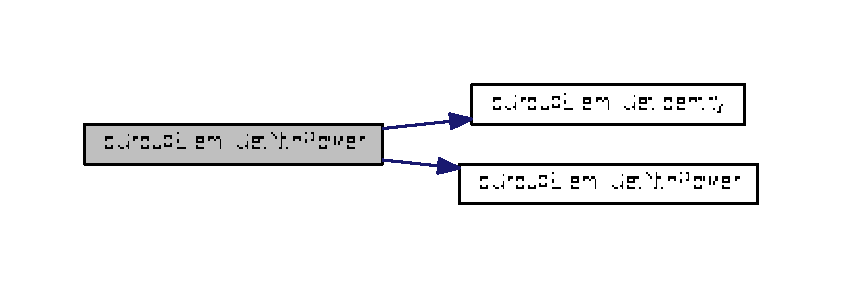
\includegraphics[width=350pt]{classcGroupElem_a369cfffe505951aed65696857b25319b_cgraph}
\end{center}
\end{figure}


\hypertarget{classcGroupElem_ac29fd7c4409752f596249999d87e64ca}{\index{c\-Group\-Elem@{c\-Group\-Elem}!\-Get\-Order@{\-Get\-Order}}
\index{\-Get\-Order@{\-Get\-Order}!cGroupElem@{c\-Group\-Elem}}
\subsubsection[{\-Get\-Order}]{\setlength{\rightskip}{0pt plus 5cm}template$<$typename \-T, typename \-Binary\-Op$>$ std\-::size\-\_\-t {\bf c\-Group\-Elem}$<$ \-T, \-Binary\-Op $>$\-::{\bf \-Get\-Order} (
\begin{DoxyParamCaption}
{}
\end{DoxyParamCaption}
) const\hspace{0.3cm}{\ttfamily  \mbox{[}inline\mbox{]}}}}\label{classcGroupElem_ac29fd7c4409752f596249999d87e64ca}
returns the identity element corresponding to the given element type and the binary operation \-Complexity\-: \-O(n) multiplications and comparisons, where n is the order 

\-Here is the call graph for this function\-:\nopagebreak
\begin{figure}[H]
\begin{center}
\leavevmode
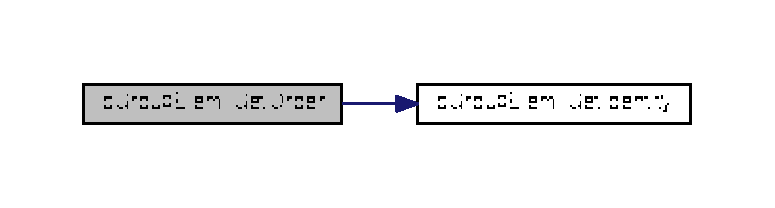
\includegraphics[width=350pt]{classcGroupElem_ac29fd7c4409752f596249999d87e64ca_cgraph}
\end{center}
\end{figure}


\hypertarget{classcGroupElem_a6f563c99529cb747e414fc20a8915a20}{\index{c\-Group\-Elem@{c\-Group\-Elem}!\-Get\-Order@{\-Get\-Order}}
\index{\-Get\-Order@{\-Get\-Order}!cGroupElem@{c\-Group\-Elem}}
\subsubsection[{\-Get\-Order}]{\setlength{\rightskip}{0pt plus 5cm}template$<$typename \-T, typename \-Binary\-Op$>$ std\-::size\-\_\-t {\bf c\-Group\-Elem}$<$ \-T, \-Binary\-Op $>$\-::{\bf \-Get\-Order} (
\begin{DoxyParamCaption}
\item[{std\-::size\-\_\-t}]{group\-\_\-order}
\end{DoxyParamCaption}
)\hspace{0.3cm}{\ttfamily  \mbox{[}inline\mbox{]}}}}\label{classcGroupElem_a6f563c99529cb747e414fc20a8915a20}
returns the identity element corresponding to the given element type and the binary operation using the given group order \-Complexity\-: \-O(n) multiplication and d comparisons, where n is the order, and d is the number of divisors of the order of the group 

\-Here is the call graph for this function\-:\nopagebreak
\begin{figure}[H]
\begin{center}
\leavevmode
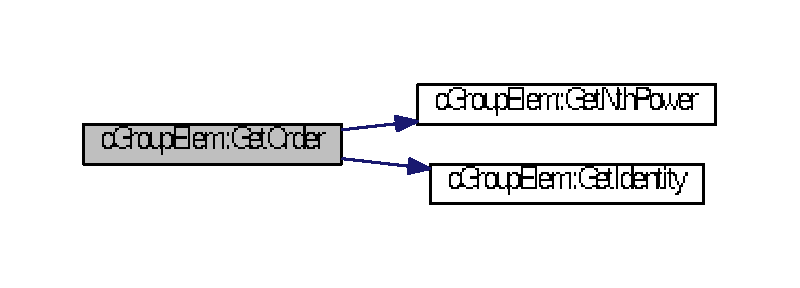
\includegraphics[width=350pt]{classcGroupElem_a6f563c99529cb747e414fc20a8915a20_cgraph}
\end{center}
\end{figure}


\hypertarget{classcGroupElem_ab01a807aff26daecd39cea6837b01e8e}{\index{c\-Group\-Elem@{c\-Group\-Elem}!\-Is\-Normalizer@{\-Is\-Normalizer}}
\index{\-Is\-Normalizer@{\-Is\-Normalizer}!cGroupElem@{c\-Group\-Elem}}
\subsubsection[{\-Is\-Normalizer}]{\setlength{\rightskip}{0pt plus 5cm}template$<$typename \-T, typename \-Binary\-Op$>$ bool {\bf c\-Group\-Elem}$<$ \-T, \-Binary\-Op $>$\-::{\bf \-Is\-Normalizer} (
\begin{DoxyParamCaption}
\item[{const std\-::vector$<$ {\bf \-Self\-Type} $>$ \&}]{elements}
\end{DoxyParamCaption}
) const\hspace{0.3cm}{\ttfamily  \mbox{[}inline\mbox{]}}}}\label{classcGroupElem_ab01a807aff26daecd39cea6837b01e8e}
returns true if the element is a normalizer for the list of elements given as parameter 

\-Here is the call graph for this function\-:\nopagebreak
\begin{figure}[H]
\begin{center}
\leavevmode
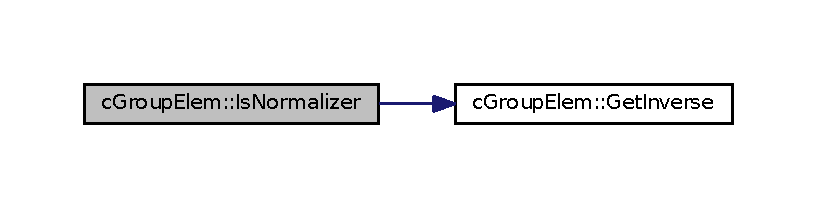
\includegraphics[width=350pt]{classcGroupElem_ab01a807aff26daecd39cea6837b01e8e_cgraph}
\end{center}
\end{figure}




\-The documentation for this class was generated from the following file\-:\begin{DoxyCompactItemize}
\item 
group\-\_\-elem.\-h\end{DoxyCompactItemize}

\hypertarget{classcGroupRelation}{\section{c\-Group\-Relation$<$ \-T $>$ \-Class \-Template \-Reference}
\label{classcGroupRelation}\index{c\-Group\-Relation$<$ T $>$@{c\-Group\-Relation$<$ T $>$}}
}


\-Inheritance diagram for c\-Group\-Relation$<$ \-T $>$\-:\nopagebreak
\begin{figure}[H]
\begin{center}
\leavevmode
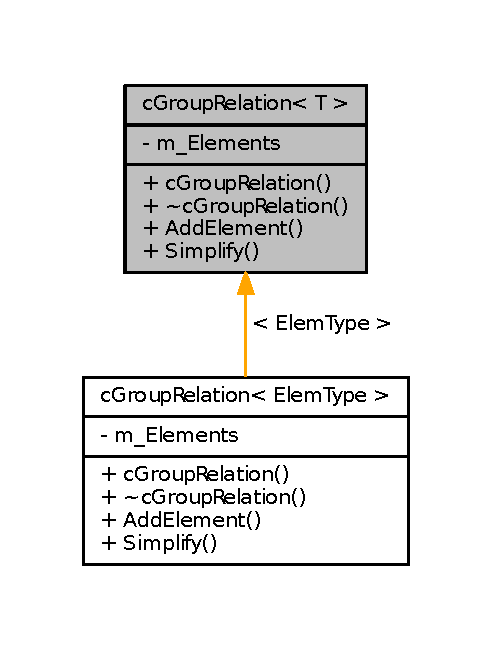
\includegraphics[width=234pt]{classcGroupRelation__inherit__graph}
\end{center}
\end{figure}


\-Collaboration diagram for c\-Group\-Relation$<$ \-T $>$\-:\nopagebreak
\begin{figure}[H]
\begin{center}
\leavevmode
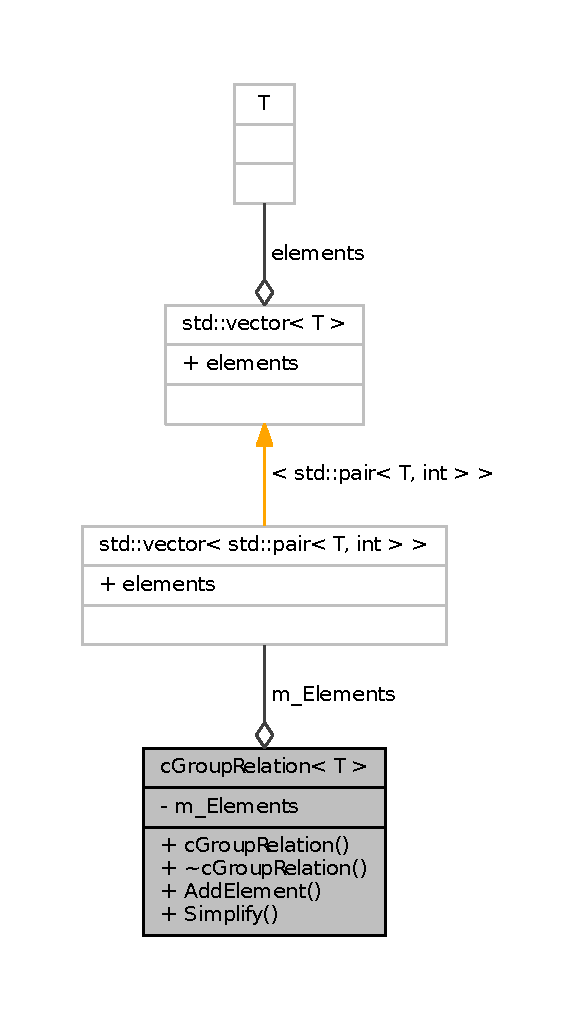
\includegraphics[width=260pt]{classcGroupRelation__coll__graph}
\end{center}
\end{figure}
\subsection*{\-Public \-Member \-Functions}
\begin{DoxyCompactItemize}
\item 
\hypertarget{classcGroupRelation_aeae9fe8f02b40a3cf1b7f73abee2b9cd}{void {\bfseries \-Add\-Element} (\-T \&element, int power)}\label{classcGroupRelation_aeae9fe8f02b40a3cf1b7f73abee2b9cd}

\item 
\hypertarget{classcGroupRelation_ac93e1c0794cbca8e574cbf1c4255c675}{void {\bfseries \-Simplify} ()}\label{classcGroupRelation_ac93e1c0794cbca8e574cbf1c4255c675}

\end{DoxyCompactItemize}
\subsection*{\-Private \-Attributes}
\begin{DoxyCompactItemize}
\item 
\hypertarget{classcGroupRelation_a71fe79690808fb895d27eee80edc99d4}{std\-::vector$<$ std\-::pair$<$ \-T, int $>$ $>$ {\bfseries m\-\_\-\-Elements}}\label{classcGroupRelation_a71fe79690808fb895d27eee80edc99d4}

\end{DoxyCompactItemize}
\subsubsection*{template$<$typename \-T$>$ class c\-Group\-Relation$<$ T $>$}



\-The documentation for this class was generated from the following file\-:\begin{DoxyCompactItemize}
\item 
group\-\_\-relation.\-h\end{DoxyCompactItemize}

\hypertarget{classcGrpLattice}{\section{c\-Grp\-Lattice$<$ \-G $>$ \-Class \-Template \-Reference}
\label{classcGrpLattice}\index{c\-Grp\-Lattice$<$ G $>$@{c\-Grp\-Lattice$<$ G $>$}}
}


{\ttfamily \#include $<$group\-\_\-lattice.\-h$>$}



\-Collaboration diagram for c\-Grp\-Lattice$<$ \-G $>$\-:\nopagebreak
\begin{figure}[H]
\begin{center}
\leavevmode
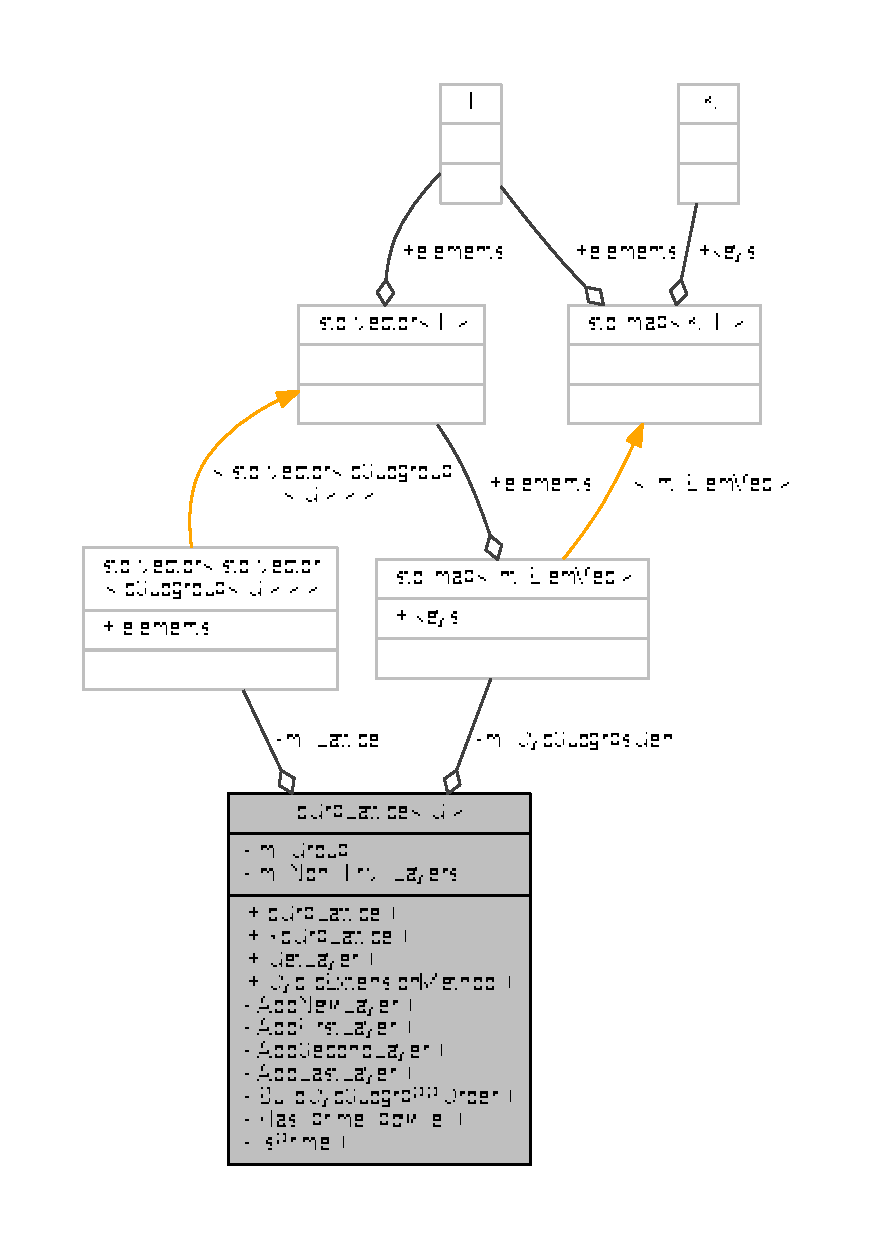
\includegraphics[width=350pt]{classcGrpLattice__coll__graph}
\end{center}
\end{figure}
\subsection*{\-Public \-Types}
\begin{DoxyCompactItemize}
\item 
\hypertarget{classcGrpLattice_adcd74a778419c1f515170d6f4eec0e46}{typedef \-G\-::\-Element\-Type {\bfseries \-T}}\label{classcGrpLattice_adcd74a778419c1f515170d6f4eec0e46}

\item 
\hypertarget{classcGrpLattice_a65bbb53481fb01fab29b56111e08a1a8}{typedef std\-::vector$<$ \hyperlink{classcSubgroup}{c\-Subgroup}\*
$<$ \-G $>$ $>$\-::iterator {\bfseries \-Sub\-Grp\-\_\-\-Iterator}}\label{classcGrpLattice_a65bbb53481fb01fab29b56111e08a1a8}

\item 
\hypertarget{classcGrpLattice_a229b8231e9d4977673fcc629c083ed27}{typedef \hyperlink{classcGrpLattice}{c\-Grp\-Lattice}$<$ \-G $>$ {\bfseries \-Self\-Type}}\label{classcGrpLattice_a229b8231e9d4977673fcc629c083ed27}

\item 
\hypertarget{classcGrpLattice_ae5a1bef06325a01169039dfbbfcd279a}{typedef std\-::vector$<$ \-T $>$ {\bfseries \-Elem\-Vec}}\label{classcGrpLattice_ae5a1bef06325a01169039dfbbfcd279a}

\end{DoxyCompactItemize}
\subsection*{\-Public \-Member \-Functions}
\begin{DoxyCompactItemize}
\item 
\hypertarget{classcGrpLattice_a27f923e1817bed7d7d3b51a02d08bf76}{{\bfseries c\-Grp\-Lattice} (\-G \&group)}\label{classcGrpLattice_a27f923e1817bed7d7d3b51a02d08bf76}

\item 
\hypertarget{classcGrpLattice_a37b06de9e9bf5b647c524f000b054b6a}{std\-::vector$<$ \hyperlink{classcSubgroup}{c\-Subgroup}$<$ \-G $>$ $>$ \& {\bfseries \-Get\-Layer} (const std\-::size\-\_\-t index)}\label{classcGrpLattice_a37b06de9e9bf5b647c524f000b054b6a}

\item 
\hypertarget{classcGrpLattice_af05dbd664f73f60ea2e9bcef893da25b}{void {\bfseries \-Cyclic\-Extension\-Method} ()}\label{classcGrpLattice_af05dbd664f73f60ea2e9bcef893da25b}

\end{DoxyCompactItemize}
\subsection*{\-Private \-Member \-Functions}
\begin{DoxyCompactItemize}
\item 
\hypertarget{classcGrpLattice_a97f11569f3baaaff7c69510862ed3fed}{void {\bfseries \-Add\-New\-Layer} ()}\label{classcGrpLattice_a97f11569f3baaaff7c69510862ed3fed}

\item 
\hypertarget{classcGrpLattice_a0329e3be94f1e33f1da948d8cd9f2fae}{void {\bfseries \-Add\-First\-Layer} ()}\label{classcGrpLattice_a0329e3be94f1e33f1da948d8cd9f2fae}

\item 
\hypertarget{classcGrpLattice_a7219462f7ddb6eccf4220284c6b1dd3d}{void {\bfseries \-Add\-Second\-Layer} ()}\label{classcGrpLattice_a7219462f7ddb6eccf4220284c6b1dd3d}

\item 
\hypertarget{classcGrpLattice_a9060d3fa6007580cb76588d3a4ad6608}{void {\bfseries \-Add\-Last\-Layer} ()}\label{classcGrpLattice_a9060d3fa6007580cb76588d3a4ad6608}

\item 
\hypertarget{classcGrpLattice_a1fc6e598f0078312848813d97dac5764}{void {\bfseries \-Build\-Cyc\-Subgrp\-P\-P\-Order} ()}\label{classcGrpLattice_a1fc6e598f0078312848813d97dac5764}

\item 
\hypertarget{classcGrpLattice_a503aa173993abf544e0ccc1fe56e929d}{bool {\bfseries \-Has\-\_\-prime\-\_\-pow\-\_\-el} (const \hyperlink{classcSubgroup}{c\-Subgroup}$<$ \-G $>$ grp, const \-T element) const }\label{classcGrpLattice_a503aa173993abf544e0ccc1fe56e929d}

\item 
\hypertarget{classcGrpLattice_a496a3bf31e7cd52b5985ec916c10131e}{bool {\bfseries is\-Prime} (int number)}\label{classcGrpLattice_a496a3bf31e7cd52b5985ec916c10131e}

\end{DoxyCompactItemize}
\subsection*{\-Private \-Attributes}
\begin{DoxyCompactItemize}
\item 
\hypertarget{classcGrpLattice_adf219732413e288dd67173189a556bba}{\-G {\bfseries m\-\_\-\-Group}}\label{classcGrpLattice_adf219732413e288dd67173189a556bba}

\item 
\hypertarget{classcGrpLattice_a016e9d166b7cd74ef416bb4c4a22dfcc}{std\-::map$<$ int, \-Elem\-Vec $>$ {\bfseries m\-\_\-\-Cyc\-Subgrps\-Gen}}\label{classcGrpLattice_a016e9d166b7cd74ef416bb4c4a22dfcc}

\item 
\hypertarget{classcGrpLattice_a8a7ab9311e816bfa58c1f8ba727c5033}{std\-::vector$<$ std\-::vector\*
$<$ \hyperlink{classcSubgroup}{c\-Subgroup}$<$ \-G $>$ $>$ $>$ {\bfseries m\-\_\-\-Lattice}}\label{classcGrpLattice_a8a7ab9311e816bfa58c1f8ba727c5033}

\item 
\hypertarget{classcGrpLattice_a2060764d98fd699bc63323b1d5eafb63}{std\-::size\-\_\-t {\bfseries m\-\_\-\-Non\-\_\-\-Triv\-\_\-\-Layers}}\label{classcGrpLattice_a2060764d98fd699bc63323b1d5eafb63}

\end{DoxyCompactItemize}
\subsection*{\-Friends}
\begin{DoxyCompactItemize}
\item 
\hypertarget{classcGrpLattice_a96ca24361f58299e265ac93d1296733b}{std\-::ostream \& {\bfseries operator$<$$<$} (std\-::ostream \&out, \hyperlink{classcGrpLattice}{\-Self\-Type} \&lattice)}\label{classcGrpLattice_a96ca24361f58299e265ac93d1296733b}

\end{DoxyCompactItemize}


\subsection{\-Detailed \-Description}
\subsubsection*{template$<$typename G$>$class c\-Grp\-Lattice$<$ G $>$}

this class is under construction (not working yet) 

\-The documentation for this class was generated from the following file\-:\begin{DoxyCompactItemize}
\item 
group\-\_\-lattice.\-h\end{DoxyCompactItemize}

\hypertarget{classcHomomorphism}{
\section{c\-Homomorphism$<$ \-G1, \-G2 $>$ \-Class \-Template \-Reference}
\label{classcHomomorphism}\index{c\-Homomorphism$<$ G1, G2 $>$@{c\-Homomorphism$<$ G1, G2 $>$}}
}
\subsection*{\-Public \-Member \-Functions}
\begin{DoxyCompactItemize}
\item 
\hypertarget{classcHomomorphism_a826f07eaa6c431de9fc8ad236ebb7502}{
{\bfseries c\-Homomorphism} (\-G1 \&group, \-G2 \&group, \-Function\-Type map)}
\label{classcHomomorphism_a826f07eaa6c431de9fc8ad236ebb7502}

\item 
\hypertarget{classcHomomorphism_a4f6919efcd1c8446207a5150e3f29143}{
void {\bfseries \-Compute} ()}
\label{classcHomomorphism_a4f6919efcd1c8446207a5150e3f29143}

\item 
\hypertarget{classcHomomorphism_a0afe7b713cdb3e7628d049011334b539}{
void {\bfseries \-Display} ()}
\label{classcHomomorphism_a0afe7b713cdb3e7628d049011334b539}

\item 
\hypertarget{classcHomomorphism_a0f6fe4c7df91a345cd26023cf9b7c29d}{
\hyperlink{classcSubgroup}{c\-Subgroup}$<$ \-G1 $>$ {\bfseries \-Get\-Kernel} () const }
\label{classcHomomorphism_a0f6fe4c7df91a345cd26023cf9b7c29d}

\item 
\hypertarget{classcHomomorphism_ae2a5c5ab1fea57af03dbb926b05c5edc}{
\hyperlink{classcSubgroup}{c\-Subgroup}$<$ \-G2 $>$ {\bfseries \-Get\-Image} () const }
\label{classcHomomorphism_ae2a5c5ab1fea57af03dbb926b05c5edc}

\item 
\hypertarget{classcHomomorphism_ae5514786d9d5f0a185e5465c11075f13}{
\-B\-O\-O\-L {\bfseries is\-Isomorphism} () const }
\label{classcHomomorphism_ae5514786d9d5f0a185e5465c11075f13}

\end{DoxyCompactItemize}
\subsection*{\-Private \-Attributes}
\begin{DoxyCompactItemize}
\item 
\hypertarget{classcHomomorphism_a8b597c591cbbfb2a6ed415978c95d953}{
typedef() \-G2\-::\-Element\-Type($\ast$ {\bfseries f} )(\-G1\-::\-Element\-Type) \-Function\-Type}
\label{classcHomomorphism_a8b597c591cbbfb2a6ed415978c95d953}

\item 
\hypertarget{classcHomomorphism_ae6f45d109f0163c4ad74e5c30bcfe12c}{
\-Function\-Type {\bfseries m\-\_\-\-Map}}
\label{classcHomomorphism_ae6f45d109f0163c4ad74e5c30bcfe12c}

\end{DoxyCompactItemize}
\subsubsection*{template$<$typename G1, typename G2$>$ class c\-Homomorphism$<$ G1, G2 $>$}



\-The documentation for this class was generated from the following file\-:\begin{DoxyCompactItemize}
\item 
homomorphism.\-h\end{DoxyCompactItemize}

\hypertarget{classcIntModNElem}{\section{c\-Int\-Mod\-N\-Elem$<$ N $>$ Class Template Reference}
\label{classcIntModNElem}\index{c\-Int\-Mod\-N\-Elem$<$ N $>$@{c\-Int\-Mod\-N\-Elem$<$ N $>$}}
}


Collaboration diagram for c\-Int\-Mod\-N\-Elem$<$ N $>$\-:
\nopagebreak
\begin{figure}[H]
\begin{center}
\leavevmode
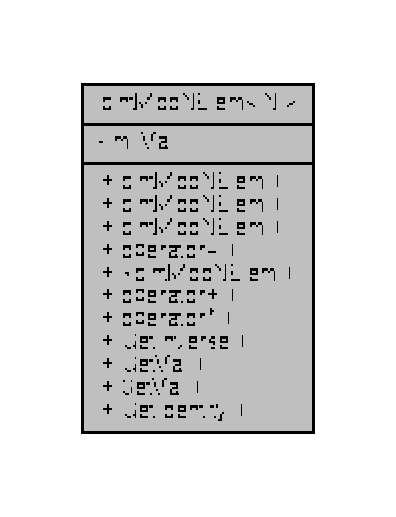
\includegraphics[width=190pt]{classcIntModNElem__coll__graph}
\end{center}
\end{figure}
\subsection*{Public Member Functions}
\begin{DoxyCompactItemize}
\item 
\hypertarget{classcIntModNElem_a93be93aa382c5501b0f36322b24e93db}{{\bfseries c\-Int\-Mod\-N\-Elem} (std\-::size\-\_\-t v)}\label{classcIntModNElem_a93be93aa382c5501b0f36322b24e93db}

\item 
\hypertarget{classcIntModNElem_a878192260976d100695404d0bbc28484}{{\bfseries c\-Int\-Mod\-N\-Elem} (const \hyperlink{classcIntModNElem}{c\-Int\-Mod\-N\-Elem} \&el)}\label{classcIntModNElem_a878192260976d100695404d0bbc28484}

\item 
\hypertarget{classcIntModNElem_a0d0ae718c816556da6fcbf19454c676d}{\hyperlink{classcIntModNElem}{Self\-Type} \& {\bfseries operator=} (const \hyperlink{classcIntModNElem}{Self\-Type} \&intmodn)}\label{classcIntModNElem_a0d0ae718c816556da6fcbf19454c676d}

\item 
\hypertarget{classcIntModNElem_a10093e22457346b333e45f1414739497}{\hyperlink{classcIntModNElem}{Self\-Type} {\bfseries operator+} (const \hyperlink{classcIntModNElem}{Self\-Type} \&a) const }\label{classcIntModNElem_a10093e22457346b333e45f1414739497}

\item 
\hypertarget{classcIntModNElem_adff6836b0b7a20c50b6b9696aea66ca6}{\hyperlink{classcIntModNElem}{Self\-Type} {\bfseries operator$\ast$} (const \hyperlink{classcIntModNElem}{Self\-Type} \&a) const }\label{classcIntModNElem_adff6836b0b7a20c50b6b9696aea66ca6}

\item 
\hypertarget{classcIntModNElem_a641e400e55b454c2832262eabc8442b6}{\hyperlink{classcIntModNElem}{Self\-Type} {\bfseries Get\-Inverse} () const }\label{classcIntModNElem_a641e400e55b454c2832262eabc8442b6}

\item 
\hypertarget{classcIntModNElem_ad584ee8c4e7e57a16963e6cb5cd73c6d}{std\-::size\-\_\-t {\bfseries Get\-Val} () const }\label{classcIntModNElem_ad584ee8c4e7e57a16963e6cb5cd73c6d}

\item 
\hypertarget{classcIntModNElem_ac5d61d5866718ab5062d5030ac44b49e}{void {\bfseries Set\-Val} (std\-::size\-\_\-t val)}\label{classcIntModNElem_ac5d61d5866718ab5062d5030ac44b49e}

\end{DoxyCompactItemize}
\subsection*{Static Public Member Functions}
\begin{DoxyCompactItemize}
\item 
\hypertarget{classcIntModNElem_a5130425382c5a5bdfd28f3b7742a4878}{{\footnotesize template$<$typename O\-P $>$ }\\static \hyperlink{classcIntModNElem}{Self\-Type} {\bfseries Get\-Identity} (O\-P Binary\-Op)}\label{classcIntModNElem_a5130425382c5a5bdfd28f3b7742a4878}

\end{DoxyCompactItemize}
\subsection*{Private Types}
\begin{DoxyCompactItemize}
\item 
\hypertarget{classcIntModNElem_ae78e9df5cc365eb679d0007191f86424}{typedef \hyperlink{classcIntModNElem}{c\-Int\-Mod\-N\-Elem}$<$ N $>$ {\bfseries Self\-Type}}\label{classcIntModNElem_ae78e9df5cc365eb679d0007191f86424}

\end{DoxyCompactItemize}
\subsection*{Private Attributes}
\begin{DoxyCompactItemize}
\item 
\hypertarget{classcIntModNElem_abaf8f2803c5a508b807c7e142da41b51}{std\-::size\-\_\-t {\bfseries m\-\_\-\-Val}}\label{classcIntModNElem_abaf8f2803c5a508b807c7e142da41b51}

\end{DoxyCompactItemize}
\subsection*{Friends}
\begin{DoxyCompactItemize}
\item 
\hypertarget{classcIntModNElem_ac999b0fda4f712c41d0a8f38c4584a8d}{std\-::ostream \& {\bfseries operator$<$$<$} (std\-::ostream \&of, const \hyperlink{classcIntModNElem}{Self\-Type} \&intmodn)}\label{classcIntModNElem_ac999b0fda4f712c41d0a8f38c4584a8d}

\end{DoxyCompactItemize}


The documentation for this class was generated from the following file\-:\begin{DoxyCompactItemize}
\item 
intmodn.\-h\end{DoxyCompactItemize}

\hypertarget{classcLinEqSys}{\section{c\-Lin\-Eq\-Sys$<$ T $>$ Class Template Reference}
\label{classcLinEqSys}\index{c\-Lin\-Eq\-Sys$<$ T $>$@{c\-Lin\-Eq\-Sys$<$ T $>$}}
}


{\ttfamily \#include $<$lineqsys.\-h$>$}



Collaboration diagram for c\-Lin\-Eq\-Sys$<$ T $>$\-:
\subsection*{Public Member Functions}
\begin{DoxyCompactItemize}
\item 
\hypertarget{classcLinEqSys_ab80e0ee1bf57383bd6b04c8e5878eeed}{{\bfseries c\-Lin\-Eq\-Sys} (const T $\ast$$\ast$elems, std\-::size\-\_\-t rows, std\-::size\-\_\-t cols)}\label{classcLinEqSys_ab80e0ee1bf57383bd6b04c8e5878eeed}

\item 
\hypertarget{classcLinEqSys_aee02a711deb23dfd1ce69bfaa06bd257}{{\bfseries c\-Lin\-Eq\-Sys} (bnu\-::matrix$<$ T $>$ \&mat)}\label{classcLinEqSys_aee02a711deb23dfd1ce69bfaa06bd257}

\item 
bnu\-::vector$<$ T $>$ \& \hyperlink{classcLinEqSys_a39978bcfd4366712d09e7eb54bb09cef}{Solve\-Unique} ()
\item 
bnu\-::vector$<$ T $>$ \hyperlink{classcLinEqSys_ad3d9edcf200c3256220054f5ee0fdaeb}{Solve\-Overdetermined} ()
\item 
bool \hyperlink{classcLinEqSys_a7144d697d601517aead8642f5956a9b0}{Solve\-Underdetermined} (std\-::vector$<$ T $>$ \&solution)
\end{DoxyCompactItemize}
\subsection*{Private Attributes}
\begin{DoxyCompactItemize}
\item 
\hypertarget{classcLinEqSys_ac270e6753af6ee64fb101b2f487ea492}{bnu\-::matrix$<$ T $>$ {\bfseries m\-\_\-\-Coeff\-Matrix}}\label{classcLinEqSys_ac270e6753af6ee64fb101b2f487ea492}

\item 
\hypertarget{classcLinEqSys_ae6d53e781615a0819bc144adb2f35d77}{bnu\-::vector$<$ T $>$ {\bfseries m\-\_\-\-Constant\-Term\-Vec}}\label{classcLinEqSys_ae6d53e781615a0819bc144adb2f35d77}

\end{DoxyCompactItemize}


\subsection{Detailed Description}
\subsubsection*{template$<$typename T$>$class c\-Lin\-Eq\-Sys$<$ T $>$}

solves a system of linear equations given as an augmented matrix 

\subsection{Member Function Documentation}
\hypertarget{classcLinEqSys_ad3d9edcf200c3256220054f5ee0fdaeb}{\index{c\-Lin\-Eq\-Sys@{c\-Lin\-Eq\-Sys}!Solve\-Overdetermined@{Solve\-Overdetermined}}
\index{Solve\-Overdetermined@{Solve\-Overdetermined}!cLinEqSys@{c\-Lin\-Eq\-Sys}}
\subsubsection[{Solve\-Overdetermined}]{\setlength{\rightskip}{0pt plus 5cm}template$<$typename T $>$ bnu\-::vector$<$T$>$ {\bf c\-Lin\-Eq\-Sys}$<$ T $>$\-::Solve\-Overdetermined (
\begin{DoxyParamCaption}
{}
\end{DoxyParamCaption}
)\hspace{0.3cm}{\ttfamily [inline]}}}\label{classcLinEqSys_ad3d9edcf200c3256220054f5ee0fdaeb}
solve an overdetermined linear system by solving the least squares problem we get an approximate solution x = (trans(\-A) $\ast$ A)$^\wedge$-\/1 $\ast$ A $\ast$ y T\-O\-D\-O -- improve on complexity -\/ this is overkill \hypertarget{classcLinEqSys_a7144d697d601517aead8642f5956a9b0}{\index{c\-Lin\-Eq\-Sys@{c\-Lin\-Eq\-Sys}!Solve\-Underdetermined@{Solve\-Underdetermined}}
\index{Solve\-Underdetermined@{Solve\-Underdetermined}!cLinEqSys@{c\-Lin\-Eq\-Sys}}
\subsubsection[{Solve\-Underdetermined}]{\setlength{\rightskip}{0pt plus 5cm}template$<$typename T $>$ bool {\bf c\-Lin\-Eq\-Sys}$<$ T $>$\-::Solve\-Underdetermined (
\begin{DoxyParamCaption}
\item[{std\-::vector$<$ T $>$ \&}]{solution}
\end{DoxyParamCaption}
)\hspace{0.3cm}{\ttfamily [inline]}}}\label{classcLinEqSys_a7144d697d601517aead8642f5956a9b0}
solve an underdetermined linear system using Singular Value Decomposition \hypertarget{classcLinEqSys_a39978bcfd4366712d09e7eb54bb09cef}{\index{c\-Lin\-Eq\-Sys@{c\-Lin\-Eq\-Sys}!Solve\-Unique@{Solve\-Unique}}
\index{Solve\-Unique@{Solve\-Unique}!cLinEqSys@{c\-Lin\-Eq\-Sys}}
\subsubsection[{Solve\-Unique}]{\setlength{\rightskip}{0pt plus 5cm}template$<$typename T $>$ bnu\-::vector$<$T$>$\& {\bf c\-Lin\-Eq\-Sys}$<$ T $>$\-::Solve\-Unique (
\begin{DoxyParamCaption}
{}
\end{DoxyParamCaption}
)\hspace{0.3cm}{\ttfamily [inline]}}}\label{classcLinEqSys_a39978bcfd4366712d09e7eb54bb09cef}
solve the linear system when there is a unique solution uses L\-U\-P factorization followed by back substitution 

The documentation for this class was generated from the following file\-:\begin{DoxyCompactItemize}
\item 
lineqsys.\-h\end{DoxyCompactItemize}

\hypertarget{classComposition}{\section{Composition Class Reference}
\label{classComposition}\index{Composition@{Composition}}
}


{\ttfamily \#include $<$binary\-\_\-op.\-h$>$}



Collaboration diagram for Composition\-:
\subsection*{Public Member Functions}
\begin{DoxyCompactItemize}
\item 
\hypertarget{classComposition_a048fe922128d64e0ac28f59ee3dd6206}{{\footnotesize template$<$typename T $>$ }\\T {\bfseries operator()} (const T \&ob1, const T \&ob2) const }\label{classComposition_a048fe922128d64e0ac28f59ee3dd6206}

\item 
\hypertarget{classComposition_a0c873693a12490e1717a280766eec6c9}{bool {\bfseries operator==} (const \hyperlink{classComposition}{Composition} \&comp) const }\label{classComposition_a0c873693a12490e1717a280766eec6c9}

\end{DoxyCompactItemize}
\subsection*{Static Public Attributes}
\begin{DoxyCompactItemize}
\item 
\hypertarget{classComposition_a3a184cd6b55d3e5cf4f86868d3350c89}{static const bool {\bfseries is\-Additive} = false}\label{classComposition_a3a184cd6b55d3e5cf4f86868d3350c89}

\item 
\hypertarget{classComposition_a4092be14bb95792e50a3670e46455b58}{static const bool {\bfseries is\-Multiplicative} = false}\label{classComposition_a4092be14bb95792e50a3670e46455b58}

\item 
\hypertarget{classComposition_ad088137e0a459dadd3a3c5b89ecdf1d1}{static const bool {\bfseries is\-Composition} = true}\label{classComposition_ad088137e0a459dadd3a3c5b89ecdf1d1}

\end{DoxyCompactItemize}


\subsection{Detailed Description}
class that represents the composition binary operation used also as a template policy 

The documentation for this class was generated from the following file\-:\begin{DoxyCompactItemize}
\item 
binary\-\_\-op.\-h\end{DoxyCompactItemize}

\hypertarget{classcPermElem}{\section{c\-Perm\-Elem \-Class \-Reference}
\label{classcPermElem}\index{c\-Perm\-Elem@{c\-Perm\-Elem}}
}


{\ttfamily \#include $<$permutation.\-h$>$}



\-Collaboration diagram for c\-Perm\-Elem\-:
\nopagebreak
\begin{figure}[H]
\begin{center}
\leavevmode
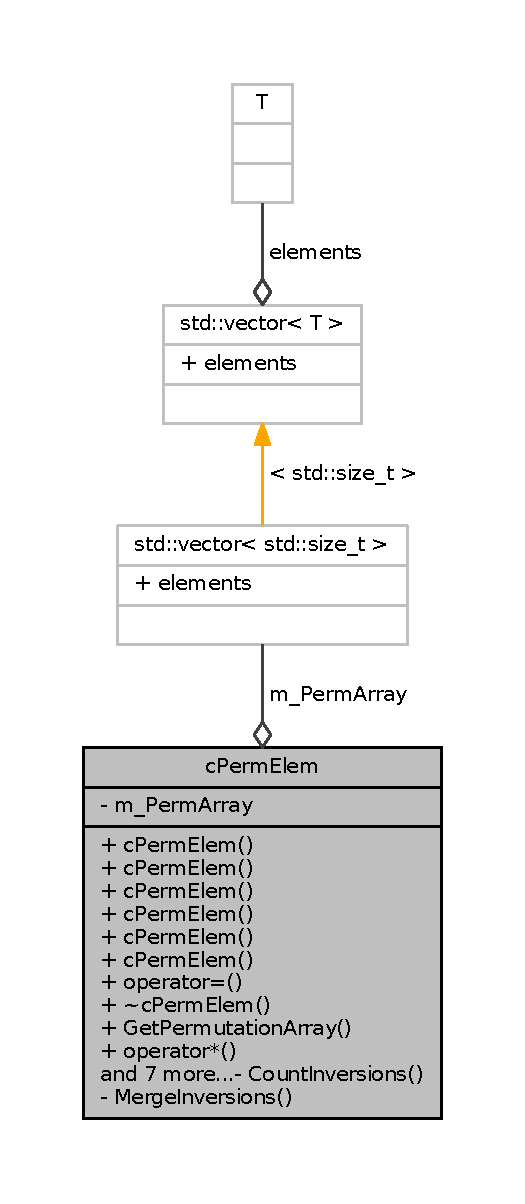
\includegraphics[height=550pt]{classcPermElem__coll__graph}
\end{center}
\end{figure}
\subsection*{\-Public \-Member \-Functions}
\begin{DoxyCompactItemize}
\item 
\hyperlink{classcPermElem_a9170fa558dd3cdfae7879631db41235d}{c\-Perm\-Elem} ()
\item 
\hyperlink{classcPermElem_ad3ff2e93580acca710249f0eb7e04bc3}{c\-Perm\-Elem} (std\-::size\-\_\-t size)
\item 
\hyperlink{classcPermElem_a375e3da4877dd48e93ca192bfcd66ddd}{c\-Perm\-Elem} (std\-::size\-\_\-t size, const std\-::initializer\-\_\-list$<$ std\-::size\-\_\-t $>$ \&perm\-\_\-sq)
\item 
\hyperlink{classcPermElem_a88b976442227c8da9ede9cf9d3f865c5}{c\-Perm\-Elem} (const std\-::initializer\-\_\-list$<$ std\-::size\-\_\-t $>$ \&perm\-\_\-sq)
\item 
\hyperlink{classcPermElem_a05895c11888d83bc3d35b3c18d90e8e4}{c\-Perm\-Elem} (std\-::vector$<$ std\-::size\-\_\-t $>$ \&perm\-\_\-sq)
\item 
\hyperlink{classcPermElem_a9cdd0f485986e63a7a848a058aecf402}{c\-Perm\-Elem} (const \hyperlink{classcPermElem}{c\-Perm\-Elem} \&permutation)
\item 
\hypertarget{classcPermElem_a9c05e75d5c9ce57fafc2cee73e396a58}{\hyperlink{classcPermElem}{c\-Perm\-Elem} \& {\bfseries operator=} (const \hyperlink{classcPermElem}{c\-Perm\-Elem} \&permutation)}\label{classcPermElem_a9c05e75d5c9ce57fafc2cee73e396a58}

\item 
std\-::vector$<$ std\-::size\-\_\-t $>$ $\ast$ \hyperlink{classcPermElem_a0d0bfc94a1d7cf92d514293253acf8be}{\-Get\-Permutation\-Array} () const 
\item 
\hyperlink{classcPermElem}{c\-Perm\-Elem} \hyperlink{classcPermElem_a19da6e521f8adf3d252250f3836c563e}{operator$\ast$} (const \hyperlink{classcPermElem}{c\-Perm\-Elem} \&perm) const 
\item 
\hypertarget{classcPermElem_a925aac2e4ac73ec288b7a1e16b941d40}{bool {\bfseries operator==} (const \hyperlink{classcPermElem}{c\-Perm\-Elem} \&perm) const }\label{classcPermElem_a925aac2e4ac73ec288b7a1e16b941d40}

\item 
\hypertarget{classcPermElem_a925cdee12dcc4914417143a88d91c49d}{bool {\bfseries operator!=} (const \hyperlink{classcPermElem}{c\-Perm\-Elem} \&perm) const }\label{classcPermElem_a925cdee12dcc4914417143a88d91c49d}

\item 
std\-::size\-\_\-t \hyperlink{classcPermElem_adad3b042383cf3538bfec790188987c3}{\-Get\-Image} (const std\-::size\-\_\-t set\-\_\-element) const 
\item 
\hyperlink{classcPermElem}{c\-Perm\-Elem} \hyperlink{classcPermElem_adbb23b8a368e0d01cd2b450ad0be5efb}{\-Get\-Mult\-Inverse} () const 
\item 
\hyperlink{classcPermElem}{c\-Perm\-Elem} \hyperlink{classcPermElem_a11cc987f70282d2984c04c6e058c41e8}{\-Get\-Ad\-Inverse} () const 
\item 
\hypertarget{classcPermElem_a773fc9acee08d4c86d391439574eaf3e}{std\-::size\-\_\-t {\bfseries \-Get\-Size} () const }\label{classcPermElem_a773fc9acee08d4c86d391439574eaf3e}

\item 
{\footnotesize template$<$typename B\-I\-N\-O\-P $>$ }\\\hyperlink{classcPermElem}{c\-Perm\-Elem} \hyperlink{classcPermElem_a7f5392e3279b766d5f85c01d363c2941}{\-Get\-Identity} (\-B\-I\-N\-O\-P binop) const 
\item 
std\-::size\-\_\-t \hyperlink{classcPermElem_a06f75de000ad4b9524116a029800ca26}{\-Get\-Inversions} () const 
\end{DoxyCompactItemize}
\subsection*{\-Private \-Member \-Functions}
\begin{DoxyCompactItemize}
\item 
void \hyperlink{classcPermElem_abefedad75d8175a886b30a6d36a0eb98}{\-Count\-Inversions} (std\-::vector$<$ std\-::size\-\_\-t $>$\-::iterator begin, std\-::vector$<$ std\-::size\-\_\-t $>$\-::iterator end, std\-::size\-\_\-t \&inversions) const 
\item 
void \hyperlink{classcPermElem_aa39ae9f1b4d3efd38616ff822caebbb9}{\-Merge\-Inversions} (std\-::vector$<$ std\-::size\-\_\-t $>$\-::iterator begin, std\-::vector$<$ std\-::size\-\_\-t $>$\-::iterator begin\-\_\-right, std\-::vector$<$ std\-::size\-\_\-t $>$\-::iterator end, std\-::size\-\_\-t \&inversions) const 
\end{DoxyCompactItemize}
\subsection*{\-Private \-Attributes}
\begin{DoxyCompactItemize}
\item 
\hypertarget{classcPermElem_a60fc59bfe827b07c6567a3b7a5a25726}{std\-::vector$<$ std\-::size\-\_\-t $>$ $\ast$ {\bfseries m\-\_\-\-Perm\-Array}}\label{classcPermElem_a60fc59bfe827b07c6567a3b7a5a25726}

\end{DoxyCompactItemize}
\subsection*{\-Friends}
\begin{DoxyCompactItemize}
\item 
\hypertarget{classcPermElem_a4211aa547f8e3f2dc6b44ad07f7224db}{std\-::ostream \& {\bfseries operator$<$$<$} (std\-::ostream \&of, const \hyperlink{classcPermElem}{c\-Perm\-Elem} \&perm)}\label{classcPermElem_a4211aa547f8e3f2dc6b44ad07f7224db}

\end{DoxyCompactItemize}


\subsection{\-Detailed \-Description}
class representing a permutation (element) permutation is represented internally using an array of ints 

\subsection{\-Constructor \& \-Destructor \-Documentation}
\hypertarget{classcPermElem_a9170fa558dd3cdfae7879631db41235d}{\index{c\-Perm\-Elem@{c\-Perm\-Elem}!c\-Perm\-Elem@{c\-Perm\-Elem}}
\index{c\-Perm\-Elem@{c\-Perm\-Elem}!cPermElem@{c\-Perm\-Elem}}
\subsubsection[{c\-Perm\-Elem}]{\setlength{\rightskip}{0pt plus 5cm}{\bf c\-Perm\-Elem\-::c\-Perm\-Elem} (
\begin{DoxyParamCaption}
{}
\end{DoxyParamCaption}
)\hspace{0.3cm}{\ttfamily  \mbox{[}inline\mbox{]}}}}\label{classcPermElem_a9170fa558dd3cdfae7879631db41235d}
default constructor for empty permutation \hypertarget{classcPermElem_ad3ff2e93580acca710249f0eb7e04bc3}{\index{c\-Perm\-Elem@{c\-Perm\-Elem}!c\-Perm\-Elem@{c\-Perm\-Elem}}
\index{c\-Perm\-Elem@{c\-Perm\-Elem}!cPermElem@{c\-Perm\-Elem}}
\subsubsection[{c\-Perm\-Elem}]{\setlength{\rightskip}{0pt plus 5cm}{\bf c\-Perm\-Elem\-::c\-Perm\-Elem} (
\begin{DoxyParamCaption}
\item[{std\-::size\-\_\-t}]{size}
\end{DoxyParamCaption}
)\hspace{0.3cm}{\ttfamily  \mbox{[}inline\mbox{]}}}}\label{classcPermElem_ad3ff2e93580acca710249f0eb7e04bc3}
constructor for identity permutation \hypertarget{classcPermElem_a375e3da4877dd48e93ca192bfcd66ddd}{\index{c\-Perm\-Elem@{c\-Perm\-Elem}!c\-Perm\-Elem@{c\-Perm\-Elem}}
\index{c\-Perm\-Elem@{c\-Perm\-Elem}!cPermElem@{c\-Perm\-Elem}}
\subsubsection[{c\-Perm\-Elem}]{\setlength{\rightskip}{0pt plus 5cm}{\bf c\-Perm\-Elem\-::c\-Perm\-Elem} (
\begin{DoxyParamCaption}
\item[{std\-::size\-\_\-t}]{size, }
\item[{const std\-::initializer\-\_\-list$<$ std\-::size\-\_\-t $>$ \&}]{perm\-\_\-sq}
\end{DoxyParamCaption}
)\hspace{0.3cm}{\ttfamily  \mbox{[}inline\mbox{]}}}}\label{classcPermElem_a375e3da4877dd48e93ca192bfcd66ddd}
constructor for permutation given as a cycle using initializer\-\_\-list ie. (3,\{1,3,2\}) means 1-\/$>$3 3-\/$>$2 2-\/$>$1 \hypertarget{classcPermElem_a88b976442227c8da9ede9cf9d3f865c5}{\index{c\-Perm\-Elem@{c\-Perm\-Elem}!c\-Perm\-Elem@{c\-Perm\-Elem}}
\index{c\-Perm\-Elem@{c\-Perm\-Elem}!cPermElem@{c\-Perm\-Elem}}
\subsubsection[{c\-Perm\-Elem}]{\setlength{\rightskip}{0pt plus 5cm}{\bf c\-Perm\-Elem\-::c\-Perm\-Elem} (
\begin{DoxyParamCaption}
\item[{const std\-::initializer\-\_\-list$<$ std\-::size\-\_\-t $>$ \&}]{perm\-\_\-sq}
\end{DoxyParamCaption}
)\hspace{0.3cm}{\ttfamily  \mbox{[}inline\mbox{]}}}}\label{classcPermElem_a88b976442227c8da9ede9cf9d3f865c5}
constructor for permutation given as an image using initializer\-\_\-list ie. \{2,3,1\} means 1-\/$>$2 2-\/$>$3 3-\/$>$1 \hypertarget{classcPermElem_a05895c11888d83bc3d35b3c18d90e8e4}{\index{c\-Perm\-Elem@{c\-Perm\-Elem}!c\-Perm\-Elem@{c\-Perm\-Elem}}
\index{c\-Perm\-Elem@{c\-Perm\-Elem}!cPermElem@{c\-Perm\-Elem}}
\subsubsection[{c\-Perm\-Elem}]{\setlength{\rightskip}{0pt plus 5cm}{\bf c\-Perm\-Elem\-::c\-Perm\-Elem} (
\begin{DoxyParamCaption}
\item[{std\-::vector$<$ std\-::size\-\_\-t $>$ \&}]{perm\-\_\-sq}
\end{DoxyParamCaption}
)\hspace{0.3cm}{\ttfamily  \mbox{[}inline\mbox{]}}}}\label{classcPermElem_a05895c11888d83bc3d35b3c18d90e8e4}
constructor for permutation given as an image using a vector ie. vector a = \{2,3,1\} is the permutation 1-\/$>$2 2-\/$>$3 3-\/$>$1 \hypertarget{classcPermElem_a9cdd0f485986e63a7a848a058aecf402}{\index{c\-Perm\-Elem@{c\-Perm\-Elem}!c\-Perm\-Elem@{c\-Perm\-Elem}}
\index{c\-Perm\-Elem@{c\-Perm\-Elem}!cPermElem@{c\-Perm\-Elem}}
\subsubsection[{c\-Perm\-Elem}]{\setlength{\rightskip}{0pt plus 5cm}{\bf c\-Perm\-Elem\-::c\-Perm\-Elem} (
\begin{DoxyParamCaption}
\item[{const {\bf c\-Perm\-Elem} \&}]{permutation}
\end{DoxyParamCaption}
)\hspace{0.3cm}{\ttfamily  \mbox{[}inline\mbox{]}}}}\label{classcPermElem_a9cdd0f485986e63a7a848a058aecf402}
copy constructor and assignment operator 

\-Here is the call graph for this function\-:
\nopagebreak
\begin{figure}[H]
\begin{center}
\leavevmode
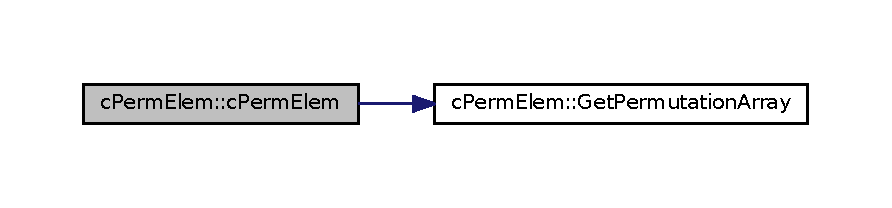
\includegraphics[width=350pt]{classcPermElem_a9cdd0f485986e63a7a848a058aecf402_cgraph}
\end{center}
\end{figure}




\subsection{\-Member \-Function \-Documentation}
\hypertarget{classcPermElem_abefedad75d8175a886b30a6d36a0eb98}{\index{c\-Perm\-Elem@{c\-Perm\-Elem}!\-Count\-Inversions@{\-Count\-Inversions}}
\index{\-Count\-Inversions@{\-Count\-Inversions}!cPermElem@{c\-Perm\-Elem}}
\subsubsection[{\-Count\-Inversions}]{\setlength{\rightskip}{0pt plus 5cm}void {\bf c\-Perm\-Elem\-::\-Count\-Inversions} (
\begin{DoxyParamCaption}
\item[{std\-::vector$<$ std\-::size\-\_\-t $>$\-::iterator}]{begin, }
\item[{std\-::vector$<$ std\-::size\-\_\-t $>$\-::iterator}]{end, }
\item[{std\-::size\-\_\-t \&}]{inversions}
\end{DoxyParamCaption}
) const\hspace{0.3cm}{\ttfamily  \mbox{[}inline, private\mbox{]}}}}\label{classcPermElem_abefedad75d8175a886b30a6d36a0eb98}
helper function for \-Get\-Inversions -\/-\/ modified merge sort \-Complexity\-: \-O(nlgn) 

\-Here is the call graph for this function\-:
\nopagebreak
\begin{figure}[H]
\begin{center}
\leavevmode
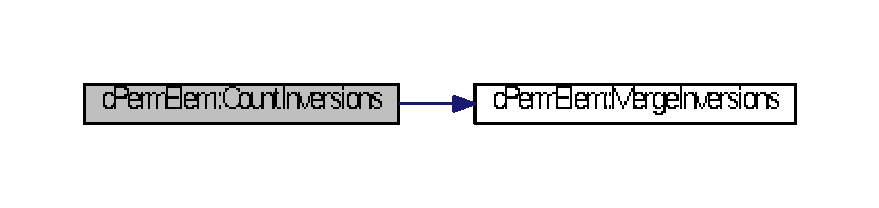
\includegraphics[width=350pt]{classcPermElem_abefedad75d8175a886b30a6d36a0eb98_cgraph}
\end{center}
\end{figure}


\hypertarget{classcPermElem_a11cc987f70282d2984c04c6e058c41e8}{\index{c\-Perm\-Elem@{c\-Perm\-Elem}!\-Get\-Ad\-Inverse@{\-Get\-Ad\-Inverse}}
\index{\-Get\-Ad\-Inverse@{\-Get\-Ad\-Inverse}!cPermElem@{c\-Perm\-Elem}}
\subsubsection[{\-Get\-Ad\-Inverse}]{\setlength{\rightskip}{0pt plus 5cm}{\bf c\-Perm\-Elem} {\bf c\-Perm\-Elem\-::\-Get\-Ad\-Inverse} (
\begin{DoxyParamCaption}
{}
\end{DoxyParamCaption}
) const\hspace{0.3cm}{\ttfamily  \mbox{[}inline\mbox{]}}}}\label{classcPermElem_a11cc987f70282d2984c04c6e058c41e8}
the same as \-Get\-Mult\-Inverse -\/-\/ defined for consistency 

\-Here is the call graph for this function\-:
\nopagebreak
\begin{figure}[H]
\begin{center}
\leavevmode
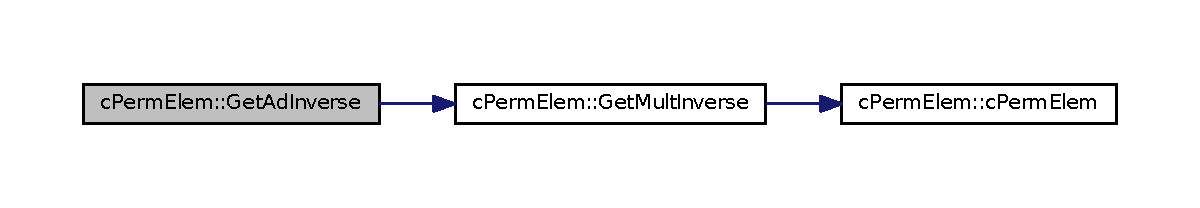
\includegraphics[width=350pt]{classcPermElem_a11cc987f70282d2984c04c6e058c41e8_cgraph}
\end{center}
\end{figure}


\hypertarget{classcPermElem_a7f5392e3279b766d5f85c01d363c2941}{\index{c\-Perm\-Elem@{c\-Perm\-Elem}!\-Get\-Identity@{\-Get\-Identity}}
\index{\-Get\-Identity@{\-Get\-Identity}!cPermElem@{c\-Perm\-Elem}}
\subsubsection[{\-Get\-Identity}]{\setlength{\rightskip}{0pt plus 5cm}template$<$typename B\-I\-N\-O\-P $>$ {\bf c\-Perm\-Elem} {\bf c\-Perm\-Elem\-::\-Get\-Identity} (
\begin{DoxyParamCaption}
\item[{\-B\-I\-N\-O\-P}]{binop}
\end{DoxyParamCaption}
) const\hspace{0.3cm}{\ttfamily  \mbox{[}inline\mbox{]}}}}\label{classcPermElem_a7f5392e3279b766d5f85c01d363c2941}
returns the identity permutation with the same size as the current permutation 

\-Here is the call graph for this function\-:
\nopagebreak
\begin{figure}[H]
\begin{center}
\leavevmode
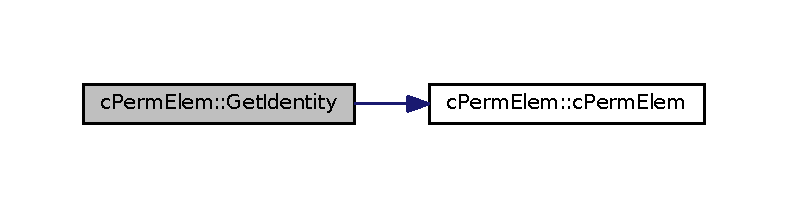
\includegraphics[width=350pt]{classcPermElem_a7f5392e3279b766d5f85c01d363c2941_cgraph}
\end{center}
\end{figure}


\hypertarget{classcPermElem_adad3b042383cf3538bfec790188987c3}{\index{c\-Perm\-Elem@{c\-Perm\-Elem}!\-Get\-Image@{\-Get\-Image}}
\index{\-Get\-Image@{\-Get\-Image}!cPermElem@{c\-Perm\-Elem}}
\subsubsection[{\-Get\-Image}]{\setlength{\rightskip}{0pt plus 5cm}std\-::size\-\_\-t {\bf c\-Perm\-Elem\-::\-Get\-Image} (
\begin{DoxyParamCaption}
\item[{const std\-::size\-\_\-t}]{set\-\_\-element}
\end{DoxyParamCaption}
) const\hspace{0.3cm}{\ttfamily  \mbox{[}inline\mbox{]}}}}\label{classcPermElem_adad3b042383cf3538bfec790188987c3}
get the image of an element under the action of the permution \hypertarget{classcPermElem_a06f75de000ad4b9524116a029800ca26}{\index{c\-Perm\-Elem@{c\-Perm\-Elem}!\-Get\-Inversions@{\-Get\-Inversions}}
\index{\-Get\-Inversions@{\-Get\-Inversions}!cPermElem@{c\-Perm\-Elem}}
\subsubsection[{\-Get\-Inversions}]{\setlength{\rightskip}{0pt plus 5cm}std\-::size\-\_\-t {\bf c\-Perm\-Elem\-::\-Get\-Inversions} (
\begin{DoxyParamCaption}
{}
\end{DoxyParamCaption}
) const\hspace{0.3cm}{\ttfamily  \mbox{[}inline\mbox{]}}}}\label{classcPermElem_a06f75de000ad4b9524116a029800ca26}
returns the number of inverses\-: \char`\"{}inverse\char`\"{} if i $<$ j and \-A\mbox{[}i\mbox{]} $>$ \-A\mbox{[}j\mbox{]} modified merge sort =$>$ \-Complexity\-: \-O(nlgn) see \-Cormen chapter 2 -\/ exercises 

\-Here is the call graph for this function\-:
\nopagebreak
\begin{figure}[H]
\begin{center}
\leavevmode
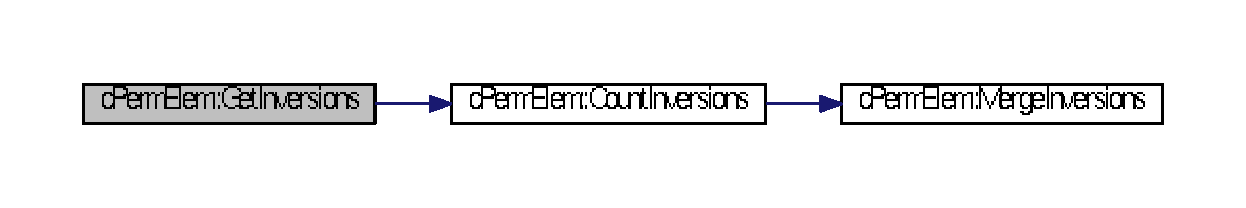
\includegraphics[width=350pt]{classcPermElem_a06f75de000ad4b9524116a029800ca26_cgraph}
\end{center}
\end{figure}


\hypertarget{classcPermElem_adbb23b8a368e0d01cd2b450ad0be5efb}{\index{c\-Perm\-Elem@{c\-Perm\-Elem}!\-Get\-Mult\-Inverse@{\-Get\-Mult\-Inverse}}
\index{\-Get\-Mult\-Inverse@{\-Get\-Mult\-Inverse}!cPermElem@{c\-Perm\-Elem}}
\subsubsection[{\-Get\-Mult\-Inverse}]{\setlength{\rightskip}{0pt plus 5cm}{\bf c\-Perm\-Elem} {\bf c\-Perm\-Elem\-::\-Get\-Mult\-Inverse} (
\begin{DoxyParamCaption}
{}
\end{DoxyParamCaption}
) const\hspace{0.3cm}{\ttfamily  \mbox{[}inline\mbox{]}}}}\label{classcPermElem_adbb23b8a368e0d01cd2b450ad0be5efb}
returns the permutation inverse \-Complexity\-: \-O(n) 

\-Here is the call graph for this function\-:
\nopagebreak
\begin{figure}[H]
\begin{center}
\leavevmode
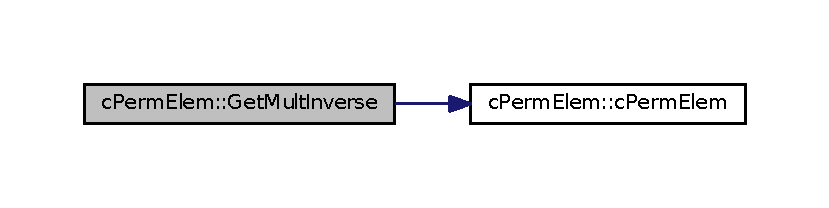
\includegraphics[width=350pt]{classcPermElem_adbb23b8a368e0d01cd2b450ad0be5efb_cgraph}
\end{center}
\end{figure}


\hypertarget{classcPermElem_a0d0bfc94a1d7cf92d514293253acf8be}{\index{c\-Perm\-Elem@{c\-Perm\-Elem}!\-Get\-Permutation\-Array@{\-Get\-Permutation\-Array}}
\index{\-Get\-Permutation\-Array@{\-Get\-Permutation\-Array}!cPermElem@{c\-Perm\-Elem}}
\subsubsection[{\-Get\-Permutation\-Array}]{\setlength{\rightskip}{0pt plus 5cm}std\-::vector$<$std\-::size\-\_\-t$>$$\ast$ {\bf c\-Perm\-Elem\-::\-Get\-Permutation\-Array} (
\begin{DoxyParamCaption}
{}
\end{DoxyParamCaption}
) const\hspace{0.3cm}{\ttfamily  \mbox{[}inline\mbox{]}}}}\label{classcPermElem_a0d0bfc94a1d7cf92d514293253acf8be}
get the underlying permutation array \hypertarget{classcPermElem_aa39ae9f1b4d3efd38616ff822caebbb9}{\index{c\-Perm\-Elem@{c\-Perm\-Elem}!\-Merge\-Inversions@{\-Merge\-Inversions}}
\index{\-Merge\-Inversions@{\-Merge\-Inversions}!cPermElem@{c\-Perm\-Elem}}
\subsubsection[{\-Merge\-Inversions}]{\setlength{\rightskip}{0pt plus 5cm}void {\bf c\-Perm\-Elem\-::\-Merge\-Inversions} (
\begin{DoxyParamCaption}
\item[{std\-::vector$<$ std\-::size\-\_\-t $>$\-::iterator}]{begin, }
\item[{std\-::vector$<$ std\-::size\-\_\-t $>$\-::iterator}]{begin\-\_\-right, }
\item[{std\-::vector$<$ std\-::size\-\_\-t $>$\-::iterator}]{end, }
\item[{std\-::size\-\_\-t \&}]{inversions}
\end{DoxyParamCaption}
) const\hspace{0.3cm}{\ttfamily  \mbox{[}inline, private\mbox{]}}}}\label{classcPermElem_aa39ae9f1b4d3efd38616ff822caebbb9}
equivalent to merge procedure from merge sort \-Complexity\-: \-O(n) \hypertarget{classcPermElem_a19da6e521f8adf3d252250f3836c563e}{\index{c\-Perm\-Elem@{c\-Perm\-Elem}!operator$\ast$@{operator$\ast$}}
\index{operator$\ast$@{operator$\ast$}!cPermElem@{c\-Perm\-Elem}}
\subsubsection[{operator$\ast$}]{\setlength{\rightskip}{0pt plus 5cm}{\bf c\-Perm\-Elem} c\-Perm\-Elem\-::operator$\ast$ (
\begin{DoxyParamCaption}
\item[{const {\bf c\-Perm\-Elem} \&}]{perm}
\end{DoxyParamCaption}
) const\hspace{0.3cm}{\ttfamily  \mbox{[}inline\mbox{]}}}}\label{classcPermElem_a19da6e521f8adf3d252250f3836c563e}
permutation mutiplication operator (doesn't work in the true mathematical meaning of composition-\/-\/ aplies the first permutation first\-: \-A$\ast$\-B(x) -\/$>$ \-B(\-A(x)) ) \-Complexity\-: \-O(n) 

\-Here is the call graph for this function\-:
\nopagebreak
\begin{figure}[H]
\begin{center}
\leavevmode
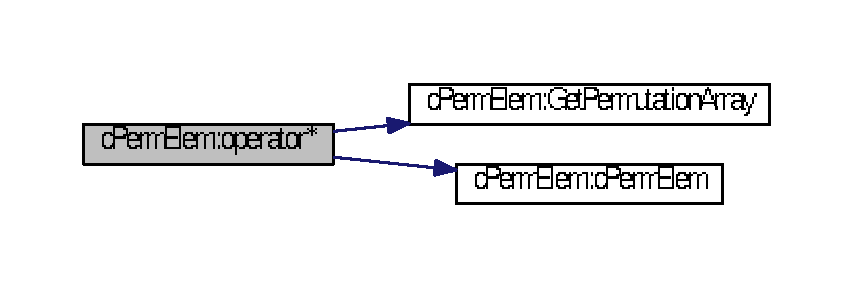
\includegraphics[width=350pt]{classcPermElem_a19da6e521f8adf3d252250f3836c563e_cgraph}
\end{center}
\end{figure}




\-The documentation for this class was generated from the following file\-:\begin{DoxyCompactItemize}
\item 
permutation.\-h\end{DoxyCompactItemize}

\hypertarget{classcSLPRep}{
\section{c\-S\-L\-P\-Rep$<$ \-T $>$ \-Class \-Template \-Reference}
\label{classcSLPRep}\index{c\-S\-L\-P\-Rep$<$ T $>$@{c\-S\-L\-P\-Rep$<$ T $>$}}
}
\subsection*{\-Private \-Member \-Functions}
\begin{DoxyCompactItemize}
\item 
\hypertarget{classcSLPRep_a426437f339e324639960d31d80a88c16}{
void {\bfseries \-Evaluate\-S\-L\-P} () const }
\label{classcSLPRep_a426437f339e324639960d31d80a88c16}

\end{DoxyCompactItemize}
\subsection*{\-Private \-Attributes}
\begin{DoxyCompactItemize}
\item 
\hypertarget{classcSLPRep_a5da028fd67619a049145140669a44eb1}{
std\-::size\-\_\-t {\bfseries m\-\_\-\-Rank}}
\label{classcSLPRep_a5da028fd67619a049145140669a44eb1}

\item 
\hypertarget{classcSLPRep_a8545e9ddf3197b62c4cd38fbae189a26}{
std\-::vector$<$ \-T $>$ {\bfseries m\-\_\-\-S\-L\-P}}
\label{classcSLPRep_a8545e9ddf3197b62c4cd38fbae189a26}

\end{DoxyCompactItemize}
\subsubsection*{template$<$typename T$>$ class c\-S\-L\-P\-Rep$<$ T $>$}



\-The documentation for this class was generated from the following file\-:\begin{DoxyCompactItemize}
\item 
slp\-\_\-rep.\-h\end{DoxyCompactItemize}

\hypertarget{classcSubgroup}{\section{c\-Subgroup$<$ G $>$ Class Template Reference}
\label{classcSubgroup}\index{c\-Subgroup$<$ G $>$@{c\-Subgroup$<$ G $>$}}
}


Inheritance diagram for c\-Subgroup$<$ G $>$\-:
\nopagebreak
\begin{figure}[H]
\begin{center}
\leavevmode
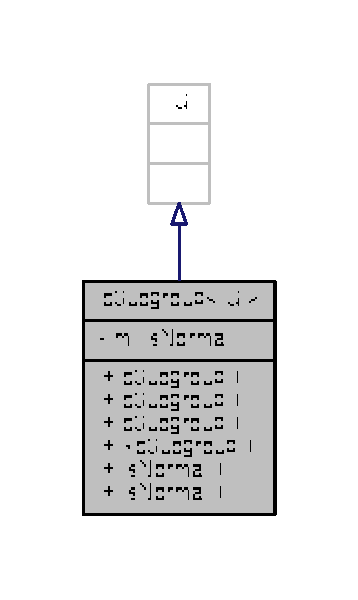
\includegraphics[width=172pt]{classcSubgroup__inherit__graph}
\end{center}
\end{figure}


Collaboration diagram for c\-Subgroup$<$ G $>$\-:
\nopagebreak
\begin{figure}[H]
\begin{center}
\leavevmode
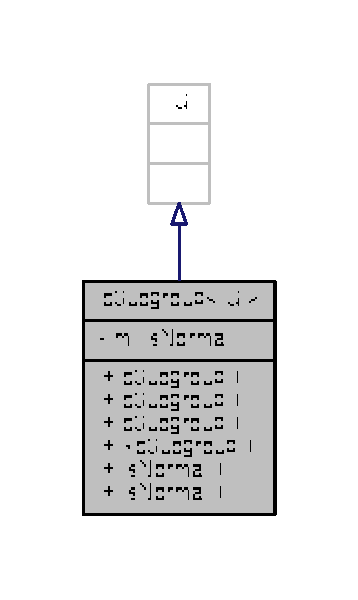
\includegraphics[width=172pt]{classcSubgroup__coll__graph}
\end{center}
\end{figure}
\subsection*{Public Types}
\begin{DoxyCompactItemize}
\item 
\hypertarget{classcSubgroup_ab88b056e488e5b0b6c7849e9a4357371}{typedef G\-::\-Element\-Type {\bfseries T}}\label{classcSubgroup_ab88b056e488e5b0b6c7849e9a4357371}

\end{DoxyCompactItemize}
\subsection*{Public Member Functions}
\begin{DoxyCompactItemize}
\item 
\hypertarget{classcSubgroup_aa47db239ee5fc0c2904fc5870e102daa}{{\bfseries c\-Subgroup} (std\-::vector$<$ T $>$ gr\-\_\-vec)}\label{classcSubgroup_aa47db239ee5fc0c2904fc5870e102daa}

\item 
\hypertarget{classcSubgroup_ad10d7eaf034a3f96bfdb84e824f7ba30}{{\bfseries c\-Subgroup} (G \&group)}\label{classcSubgroup_ad10d7eaf034a3f96bfdb84e824f7ba30}

\item 
\hypertarget{classcSubgroup_a5c239313a0f1ae9ae64f87da3c552bee}{bool {\bfseries is\-Normal} () const }\label{classcSubgroup_a5c239313a0f1ae9ae64f87da3c552bee}

\item 
\hypertarget{classcSubgroup_a39fa2b6d316997d9ecbb2fc51cf86bc6}{void {\bfseries is\-Normal} (const bool normal)}\label{classcSubgroup_a39fa2b6d316997d9ecbb2fc51cf86bc6}

\end{DoxyCompactItemize}
\subsection*{Private Attributes}
\begin{DoxyCompactItemize}
\item 
\hypertarget{classcSubgroup_a21daac84974df25a48465da9438cb552}{bool {\bfseries m\-\_\-is\-Normal}}\label{classcSubgroup_a21daac84974df25a48465da9438cb552}

\end{DoxyCompactItemize}


The documentation for this class was generated from the following file\-:\begin{DoxyCompactItemize}
\item 
subgroup.\-h\end{DoxyCompactItemize}

\hypertarget{classcSymmetricRep}{\section{c\-Symmetric\-Rep$<$ T $>$ Class Template Reference}
\label{classcSymmetricRep}\index{c\-Symmetric\-Rep$<$ T $>$@{c\-Symmetric\-Rep$<$ T $>$}}
}


{\ttfamily \#include $<$symmetric\-\_\-rep.\-h$>$}



Collaboration diagram for c\-Symmetric\-Rep$<$ T $>$\-:
\subsection*{Public Types}
\begin{DoxyCompactItemize}
\item 
\hypertarget{classcSymmetricRep_abb21d3323b4e2133ec7bbc4f2d45d968}{typedef \hyperlink{classcSymmetricRep}{c\-Symmetric\-Rep}$<$ T $>$ {\bfseries Self\-Type}}\label{classcSymmetricRep_abb21d3323b4e2133ec7bbc4f2d45d968}

\end{DoxyCompactItemize}
\subsection*{Public Member Functions}
\begin{DoxyCompactItemize}
\item 
\hyperlink{classcSymmetricRep_a64f4c25b8f5aebbd78f49f3485aed88f}{c\-Symmetric\-Rep} (std\-::vector$<$ T $>$ \&generators\-\_\-set)
\item 
\hyperlink{classcSymmetricRep_a47ba133fe6f1ba2b8d3da5ae6cb001d9}{c\-Symmetric\-Rep} (std\-::initializer\-\_\-list$<$ T $>$ perm\-\_\-list)
\item 
\hypertarget{classcSymmetricRep_a5fa8e9aabcacfddbf5f8d896a9bf6c94}{{\bfseries c\-Symmetric\-Rep} (const \hyperlink{classcSymmetricRep}{Self\-Type} \&sym\-\_\-rep)}\label{classcSymmetricRep_a5fa8e9aabcacfddbf5f8d896a9bf6c94}

\item 
\hypertarget{classcSymmetricRep_a42ce2132ef0a6c51f7afc4496c121cbe}{\hyperlink{classcSymmetricRep}{c\-Symmetric\-Rep} \& {\bfseries operator=} (const \hyperlink{classcSymmetricRep}{Self\-Type} \&sym\-\_\-rep)}\label{classcSymmetricRep_a42ce2132ef0a6c51f7afc4496c121cbe}

\item 
bool \hyperlink{classcSymmetricRep_a60f095284b40e494a34fda76e1fc7ecd}{Contains} (const T \&element) const 
\item 
std\-::vector$<$ T $>$ \hyperlink{classcSymmetricRep_a935cec1dbd90a09581f1aa7f150eb9de}{Get\-Elements\-Naive} () const 
\item 
std\-::vector$<$ T $>$ \hyperlink{classcSymmetricRep_ad9f112b996c14824bd1d669aed162cbf}{Get\-Elements\-Dimino} () const 
\item 
std\-::vector$<$ std\-::size\-\_\-t $>$ \hyperlink{classcSymmetricRep_a62cbd7057456f503eec43d592497e94f}{Get\-Orbit} (const std\-::size\-\_\-t \&set\-\_\-element) const 
\item 
\hypertarget{classcSymmetricRep_af90591a8af82e61668da036efa04a5fd}{const std\-::vector$<$ T $>$ \& {\bfseries Get\-Generators\-Set} () const }\label{classcSymmetricRep_af90591a8af82e61668da036efa04a5fd}

\item 
\hypertarget{classcSymmetricRep_a10df8259eeafac4f03c8d7b251f37dfb}{void {\bfseries Set\-Generators\-Set} (const std\-::vector$<$ T $>$ \&gen\-\_\-set)}\label{classcSymmetricRep_a10df8259eeafac4f03c8d7b251f37dfb}

\item 
\hypertarget{classcSymmetricRep_a59125541fe5801e2073cacb54ed879d8}{void {\bfseries Add\-Generator} (const T \&element)}\label{classcSymmetricRep_a59125541fe5801e2073cacb54ed879d8}

\item 
\hypertarget{classcSymmetricRep_a37c8cab52b7ef4aa4b83f3ef203036ef}{void {\bfseries Clear\-Generators} ()}\label{classcSymmetricRep_a37c8cab52b7ef4aa4b83f3ef203036ef}

\item 
\hypertarget{classcSymmetricRep_a30639c704b01408475c9fd4a100d738d}{bool {\bfseries operator==} (const \hyperlink{classcSymmetricRep}{Self\-Type} \&symgrp) const }\label{classcSymmetricRep_a30639c704b01408475c9fd4a100d738d}

\item 
\hypertarget{classcSymmetricRep_a77bcf4f11ff92c57aa6626c075bf3355}{bool {\bfseries operator!=} (const \hyperlink{classcSymmetricRep}{Self\-Type} \&symgrp) const }\label{classcSymmetricRep_a77bcf4f11ff92c57aa6626c075bf3355}

\item 
\hypertarget{classcSymmetricRep_a5182c5dcf4247c03a7e0de001e7c1cf3}{T {\bfseries Get\-Identity} () const }\label{classcSymmetricRep_a5182c5dcf4247c03a7e0de001e7c1cf3}

\item 
std\-::vector$<$ T $>$ \hyperlink{classcSymmetricRep_a2dfa5d3358d69914a625536d994be72c}{Get\-Cyclic\-Subgroup\-El} (const T \&element) const 
\item 
std\-::vector$<$ T $>$ \hyperlink{classcSymmetricRep_ac110028d8d6e161448f15bc1548d5274}{Get\-Cyclic\-Subgroup\-El} (const std\-::size\-\_\-t size)
\item 
std\-::vector$<$ T $>$ \hyperlink{classcSymmetricRep_a4a9724dc8ba8c8ccc041fe1f86dc4701}{Get\-Dihedral\-Subgroup\-El} (const std\-::size\-\_\-t size)
\end{DoxyCompactItemize}
\subsection*{Private Attributes}
\begin{DoxyCompactItemize}
\item 
\hypertarget{classcSymmetricRep_ab9afa5a928d6fba3c560e0245ab5d0e4}{std\-::vector$<$ T $>$ {\bfseries m\-\_\-\-Gen\-Set}}\label{classcSymmetricRep_ab9afa5a928d6fba3c560e0245ab5d0e4}

\end{DoxyCompactItemize}
\subsection*{Friends}
\begin{DoxyCompactItemize}
\item 
\hypertarget{classcSymmetricRep_ad73abea0c910e6d44cac98fd4bc1a8a8}{std\-::ostream \& {\bfseries operator$<$$<$} (std\-::ostream \&out, const \hyperlink{classcSymmetricRep}{Self\-Type} \&group\-\_\-rep)}\label{classcSymmetricRep_ad73abea0c910e6d44cac98fd4bc1a8a8}

\end{DoxyCompactItemize}


\subsection{Detailed Description}
\subsubsection*{template$<$typename T$>$class c\-Symmetric\-Rep$<$ T $>$}

symmetric group internal representation class used only from \hyperlink{classcGroup}{c\-Group} T\-O\-D\-O -- add elements member + Get\-Elements method (cache) 

\subsection{Constructor \& Destructor Documentation}
\hypertarget{classcSymmetricRep_a64f4c25b8f5aebbd78f49f3485aed88f}{\index{c\-Symmetric\-Rep@{c\-Symmetric\-Rep}!c\-Symmetric\-Rep@{c\-Symmetric\-Rep}}
\index{c\-Symmetric\-Rep@{c\-Symmetric\-Rep}!cSymmetricRep@{c\-Symmetric\-Rep}}
\subsubsection[{c\-Symmetric\-Rep}]{\setlength{\rightskip}{0pt plus 5cm}template$<$typename T $>$ {\bf c\-Symmetric\-Rep}$<$ T $>$\-::{\bf c\-Symmetric\-Rep} (
\begin{DoxyParamCaption}
\item[{std\-::vector$<$ T $>$ \&}]{generators\-\_\-set}
\end{DoxyParamCaption}
)\hspace{0.3cm}{\ttfamily [inline]}}}\label{classcSymmetricRep_a64f4c25b8f5aebbd78f49f3485aed88f}
constructs object from a vector of permutations \hypertarget{classcSymmetricRep_a47ba133fe6f1ba2b8d3da5ae6cb001d9}{\index{c\-Symmetric\-Rep@{c\-Symmetric\-Rep}!c\-Symmetric\-Rep@{c\-Symmetric\-Rep}}
\index{c\-Symmetric\-Rep@{c\-Symmetric\-Rep}!cSymmetricRep@{c\-Symmetric\-Rep}}
\subsubsection[{c\-Symmetric\-Rep}]{\setlength{\rightskip}{0pt plus 5cm}template$<$typename T $>$ {\bf c\-Symmetric\-Rep}$<$ T $>$\-::{\bf c\-Symmetric\-Rep} (
\begin{DoxyParamCaption}
\item[{std\-::initializer\-\_\-list$<$ T $>$}]{perm\-\_\-list}
\end{DoxyParamCaption}
)\hspace{0.3cm}{\ttfamily [inline]}}}\label{classcSymmetricRep_a47ba133fe6f1ba2b8d3da5ae6cb001d9}
constructs object from an intializer list of permutations 

\subsection{Member Function Documentation}
\hypertarget{classcSymmetricRep_a60f095284b40e494a34fda76e1fc7ecd}{\index{c\-Symmetric\-Rep@{c\-Symmetric\-Rep}!Contains@{Contains}}
\index{Contains@{Contains}!cSymmetricRep@{c\-Symmetric\-Rep}}
\subsubsection[{Contains}]{\setlength{\rightskip}{0pt plus 5cm}template$<$typename T $>$ bool {\bf c\-Symmetric\-Rep}$<$ T $>$\-::Contains (
\begin{DoxyParamCaption}
\item[{const T \&}]{element}
\end{DoxyParamCaption}
) const\hspace{0.3cm}{\ttfamily [inline]}}}\label{classcSymmetricRep_a60f095284b40e494a34fda76e1fc7ecd}
returns true if it finds the element in the elements obtained by running Dimino's algorithm 

Here is the call graph for this function\-:


\hypertarget{classcSymmetricRep_a2dfa5d3358d69914a625536d994be72c}{\index{c\-Symmetric\-Rep@{c\-Symmetric\-Rep}!Get\-Cyclic\-Subgroup\-El@{Get\-Cyclic\-Subgroup\-El}}
\index{Get\-Cyclic\-Subgroup\-El@{Get\-Cyclic\-Subgroup\-El}!cSymmetricRep@{c\-Symmetric\-Rep}}
\subsubsection[{Get\-Cyclic\-Subgroup\-El}]{\setlength{\rightskip}{0pt plus 5cm}template$<$typename T $>$ std\-::vector$<$T$>$ {\bf c\-Symmetric\-Rep}$<$ T $>$\-::Get\-Cyclic\-Subgroup\-El (
\begin{DoxyParamCaption}
\item[{const T \&}]{element}
\end{DoxyParamCaption}
) const\hspace{0.3cm}{\ttfamily [inline]}}}\label{classcSymmetricRep_a2dfa5d3358d69914a625536d994be72c}
returns the cyclic subgroup elements generated by the given element by computing it's powers until identity is reached Complexity\-: O(n), where n is the order of the element \hypertarget{classcSymmetricRep_ac110028d8d6e161448f15bc1548d5274}{\index{c\-Symmetric\-Rep@{c\-Symmetric\-Rep}!Get\-Cyclic\-Subgroup\-El@{Get\-Cyclic\-Subgroup\-El}}
\index{Get\-Cyclic\-Subgroup\-El@{Get\-Cyclic\-Subgroup\-El}!cSymmetricRep@{c\-Symmetric\-Rep}}
\subsubsection[{Get\-Cyclic\-Subgroup\-El}]{\setlength{\rightskip}{0pt plus 5cm}template$<$typename T $>$ std\-::vector$<$T$>$ {\bf c\-Symmetric\-Rep}$<$ T $>$\-::Get\-Cyclic\-Subgroup\-El (
\begin{DoxyParamCaption}
\item[{const std\-::size\-\_\-t}]{size}
\end{DoxyParamCaption}
)\hspace{0.3cm}{\ttfamily [inline]}}}\label{classcSymmetricRep_ac110028d8d6e161448f15bc1548d5274}
returns the cyclic subgroup \$\-C\-\_\-n\$ elements by rotating the identity permutation of the given size Complexity \$\-O(n)\$, where n is the size given as parameter \hypertarget{classcSymmetricRep_a4a9724dc8ba8c8ccc041fe1f86dc4701}{\index{c\-Symmetric\-Rep@{c\-Symmetric\-Rep}!Get\-Dihedral\-Subgroup\-El@{Get\-Dihedral\-Subgroup\-El}}
\index{Get\-Dihedral\-Subgroup\-El@{Get\-Dihedral\-Subgroup\-El}!cSymmetricRep@{c\-Symmetric\-Rep}}
\subsubsection[{Get\-Dihedral\-Subgroup\-El}]{\setlength{\rightskip}{0pt plus 5cm}template$<$typename T $>$ std\-::vector$<$T$>$ {\bf c\-Symmetric\-Rep}$<$ T $>$\-::Get\-Dihedral\-Subgroup\-El (
\begin{DoxyParamCaption}
\item[{const std\-::size\-\_\-t}]{size}
\end{DoxyParamCaption}
)\hspace{0.3cm}{\ttfamily [inline]}}}\label{classcSymmetricRep_a4a9724dc8ba8c8ccc041fe1f86dc4701}
returns the dihedral subgroup \$\-D\-\_\-2n\$ = \$\-C\-\_\-n + R\-\_\-n\$, where \$\-R\-\_\-n\$ is generated rotating by a fundamental reflection Complexity \$\-O(2n)\$, where n is the size of the symmetry n-\/gon 

Here is the call graph for this function\-:


\hypertarget{classcSymmetricRep_ad9f112b996c14824bd1d669aed162cbf}{\index{c\-Symmetric\-Rep@{c\-Symmetric\-Rep}!Get\-Elements\-Dimino@{Get\-Elements\-Dimino}}
\index{Get\-Elements\-Dimino@{Get\-Elements\-Dimino}!cSymmetricRep@{c\-Symmetric\-Rep}}
\subsubsection[{Get\-Elements\-Dimino}]{\setlength{\rightskip}{0pt plus 5cm}template$<$typename T $>$ std\-::vector$<$T$>$ {\bf c\-Symmetric\-Rep}$<$ T $>$\-::Get\-Elements\-Dimino (
\begin{DoxyParamCaption}
{}
\end{DoxyParamCaption}
) const\hspace{0.3cm}{\ttfamily [inline]}}}\label{classcSymmetricRep_ad9f112b996c14824bd1d669aed162cbf}
returns the group elements by performing the Dimino algorithm T\-O\-D\-O -\/ Complexity\-: see Butler -\/ \char`\"{}\-Fundamental Algorithms for permutation groups\char`\"{} 

Here is the call graph for this function\-:


\hypertarget{classcSymmetricRep_a935cec1dbd90a09581f1aa7f150eb9de}{\index{c\-Symmetric\-Rep@{c\-Symmetric\-Rep}!Get\-Elements\-Naive@{Get\-Elements\-Naive}}
\index{Get\-Elements\-Naive@{Get\-Elements\-Naive}!cSymmetricRep@{c\-Symmetric\-Rep}}
\subsubsection[{Get\-Elements\-Naive}]{\setlength{\rightskip}{0pt plus 5cm}template$<$typename T $>$ std\-::vector$<$T$>$ {\bf c\-Symmetric\-Rep}$<$ T $>$\-::Get\-Elements\-Naive (
\begin{DoxyParamCaption}
{}
\end{DoxyParamCaption}
) const\hspace{0.3cm}{\ttfamily [inline]}}}\label{classcSymmetricRep_a935cec1dbd90a09581f1aa7f150eb9de}
returns the set of elements by trying to generate all combinations Complexity\-: O(n$^\wedge$2$\ast$m), where n is the number of elements and m is the number of generators T\-O\-D\-O -\/ by improving the data structure we could improve the find operation see Butler -\/ \char`\"{}\-Fundamental Algorithms for permutation groups\char`\"{} \hypertarget{classcSymmetricRep_a62cbd7057456f503eec43d592497e94f}{\index{c\-Symmetric\-Rep@{c\-Symmetric\-Rep}!Get\-Orbit@{Get\-Orbit}}
\index{Get\-Orbit@{Get\-Orbit}!cSymmetricRep@{c\-Symmetric\-Rep}}
\subsubsection[{Get\-Orbit}]{\setlength{\rightskip}{0pt plus 5cm}template$<$typename T $>$ std\-::vector$<$std\-::size\-\_\-t$>$ {\bf c\-Symmetric\-Rep}$<$ T $>$\-::Get\-Orbit (
\begin{DoxyParamCaption}
\item[{const std\-::size\-\_\-t \&}]{set\-\_\-element}
\end{DoxyParamCaption}
) const\hspace{0.3cm}{\ttfamily [inline]}}}\label{classcSymmetricRep_a62cbd7057456f503eec43d592497e94f}
returns the orbit of a set element(the images of the elements under the group elements) Complexity\-: O(n$^\wedge$2$\ast$m) where n is the size of the orbit and m is the order of the group 

Here is the call graph for this function\-:




The documentation for this class was generated from the following file\-:\begin{DoxyCompactItemize}
\item 
symmetric\-\_\-rep.\-h\end{DoxyCompactItemize}

\hypertarget{classtree_1_1cThreadedRep}{\section{tree\-:\-:c\-Threaded\-Rep$<$ \-T $>$ \-Class \-Template \-Reference}
\label{classtree_1_1cThreadedRep}\index{tree\-::c\-Threaded\-Rep$<$ T $>$@{tree\-::c\-Threaded\-Rep$<$ T $>$}}
}


{\ttfamily \#include $<$threaded\-\_\-rep.\-h$>$}



\-Collaboration diagram for tree\-:\-:c\-Threaded\-Rep$<$ \-T $>$\-:
\nopagebreak
\begin{figure}[H]
\begin{center}
\leavevmode
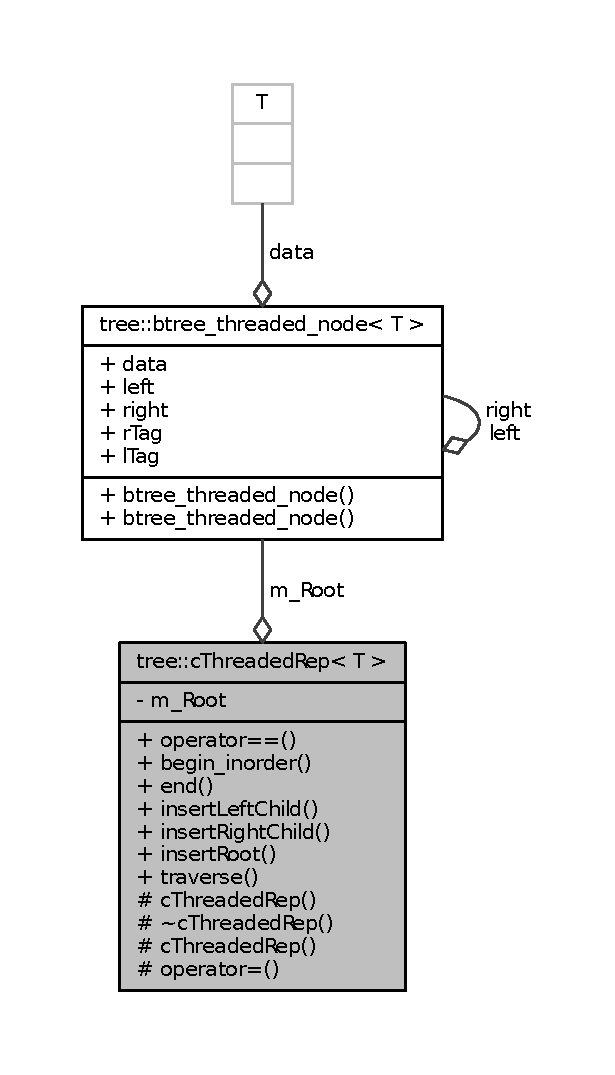
\includegraphics[width=295pt]{classtree_1_1cThreadedRep__coll__graph}
\end{center}
\end{figure}
\subsection*{\-Public \-Types}
\begin{DoxyCompactItemize}
\item 
\hypertarget{classtree_1_1cThreadedRep_aa2df7e02a980552a4a16e4c669049654}{typedef \hyperlink{structtree_1_1btree__threaded__node}{btree\-\_\-threaded\-\_\-node}$<$ \-T $>$ {\bfseries node\-\_\-type}}\label{classtree_1_1cThreadedRep_aa2df7e02a980552a4a16e4c669049654}

\item 
\hypertarget{classtree_1_1cThreadedRep_ac9f5a3607794b24b7cda7d2288ce2cc8}{typedef \hyperlink{classtree_1_1btree__iterator}{btree\-\_\-iterator}$<$ \-T, \*
\hyperlink{structtree_1_1btree__threaded__node}{node\-\_\-type} $>$ {\bfseries iterator}}\label{classtree_1_1cThreadedRep_ac9f5a3607794b24b7cda7d2288ce2cc8}

\item 
\hypertarget{classtree_1_1cThreadedRep_aec013eb2bc9a327239d1366f039ed94e}{typedef \hyperlink{classtree_1_1btree__inorder__iterator}{btree\-\_\-inorder\-\_\-iterator}\*
$<$ \-T, \hyperlink{structtree_1_1btree__threaded__node}{node\-\_\-type} $>$ {\bfseries inorder\-\_\-iterator}}\label{classtree_1_1cThreadedRep_aec013eb2bc9a327239d1366f039ed94e}

\end{DoxyCompactItemize}
\subsection*{\-Public \-Member \-Functions}
\begin{DoxyCompactItemize}
\item 
bool \hyperlink{classtree_1_1cThreadedRep_a462ebaa3cc1325d075bf8ac280f65a9b}{operator==} (const \hyperlink{classtree_1_1cThreadedRep}{c\-Threaded\-Rep} \&bin\-\_\-rep)
\item 
\hyperlink{classtree_1_1btree__inorder__iterator}{inorder\-\_\-iterator} \hyperlink{classtree_1_1cThreadedRep_aecd82c23c72edb946467838b46d37f86}{begin\-\_\-inorder} ()
\item 
\hyperlink{classtree_1_1btree__inorder__iterator}{inorder\-\_\-iterator} \hyperlink{classtree_1_1cThreadedRep_a8c420c636dc2ec5385edc6e514d739ff}{end} ()
\item 
\hyperlink{classtree_1_1btree__iterator}{iterator} \hyperlink{classtree_1_1cThreadedRep_ae4ba780c69109062000b5bad7b382e15}{insert\-Left\-Child} (\hyperlink{classtree_1_1btree__iterator}{iterator} iter, const \-T \&data)
\item 
\hyperlink{classtree_1_1btree__iterator}{iterator} \hyperlink{classtree_1_1cThreadedRep_af2e67bf601d8d1d55b83c05d1162b7e2}{insert\-Right\-Child} (\hyperlink{classtree_1_1btree__iterator}{iterator} iter, const \-T \&data)
\item 
\hypertarget{classtree_1_1cThreadedRep_aa41d7c0738b86fa1efcd5c0a9d5bc2a1}{\hyperlink{classtree_1_1btree__iterator}{iterator} {\bfseries insert\-Root} (const \-T \&data)}\label{classtree_1_1cThreadedRep_aa41d7c0738b86fa1efcd5c0a9d5bc2a1}

\item 
{\footnotesize template$<$typename F\-U\-N\-C $>$ }\\void \hyperlink{classtree_1_1cThreadedRep_a93489947fed29ed25fbb7268cbae049d}{traverse} (\-F\-U\-N\-C \&visit)
\end{DoxyCompactItemize}
\subsection*{\-Protected \-Member \-Functions}
\begin{DoxyCompactItemize}
\item 
\hypertarget{classtree_1_1cThreadedRep_a0b6f3dbf4b6f24795563bed2fea6a7e5}{{\bfseries c\-Threaded\-Rep} (const \hyperlink{classtree_1_1cThreadedRep}{c\-Threaded\-Rep} \&bin\-\_\-rep)}\label{classtree_1_1cThreadedRep_a0b6f3dbf4b6f24795563bed2fea6a7e5}

\item 
\hypertarget{classtree_1_1cThreadedRep_ad872e3bf5a20f7b7ce0e0148edf682cf}{\hyperlink{classtree_1_1cThreadedRep}{c\-Threaded\-Rep} \& {\bfseries operator=} (const \hyperlink{classtree_1_1cThreadedRep}{c\-Threaded\-Rep} \&bin\-\_\-rep)}\label{classtree_1_1cThreadedRep_ad872e3bf5a20f7b7ce0e0148edf682cf}

\end{DoxyCompactItemize}
\subsection*{\-Private \-Attributes}
\begin{DoxyCompactItemize}
\item 
\hypertarget{classtree_1_1cThreadedRep_ab973b2dff5006a341af704098731fe8e}{\hyperlink{structtree_1_1btree__threaded__node}{node\-\_\-type} $\ast$ {\bfseries m\-\_\-\-Root}}\label{classtree_1_1cThreadedRep_ab973b2dff5006a341af704098731fe8e}

\end{DoxyCompactItemize}


\subsection{\-Detailed \-Description}
\subsubsection*{template$<$typename T$>$class tree\-::c\-Threaded\-Rep$<$ T $>$}

threaded binary tree representation !only inorder iterators and traversal 

\subsection{\-Member \-Function \-Documentation}
\hypertarget{classtree_1_1cThreadedRep_aecd82c23c72edb946467838b46d37f86}{\index{tree\-::c\-Threaded\-Rep@{tree\-::c\-Threaded\-Rep}!begin\-\_\-inorder@{begin\-\_\-inorder}}
\index{begin\-\_\-inorder@{begin\-\_\-inorder}!tree::cThreadedRep@{tree\-::c\-Threaded\-Rep}}
\subsubsection[{begin\-\_\-inorder}]{\setlength{\rightskip}{0pt plus 5cm}template$<$typename T $>$ {\bf inorder\-\_\-iterator} {\bf tree\-::c\-Threaded\-Rep}$<$ \-T $>$\-::{\bf begin\-\_\-inorder} (
\begin{DoxyParamCaption}
{}
\end{DoxyParamCaption}
)\hspace{0.3cm}{\ttfamily  \mbox{[}inline\mbox{]}}}}\label{classtree_1_1cThreadedRep_aecd82c23c72edb946467838b46d37f86}
returns an iterator to the beginning of the tree for inorder traversal \hypertarget{classtree_1_1cThreadedRep_a8c420c636dc2ec5385edc6e514d739ff}{\index{tree\-::c\-Threaded\-Rep@{tree\-::c\-Threaded\-Rep}!end@{end}}
\index{end@{end}!tree::cThreadedRep@{tree\-::c\-Threaded\-Rep}}
\subsubsection[{end}]{\setlength{\rightskip}{0pt plus 5cm}template$<$typename T $>$ {\bf inorder\-\_\-iterator} {\bf tree\-::c\-Threaded\-Rep}$<$ \-T $>$\-::{\bf end} (
\begin{DoxyParamCaption}
{}
\end{DoxyParamCaption}
)\hspace{0.3cm}{\ttfamily  \mbox{[}inline\mbox{]}}}}\label{classtree_1_1cThreadedRep_a8c420c636dc2ec5385edc6e514d739ff}
returns an empty iterator signifying the end of the tree ! used in constructs like for(iterator it = tree.\-begin(); it != tree.\-end(); it++) \hypertarget{classtree_1_1cThreadedRep_ae4ba780c69109062000b5bad7b382e15}{\index{tree\-::c\-Threaded\-Rep@{tree\-::c\-Threaded\-Rep}!insert\-Left\-Child@{insert\-Left\-Child}}
\index{insert\-Left\-Child@{insert\-Left\-Child}!tree::cThreadedRep@{tree\-::c\-Threaded\-Rep}}
\subsubsection[{insert\-Left\-Child}]{\setlength{\rightskip}{0pt plus 5cm}template$<$typename T $>$ {\bf iterator} {\bf tree\-::c\-Threaded\-Rep}$<$ \-T $>$\-::{\bf insert\-Left\-Child} (
\begin{DoxyParamCaption}
\item[{{\bf iterator}}]{iter, }
\item[{const \-T \&}]{data}
\end{DoxyParamCaption}
)\hspace{0.3cm}{\ttfamily  \mbox{[}inline\mbox{]}}}}\label{classtree_1_1cThreadedRep_ae4ba780c69109062000b5bad7b382e15}
inserts data as a left child of the node indicated by the iterator \hypertarget{classtree_1_1cThreadedRep_af2e67bf601d8d1d55b83c05d1162b7e2}{\index{tree\-::c\-Threaded\-Rep@{tree\-::c\-Threaded\-Rep}!insert\-Right\-Child@{insert\-Right\-Child}}
\index{insert\-Right\-Child@{insert\-Right\-Child}!tree::cThreadedRep@{tree\-::c\-Threaded\-Rep}}
\subsubsection[{insert\-Right\-Child}]{\setlength{\rightskip}{0pt plus 5cm}template$<$typename T $>$ {\bf iterator} {\bf tree\-::c\-Threaded\-Rep}$<$ \-T $>$\-::{\bf insert\-Right\-Child} (
\begin{DoxyParamCaption}
\item[{{\bf iterator}}]{iter, }
\item[{const \-T \&}]{data}
\end{DoxyParamCaption}
)\hspace{0.3cm}{\ttfamily  \mbox{[}inline\mbox{]}}}}\label{classtree_1_1cThreadedRep_af2e67bf601d8d1d55b83c05d1162b7e2}
inserts data as a right child of the node indicated by the iterator \hypertarget{classtree_1_1cThreadedRep_a462ebaa3cc1325d075bf8ac280f65a9b}{\index{tree\-::c\-Threaded\-Rep@{tree\-::c\-Threaded\-Rep}!operator==@{operator==}}
\index{operator==@{operator==}!tree::cThreadedRep@{tree\-::c\-Threaded\-Rep}}
\subsubsection[{operator==}]{\setlength{\rightskip}{0pt plus 5cm}template$<$typename T $>$ bool {\bf tree\-::c\-Threaded\-Rep}$<$ \-T $>$\-::operator== (
\begin{DoxyParamCaption}
\item[{const {\bf c\-Threaded\-Rep}$<$ \-T $>$ \&}]{bin\-\_\-rep}
\end{DoxyParamCaption}
)\hspace{0.3cm}{\ttfamily  \mbox{[}inline\mbox{]}}}}\label{classtree_1_1cThreadedRep_a462ebaa3cc1325d075bf8ac280f65a9b}
checks for equality -\/-\/ !compares the data in every node of the tree for equality 

\-Here is the call graph for this function\-:
\nopagebreak
\begin{figure}[H]
\begin{center}
\leavevmode
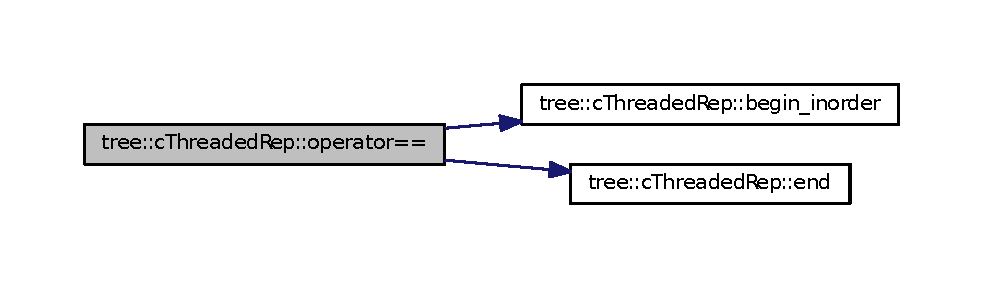
\includegraphics[width=350pt]{classtree_1_1cThreadedRep_a462ebaa3cc1325d075bf8ac280f65a9b_cgraph}
\end{center}
\end{figure}


\hypertarget{classtree_1_1cThreadedRep_a93489947fed29ed25fbb7268cbae049d}{\index{tree\-::c\-Threaded\-Rep@{tree\-::c\-Threaded\-Rep}!traverse@{traverse}}
\index{traverse@{traverse}!tree::cThreadedRep@{tree\-::c\-Threaded\-Rep}}
\subsubsection[{traverse}]{\setlength{\rightskip}{0pt plus 5cm}template$<$typename T $>$ template$<$typename F\-U\-N\-C $>$ void {\bf tree\-::c\-Threaded\-Rep}$<$ \-T $>$\-::{\bf traverse} (
\begin{DoxyParamCaption}
\item[{\-F\-U\-N\-C \&}]{visit}
\end{DoxyParamCaption}
)\hspace{0.3cm}{\ttfamily  \mbox{[}inline\mbox{]}}}}\label{classtree_1_1cThreadedRep_a93489947fed29ed25fbb7268cbae049d}
traverse the binary tree in the given tree\-\_\-traversal order takes a function object as a parameter, which must implement operator(\-T) 

\-The documentation for this class was generated from the following file\-:\begin{DoxyCompactItemize}
\item 
tree/threaded\-\_\-rep.\-h\end{DoxyCompactItemize}

\hypertarget{structFactorial}{\section{\-Factorial$<$ \-V\-A\-L $>$ \-Struct \-Template \-Reference}
\label{structFactorial}\index{\-Factorial$<$ V\-A\-L $>$@{\-Factorial$<$ V\-A\-L $>$}}
}
\subsection*{\-Public \-Types}
\begin{DoxyCompactItemize}
\item 
enum \{ {\bfseries value} =  \-V\-A\-L $\ast$ \-Factorial$<$\-V\-A\-L -\/ 1$>$\-:\-:value
 \}
\end{DoxyCompactItemize}
\subsubsection*{template$<$std\-::size\-\_\-t \-V\-A\-L$>$ struct Factorial$<$ V\-A\-L $>$}



\-The documentation for this struct was generated from the following file\-:\begin{DoxyCompactItemize}
\item 
factorial.\-h\end{DoxyCompactItemize}

\hypertarget{structFactorial_3_010_01_4}{
\section{\-Factorial$<$ 0 $>$ \-Struct \-Template \-Reference}
\label{structFactorial_3_010_01_4}\index{\-Factorial$<$ 0 $>$@{\-Factorial$<$ 0 $>$}}
}
\subsection*{\-Public \-Types}
\begin{DoxyCompactItemize}
\item 
enum \{ {\bfseries value} =  1
 \}
\end{DoxyCompactItemize}
\subsubsection*{template$<$$>$ struct Factorial$<$ 0 $>$}



\-The documentation for this struct was generated from the following file\-:\begin{DoxyCompactItemize}
\item 
factorial.\-h\end{DoxyCompactItemize}

\hypertarget{classMultiplication}{\section{Multiplication Class Reference}
\label{classMultiplication}\index{Multiplication@{Multiplication}}
}


{\ttfamily \#include $<$binary\-\_\-op.\-h$>$}



Collaboration diagram for Multiplication\-:
\subsection*{Public Member Functions}
\begin{DoxyCompactItemize}
\item 
\hypertarget{classMultiplication_abc832d7341a7f4a33054e41b8a6883da}{{\footnotesize template$<$typename T $>$ }\\T {\bfseries operator()} (const T \&ob1, const T \&ob2) const }\label{classMultiplication_abc832d7341a7f4a33054e41b8a6883da}

\end{DoxyCompactItemize}
\subsection*{Static Public Attributes}
\begin{DoxyCompactItemize}
\item 
\hypertarget{classMultiplication_a37f52c627c1caa3a1ba0388de58c5dbd}{static const bool {\bfseries is\-Additive} = false}\label{classMultiplication_a37f52c627c1caa3a1ba0388de58c5dbd}

\item 
\hypertarget{classMultiplication_aaf72f7c6c05f7ed984c8e997e0505d60}{static const bool {\bfseries is\-Multiplicative} = true}\label{classMultiplication_aaf72f7c6c05f7ed984c8e997e0505d60}

\item 
\hypertarget{classMultiplication_adbcbdd5feb18d22c1765fbe1b7829840}{static const bool {\bfseries is\-Composition} = false}\label{classMultiplication_adbcbdd5feb18d22c1765fbe1b7829840}

\end{DoxyCompactItemize}


\subsection{Detailed Description}
class that represents the multiplication binary operation used also as a template policy 

The documentation for this class was generated from the following file\-:\begin{DoxyCompactItemize}
\item 
binary\-\_\-op.\-h\end{DoxyCompactItemize}

\printindex
\end{document}
